\documentclass[12pt]{article}

\author{Matthew D. Cocci}
\title{Asset Pricing}
\date{\today}

%% Formatting & Spacing %%%%%%%%%%%%%%%%%%%%%%%%%%%%%%%%%%%%

%\usepackage[top=1in, bottom=1in, left=1in, right=1in]{geometry} % most detailed page formatting control
\usepackage{fullpage} % Simpler than using the geometry package; std effect
\usepackage{setspace}
%\onehalfspacing
\usepackage{microtype}

%% Formatting %%%%%%%%%%%%%%%%%%%%%%%%%%%%%%%%%%%%%%%%%%%%%

%\usepackage[margin=1in]{geometry}
    %   Adjust the margins with geometry package
%\usepackage{pdflscape}
    %   Allows landscape pages
%\usepackage{layout}
    %   Allows plotting of picture of formatting
\usepackage{multicol}
\setlength{\columnsep}{1cm}



%% Header %%%%%%%%%%%%%%%%%%%%%%%%%%%%%%%%%%%%%%%%%%%%%%%%%

%\usepackage{fancyhdr}
%\pagestyle{fancy}
%\lhead{}
%\rhead{}
%\chead{}
%\setlength{\headheight}{15.2pt}
    %   Make the header bigger to avoid overlap

%\fancyhf{}
    %   Erase header settings

%\renewcommand{\headrulewidth}{0.3pt}
    %   Width of the line

%\setlength{\headsep}{0.2in}
    %   Distance from line to text


%% Mathematics Related %%%%%%%%%%%%%%%%%%%%%%%%%%%%%%%%%%%

\usepackage{amsmath}
\usepackage{amssymb}
\usepackage{amsfonts}
\usepackage{mathrsfs}
\usepackage{amsthm} %allows for labeling of theorems
\theoremstyle{plain}
\newtheorem{thm}{Theorem}[section]
\newtheorem{lem}[thm]{Lemma}
\newtheorem{prop}[thm]{Proposition}
\newtheorem{cor}[thm]{Corollary}
\newtheorem{ax}[thm]{Axiom}

\theoremstyle{definition}
\newtheorem{defn}[thm]{Definition}
\newtheorem{ex}[thm]{Example}
\newtheorem{assump}[thm]{Assumption}

\theoremstyle{remark}
\newtheorem*{rmk}{Remark}
\newtheorem*{note}{Note}

% Below supports left-right alignment in matrices so the negative
% signs don't look bad
\makeatletter
\renewcommand*\env@matrix[1][c]{\hskip -\arraycolsep
  \let\@ifnextchar\new@ifnextchar
  \array{*\c@MaxMatrixCols #1}}
\makeatother


%% Font Choices %%%%%%%%%%%%%%%%%%%%%%%%%%%%%%%%%%%%%%%%%

\usepackage[T1]{fontenc}
\usepackage{lmodern}
\usepackage[utf8]{inputenc}
%\usepackage{blindtext}
\usepackage{courier}


%% Figures %%%%%%%%%%%%%%%%%%%%%%%%%%%%%%%%%%%%%%%%%%%%%%

\usepackage{tikz}
%\usepackage{tikz-3dplot}
\usetikzlibrary{decorations.pathreplacing}
\usetikzlibrary{patterns}
\usepackage{graphicx}
\usepackage{subfigure}
    %   For plotting multiple figures at once
%\graphicspath{ {Directory/} }
    %   Set a directory for where to look for figures

%\pgfdeclarepatternformonly[\LineSpace]{my north east lines}{\pgfqpoint{-1pt}{-1pt}}{\pgfqpoint{\LineSpace}{\LineSpace}}{\pgfqpoint{\LineSpace}{\LineSpace}}%
%{
    %\pgfsetlinewidth{0.4pt}
    %\pgfpathmoveto{\pgfqpoint{0pt}{0pt}}
    %\pgfpathlineto{\pgfqpoint{\LineSpace + 0.1pt}{\LineSpace + 0.1pt}}
    %\pgfusepath{stroke}
%}

%\pgfdeclarepatternformonly[\LineSpace]{my north west lines}{\pgfqpoint{-1pt}{-1pt}}{\pgfqpoint{\LineSpace}{\LineSpace}}{\pgfqpoint{\LineSpace}{\LineSpace}}%
%{
    %\pgfsetlinewidth{0.4pt}
    %\pgfpathmoveto{\pgfqpoint{0pt}{\LineSpace}}
    %\pgfpathlineto{\pgfqpoint{\LineSpace + 0.1pt}{-0.1pt}}
    %\pgfusepath{stroke}
%}

%\newdimen\LineSpace
%\tikzset{
    %line space/.code={\LineSpace=#1},
    %line space=3pt
%}


%% Hyperlinks %%%%%%%%%%%%%%%%%%%%%%%%%%%%%%%%%%%%%%%%%%%%
\usepackage{hyperref}
\hypersetup{%
    colorlinks,
        %   This colors the links themselves, not boxes
    citecolor=black,
        %   Everything here and below changes link colors
    filecolor=black,
    linkcolor=black,
    urlcolor=black
}

%% Colors %%%%%%%%%%%%%%%%%%%%%%%%%%%%%%%%%%%%%%%%%%%%%%%

\usepackage{color}
\definecolor{codegreen}{RGB}{28,172,0}
\definecolor{codelilas}{RGB}{170,55,241}

% David4 color scheme
\definecolor{d4blue}{RGB}{100,191,255}
\definecolor{d4gray}{RGB}{175,175,175}
\definecolor{d4black}{RGB}{85,85,85}
\definecolor{d4orange}{RGB}{255,150,100}


%% Including Code %%%%%%%%%%%%%%%%%%%%%%%%%%%%%%%%%%%%%%%

\usepackage{verbatim}
    %   For including verbatim code from files, no colors
\usepackage{listings}
    %   For including code snippets written directly in this doc

\lstdefinestyle{bash}{%
  language=bash,%
  basicstyle=\footnotesize\ttfamily,%
  showstringspaces=false,%
  commentstyle=\color{gray},%
  keywordstyle=\color{blue},%
  xleftmargin=0.25in,%
  xrightmargin=0.25in
}

\lstdefinestyle{matlab}{%
  language=Matlab,%
  basicstyle=\footnotesize\ttfamily,%
  breaklines=true,%
  morekeywords={matlab2tikz},%
  keywordstyle=\color{blue},%
  morekeywords=[2]{1}, keywordstyle=[2]{\color{black}},%
  identifierstyle=\color{black},%
  stringstyle=\color{codelilas},%
  commentstyle=\color{codegreen},%
  showstringspaces=false,%
    %   Without this there will be a symbol in
    %   the places where there is a space
  numbers=left,%
  numberstyle={\tiny \color{black}},%
    %   Size of the numbers
  numbersep=9pt,%
    %   Defines how far the numbers are from the text
  emph=[1]{for,end,break,switch,case},emphstyle=[1]\color{red},%
    %   Some words to emphasise
}

\newcommand{\matlabcode}[1]{%
    \lstset{style=matlab}%
    \lstinputlisting{#1}
}
    %   For including Matlab code from .m file with colors,
    %   line numbering, etc.

%% Bibliographies %%%%%%%%%%%%%%%%%%%%%%%%%%%%%%%%%%%%

\usepackage{natbib}
    %---For bibliographies
%\setlength{\bibsep}{3pt} % Set how far apart bibentries are


%% Misc %%%%%%%%%%%%%%%%%%%%%%%%%%%%%%%%%%%%%%%%%%%%%%

\usepackage{enumitem}
    %   Has to do with enumeration
\usepackage{appendix}
%\usepackage{natbib}
    %   For bibliographies
\usepackage{pdfpages}
    %   For including whole pdf pages as a page in doc


%% User Defined %%%%%%%%%%%%%%%%%%%%%%%%%%%%%%%%%%%%%%%%%%

%\newcommand{\nameofcmd}{Text to display}
\newcommand*{\Chi}{\mbox{\large$\chi$}} %big chi
    %   Bigger Chi

% In math mode, Use this instead of \munderbar, since that changes the
% font from math to regular
\makeatletter
\def\munderbar#1{\underline{\sbox\tw@{$#1$}\dp\tw@\z@\box\tw@}}
\makeatother

% Misc Math
\newcommand{\ra}{\rightarrow}
\newcommand{\diag}{\text{diag}}
\newcommand{\proj}{\operatorname{proj}}
\newcommand{\ch}{\text{ch}}
\newcommand{\dom}{\text{dom}}
\newcommand{\one}[1]{\mathbf{1}_{#1}}


% Command to generate new math commands:
% - Suppose you want to refer to \boldsymbol{x} as just \bsx, where 'x'
%   is any letter. This commands lets you generate \bsa, \bsb, etc.
%   without copy pasting \newcommand{\bsa}{\boldsymbol{a}} for each
%   letter individually. Instead, just include
%
%     \generate{bs}{\boldsymbol}{a,...,z}
%
% - Uses pgffor package to loop
% - Example with optional argument. Will generate \bshatx to represent
%   \boldsymbol{\hat{x}} for all letters x
%
%     \generate[\hat]{bshat}{\boldsymbol}{a,...,z}

\newcommand{\generate}[4][]{%
  % Takes 3 arguments (maybe four):
  % - 1   wrapcmd (optional, defaults to nothing)
  % - 2   newname
  % - 3   mathmacro
  % - 4   Names to loop over
  %
  % Will produce
  %
  %   \newcommand{\newnameX}{mathmacro{wrapcmd{X}}}
  %
  % for each X in argument 4

  \foreach \x in {#4}{%
    \expandafter\xdef\csname%
      #2\x%
    \endcsname%
    {\noexpand\ensuremath{\noexpand#3{\noexpand#1{\x}}}}
  }
}

% MATHSCR: Gen \sX to stand for \mathscr{X} for all upper case letters
\generate{s}{\mathscr}{A,...,Z}


% BOLDSYMBOL: Generate \bsX to stand for \boldsymbol{X}, all upper and
% lower case.
%
% Letters and greek letters
\generate{bs}{\boldsymbol}{a,...,z}
\generate{bs}{\boldsymbol}{A,...,Z}
\newcommand{\bseta}{\boldsymbol{\eta}}
\newcommand{\bstheta}{\boldsymbol{\theta}}
\newcommand{\bsTheta}{\boldsymbol{\Theta}}
\newcommand{\bsmu}{\boldsymbol{\mu}}
\newcommand{\bsSigma}{\boldsymbol{\Sigma}}
\newcommand{\bssigma}{\boldsymbol{\sigma}}
\newcommand{\bsvarepsilon}{\boldsymbol{\varepsilon}}
\newcommand{\bsalpha}{\boldsymbol{\alpha}}
\newcommand{\bsbeta}{\boldsymbol{\beta}}
\newcommand{\bsPi}{\boldsymbol{\Pi}}
\newcommand{\bsgamma}{\boldsymbol{\gamma}}
\newcommand{\bsGamma}{\boldsymbol{\Gamma}}
\newcommand{\bslambda}{\boldsymbol{\lambda}}
\newcommand{\bsLambda}{\boldsymbol{\Lambda}}
\newcommand{\bshatLambda}{\boldsymbol{\hat{\Lambda}}}
\newcommand{\bshatG}{\boldsymbol{\hat{G}}}
\newcommand{\bsdelta}{\boldsymbol{\delta}}
\newcommand{\bsOmega}{\boldsymbol{\Omega}}
\newcommand{\bsPsi}{\boldsymbol{\Psi}}
\newcommand{\bspsi}{\boldsymbol{\psi}}
\newcommand{\bsPhi}{\boldsymbol{\Phi}}
\newcommand{\bsphi}{\boldsymbol{\phi}}

% Special cases like \bshatb for \boldsymbol{\hat{b}}
\generate[\hat]{bshat}{\boldsymbol}{a,b,y,x,X,V,S,W,A,B,P}
\newcommand{\bshatbeta}{\boldsymbol{\hat{\beta}}}
\newcommand{\bshatmu}{\boldsymbol{\hat{\mu}}}
\newcommand{\bshattheta}{\boldsymbol{\hat{\theta}}}
\newcommand{\bsbartheta}{\boldsymbol{\bar{\theta}}}
\newcommand{\bshatSigma}{\boldsymbol{\hat{\Sigma}}}
\newcommand{\bstildebeta}{\boldsymbol{\tilde{\beta}}}
\newcommand{\bstildetheta}{\boldsymbol{\tilde{\theta}}}
\newcommand{\bstildePsi}{\boldsymbol{\tilde{\Psi}}}
\newcommand{\bsbarbeta}{\boldsymbol{\overline{\beta}}}
\newcommand{\bshatOmega}{\boldsymbol{\hat{\Omega}}}
\newcommand{\bsbarg}{\boldsymbol{\overline{g}}}
\newcommand{\bstildey}{\boldsymbol{\tilde{y}}}
\newcommand{\bstildeX}{\boldsymbol{\tilde{X}}}
\newcommand{\bstildevarepsilon}{\boldsymbol{\tilde{\varepsilon}}}
\newcommand{\bstildes}{\boldsymbol{\tilde{s}}}
\newcommand{\bstildeT}{\boldsymbol{\tilde{T}}}
\newcommand{\bstildeC}{\boldsymbol{\tilde{C}}}

% Zero vector as \bso
\renewcommand{\bso}{\boldsymbol{0}}

% Transposes of all the boldsymbol shit
\newcommand{\bsbp}{\boldsymbol{b'}}
\newcommand{\bshatbp}{\boldsymbol{\hat{b'}}}
\newcommand{\bsdp}{\boldsymbol{d'}}
\newcommand{\bsgp}{\boldsymbol{g'}}
\newcommand{\bsGp}{\boldsymbol{G'}}
\newcommand{\bshp}{\boldsymbol{h'}}
\newcommand{\bsSp}{\boldsymbol{S'}}
\newcommand{\bsup}{\boldsymbol{u'}}
\newcommand{\bsxp}{\boldsymbol{x'}}
\newcommand{\bsyp}{\boldsymbol{y'}}
\newcommand{\bsthetap}{\boldsymbol{\theta'}}
\newcommand{\bsmup}{\boldsymbol{\mu'}}
\newcommand{\bsSigmap}{\boldsymbol{\Sigma'}}
\newcommand{\bshatmup}{\boldsymbol{\hat{\mu'}}}
\newcommand{\bshatSigmap}{\boldsymbol{\hat{\Sigma'}}}

% MATHCAL: Gen \calX to stand for \mathcal{X}, all upper case
\generate{cal}{\mathcal}{A,...,Z}

% MATHBB: Gen \X to stand for \mathbb{X} for some upper case
\generate{}{\mathbb}{R,Q,C,Z,N,Z,E}
\newcommand{\Rn}{\mathbb{R}^n}
\newcommand{\RN}{\mathbb{R}^N}
\newcommand{\Rk}{\mathbb{R}^k}
\newcommand{\RK}{\mathbb{R}^K}
\newcommand{\RL}{\mathbb{R}^L}
\newcommand{\Rl}{\mathbb{R}^\ell}
\newcommand{\Rm}{\mathbb{R}^m}
\newcommand{\Rnn}{\mathbb{R}^{n\times n}}
\newcommand{\Rmn}{\mathbb{R}^{m\times n}}
\newcommand{\Rnm}{\mathbb{R}^{n\times m}}
\newcommand{\Rkn}{\mathbb{R}^{k\times n}}
\newcommand{\Cn}{\mathbb{C}^n}
\newcommand{\Cnn}{\mathbb{C}^{n\times n}}

% Dot over
\newcommand{\dx}{\dot{x}}
\newcommand{\ddx}{\ddot{x}}
\newcommand{\dy}{\dot{y}}
\newcommand{\ddy}{\ddot{y}}

% First derivatives
\newcommand{\dydx}{\frac{dy}{dx}}
\newcommand{\dfdx}{\frac{df}{dx}}
\newcommand{\dfdy}{\frac{df}{dy}}
\newcommand{\dfdz}{\frac{df}{dz}}

% Second derivatives
\newcommand{\ddyddx}{\frac{d^2y}{dx^2}}
\newcommand{\ddydxdy}{\frac{d^2y}{dx dy}}
\newcommand{\ddydydx}{\frac{d^2y}{dy dx}}
\newcommand{\ddfddx}{\frac{d^2f}{dx^2}}
\newcommand{\ddfddy}{\frac{d^2f}{dy^2}}
\newcommand{\ddfddz}{\frac{d^2f}{dz^2}}
\newcommand{\ddfdxdy}{\frac{d^2f}{dx dy}}
\newcommand{\ddfdydx}{\frac{d^2f}{dy dx}}


% First Partial Derivatives
\newcommand{\pypx}{\frac{\partial y}{\partial x}}
\newcommand{\pfpx}{\frac{\partial f}{\partial x}}
\newcommand{\pfpy}{\frac{\partial f}{\partial y}}
\newcommand{\pfpz}{\frac{\partial f}{\partial z}}

% argmin and argmax
\DeclareMathOperator*{\argmin}{arg\;min}
\DeclareMathOperator*{\argmax}{arg\;max}
\newenvironment{rcases}
  {\left.\begin{aligned}}
  {\end{aligned}\right\rbrace}

% Various probability and statistics commands
\newcommand{\wn}{\sim\operatorname{WN}}
\newcommand{\iid}{\overset{iid}{\sim}}
\newcommand{\vc}{\operatorname{vec}}
\newcommand{\Cov}{\operatorname{Cov}}
\newcommand{\range}{\operatorname{range}}
\newcommand{\Prb}{\operatorname{P}}
\newcommand{\rank}{\operatorname{rank}}
\newcommand{\trace}{\operatorname{trace}}
\newcommand{\Corr}{\operatorname{Corr}}
\newcommand{\Var}{\operatorname{Var}}
\newcommand{\asto}{\xrightarrow{a.s.}}
\newcommand{\pto}{\xrightarrow{p}}
\newcommand{\msto}{\xrightarrow{m.s.}}
\newcommand{\dto}{\xrightarrow{d}}
\newcommand{\Lpto}{\xrightarrow{L_p}}
\newcommand{\Lqto}[1]{\xrightarrow{L_{#1}}}
\newcommand{\plim}{\text{plim}_{n\rightarrow\infty}}

% Redefine real and imaginary from fraktur to plain text
\renewcommand{\Re}{\operatorname{Re}}
\renewcommand{\Im}{\operatorname{Im}}

% Shorter sums: ``Sum from X to Y''
% - sumXY  is equivalent to \sum^Y_{X=1}
% - sumXYz is equivalent to \sum^Y_{X=0}
\newcommand{\sumnN}{\sum^N_{n=1}}
\newcommand{\sumin}{\sum^n_{i=1}}
\newcommand{\sumjn}{\sum^n_{j=1}}
\newcommand{\sumim}{\sum^m_{i=1}}
\newcommand{\sumik}{\sum^k_{i=1}}
\newcommand{\sumiN}{\sum^N_{i=1}}
\newcommand{\sumkn}{\sum^n_{k=1}}
\newcommand{\sumtT}{\sum^T_{t=1}}
\newcommand{\sumninf}{\sum^\infty_{n=1}}
\newcommand{\sumtinf}{\sum^\infty_{t=1}}
\newcommand{\sumnNz}{\sum^N_{n=0}}
\newcommand{\suminz}{\sum^n_{i=0}}
\newcommand{\sumknz}{\sum^n_{k=0}}
\newcommand{\sumtTz}{\sum^T_{t=0}}
\newcommand{\sumninfz}{\sum^\infty_{n=0}}
\newcommand{\sumtinfz}{\sum^\infty_{t=0}}
\newcommand{\sumsinfz}{\sum^\infty_{s=0}}

\newcommand{\prodnN}{\prod^N_{n=1}}
\newcommand{\prodin}{\prod^n_{i=1}}
\newcommand{\prodiN}{\prod^N_{i=1}}
\newcommand{\prodkn}{\prod^n_{k=1}}
\newcommand{\prodtT}{\prod^T_{t=1}}
\newcommand{\prodnNz}{\prod^N_{n=0}}
\newcommand{\prodinz}{\prod^n_{i=0}}
\newcommand{\prodknz}{\prod^n_{k=0}}
\newcommand{\prodtTz}{\prod^T_{t=0}}

% Bounds
\newcommand{\atob}{_a^b}
\newcommand{\ztoinf}{_0^\infty}
\newcommand{\kinf}{_{k=1}^\infty}
\newcommand{\ninf}{_{n=1}^\infty}
\newcommand{\minf}{_{m=1}^\infty}
\newcommand{\tinf}{_{t=1}^\infty}
\newcommand{\nN}{_{n=1}^N}
\newcommand{\tT}{_{t=1}^T}
\newcommand{\kinfz}{_{k=0}^\infty}
\newcommand{\ninfz}{_{n=0}^\infty}
\newcommand{\minfz}{_{m=0}^\infty}
\newcommand{\tinfz}{_{t=0}^\infty}
\newcommand{\tTz}{_{t=0}^T}

% Limits
\newcommand{\limN}{\lim_{N\rightarrow\infty}}
\newcommand{\limn}{\lim_{n\rightarrow\infty}}
\newcommand{\limk}{\lim_{k\rightarrow\infty}}
\newcommand{\limt}{\lim_{t\rightarrow\infty}}
\newcommand{\limT}{\lim_{T\rightarrow\infty}}
\newcommand{\limhz}{\lim_{h\rightarrow 0}}

% Shorter integrals: ``Integral from X to Y''
% - intXY is equivalent to \int^Y_X
\newcommand{\intab}{\int_a^b}
\newcommand{\intzN}{\int_0^N}



%%%%%%%%%%%%%%%%%%%%%%%%%%%%%%%%%%%%%%%%%%%%%%%%%%%%%%%%%%%%%%%%%%%%%%%%
%% BODY %%%%%%%%%%%%%%%%%%%%%%%%%%%%%%%%%%%%%%%%%%%%%%%%%%%%%%%%%%%%%%%%
%%%%%%%%%%%%%%%%%%%%%%%%%%%%%%%%%%%%%%%%%%%%%%%%%%%%%%%%%%%%%%%%%%%%%%%%



\begin{document}
\maketitle

\tableofcontents


\clearpage
\begin{multicols*}{2}
\section{Key Formulas}

\subsection{Prices and Payoffs}

Agent problem: two periods, endowments $e_t$ and $e_{t+1}$, rate
of \emph{time} (but \emph{not} risk) discounting $\beta$. Can buy/sell
any amount of asset,\footnote{
  Critical assumption.
  Implies agent can make \emph{arbitrarily small} portfolio adjustments,
  hence justified in using FOCs to characterize optimum.
  Thus price $p_t$ will be a \emph{marginal} concept---what an investor
  would pay to hold a tiny extra piece of the asset.
  Doesn't work for large venture cap all-or-nothing type investments.
}
price $p_t$, payoff $x_{t+1}$ (RV realized $t+1$).
\begin{align*}
  \max_{\xi\in\R}
  \;
  &u(c_t) + \beta\E_t[u(c_{t+1})] \\
  \text{s.t.}\qquad
  c_t &= e_t - \xi p_t \\
  c_{t+1} &= e_{t+1} + \xi x_{t+1}
\end{align*}
FOCs give price in terms of \emph{stochastic discount factor}
$m_{t+1}$ (also a RV),\footnote{%
  $m_{t+1}$ also sometimes called marginal rate of substitution, state
  price density, change of measure
}
\begin{align}
  p_t = \E_t[m_{t+1}x_{t+1}],
  \quad
  m_t := \beta \frac{u'(c_{t+1})}{u'(c_t)}
  \label{pemx}
  %\\
  %\text{where}\quad
  %m_t :=&\; \beta \frac{u'(c_{t+1})}{u'(c_t)}
  %\label{mdf}
\end{align}
Eq.~\ref{pemx} holds \emph{after} agent has made all
desired investments \& reached optimal allocation.
\footnote{%
  For utility, we often use \emph{power utility}
  $u(c) = \frac{c^{1-\gamma}-1}{1-\gamma}$
  which implies $u(c)=\log(c)$ as $\gamma\ra 1$ and
  $u'(c) = c^{-\gamma}$
}

\emph{Returns} have unit price, RV payoff $R_{t+1}$:
\begin{align}
  1 &= \E_t[m_{t+1}R_{t+1}]
  \label{ret}
\end{align}
Eq.~\ref{pemx} is a map/operator $p[x]$ from RV payoff $x(\omega)$ to
price $p$. Eq.~\ref{ret} is instead a condition that a unit-price asset
(a return) must satisfy.
Payoffs across states $R(\omega)$ co-move with $m(\omega)$
such that Eq.~\ref{ret} holds.

\emph{Excess return} $R^e=R^i-R^j$ is long return $R^i$, short $R^j$.
With both $R^i,R^j$ unit price, portfolio is zero cost:
\begin{align*}
  0 = \E_t[m_{t+1}R^e_{t+1}]
  %= \E_t[m_{t+1}(R^i_{t+1}-R_{t+1}^j)]
\end{align*}
\emph{Risk-free rate} $R^f$ satisfies $\E_t[R^f_{t+1}]=R^f_{t+1}$
(though $R^f_t\neq R^f_s$), hence Eq.~\ref{ret} gives
\begin{align}
  R^f
  &= 1/\;\E[m]
  \label{rf}
\end{align}
To interpret pricing Eq.~\ref{pemx}, use Eq.~\ref{rf} and
$\Cov(x,y)=\E[xy] - \E[x]\E[y]$ on $\E[mx]$:
\begin{align}
  p =  \frac{\E[x]}{R^f} + \Cov(m,x)
  \label{riskadj}
\end{align}
Price is discounted expected payoff plus a risk
correction for covariance of payoff $x$ with $m$.
Risk neutrality implies $u'$, hence $m$, constant, in which case
$\Cov(m,x)=0$.

If $x_{t+1}$ is a return $R^i$, the above becomes
\begin{align}
  \E[R^i] - R^f =  -R^f \Cov(m,R^i)
  \label{riskadjret}
\end{align}
Thus assets only generate average excess (above $R^f$) returns if
correlated with $m$.

\subsection{Contingent Claims}

Let $pc(\omega)$ denote price of a \emph{contingent claim} paying \$1
if state $\omega$ realized, \$0 otherwise.
Assume \emph{complete markets} with a contingent claim traded
for each $\omega$, hence $pc(\omega)$ defined $\forall
\omega\in\Omega$.\footnote{
  Don't strictly need contingent claims $\forall\omega$.
  But must be able to synthesize/replicate with other traded assets.
  If fewer assets traded than total no. of states, can get
  complete markets if \emph{dynamic trading} allowed.
}
Can price any payoff $x:\Omega\ra\R$
\begin{align}
  p[x]
  = \sum_\omega pc(\omega) x(\omega)
  \label{eq:contingentprice}
\end{align}
Letting $\pi(\omega)$ denote state probs, can get discount factor $m$
and pricing Eq.~\ref{pemx}
\begin{align*}
  p[x]
  &= \sum_\omega
  \pi(\omega)
  \underbrace{%
  \left(
  \frac{pc(\omega)}{\pi(\omega)}
  \right)
  }_{m(\omega)}
  x(\omega)
  = \E[mx]
\end{align*}
Alternatively, can also rewrite Equation~\ref{eq:contingentprice} using
\emph{risk neutral probs} $\pi^*(\omega)$
\begin{align*}
  p[x]
  &= \frac{1}{R^f} \sum_\omega
  \underbrace{R^f pc(\omega)}_{\pi^*(\omega)}x(\omega)
  = \frac{\E^*[x(\omega)]}{R^f}
\end{align*}


\clearpage
\subsection{Continuous Time}

Agent maximizes utility given endowment by buying/selling asset over
time, which pays dividends continuously at rate $D_t$ per unit time and
has price $p_t$ following a diffusion:\footnote{%
  Price follows
  $dp_t/p_t = \mu(\,\cdot\,)\; dt + \sigma(\,\cdot\,) \; dW_t$
  where $\mu(\,\cdot\,)$ and $\sigma(\,\cdot\,)$ are functions that can
  depend upon $t$, $p_t$, or other state variables, allowing
  us to generate non-Gaussian dynamics (though $W_t$ normal).
}
\begin{align*}
  \max \;
  \E_t \int_{0}^\infty e^{-\rho s} u(c_{t+s})\; ds
\end{align*}
FOCs involving $\Lambda_t$, analogue of SDF $m_{t+1}$ that represents
discounted level of MU:
%\begin{align*}
  %p_tu'(c_t)
  %= \E_t
  %\int_{0}^\infty e^{-\delta s} u'(c_{t+s})D_{t+s}\; ds
%\end{align*}
%Equivalently, we have
\begin{align}
  p_t\Lambda_t
  =&\; \E_t
  \int_{0}^\infty \Lambda_{t+s}D_{t+s}\; ds
  \label{pemxcont1}
  \\
  \Lambda_t :=&\; e^{-\rho t} u'(c_t)
\end{align}
Difference Eq.~\ref{pemxcont1} between $t+\Delta$ and $t$, take cond.
exp. $\E_t$ of both sides, send $\Delta\ra 0$, rearrange to get
fundamental pricing eq.
%\begin{align*}
  %\E_t
  %\left[
  %\Lambda_{t+\Delta}p_{t+\Delta}
  %-\Lambda_tp_t
  %\right]
  %\\
  %&= \E_t\left[
  %\int_{0}^\infty \Lambda_{t+\Delta+s}D_{t+\Delta+s}\; ds
  %-
  %\int_{0}^\infty \Lambda_{t+s}D_{t+s}\; ds
  %\right]
  %\\
  %&=
  %-\E_t
  %\int_{0}^\Delta \Lambda_{t+s}D_{t+s}\; ds
  %\\
  %\implies\quad
%\end{align*}
%Sending $\Delta\ra 0$ and rearranging, we get
%fundamental pricing equation
\begin{align}
  \boxed{%
  0 = \Lambda_t D_t \;dt + \E_t[d(\Lambda_tp_t)]
  }
  \label{pemxcont2}
\end{align}
If $D_t=0$, martingale MU-weighted price.

Use Ito's Lemma to break up $d(\Lambda_tp_t)$, obtain equivalent
fundamental pricing eqn:
\begin{align*}
  \boxed{%
  0 = \Lambda D \,dt
  + \E_t[p \,d\Lambda + \Lambda \, dp + d\Lambda \,dp]
  }
  %\label{pemxcont3}
\end{align*}
If $\Lambda$ and $p$ never zero, divide through by $\Lambda p$:
\begin{align}
  \boxed{%
  0 = \frac{D}{p} \,dt
  + \E_t\left[
    \frac{d\Lambda}{\Lambda} + \frac{dp}{p}
    + \frac{d\Lambda}{\Lambda}\frac{dp}{p}
    \right]
  }
  \label{pemxcont4}
\end{align}
Now \emph{returns}.
Holding the asset at $t$ earns total \emph{net payoff} $dp_t + D_t dt$
over the next instant. Hence total instantaneous \emph{net return} at
$t$
%(denoted $dR_t$\footnote{
  %To see that $dR_t$ is the proper notation for a net return, consider a
  %net return in discrete time, which equals
  %$R_{t+1}-1= (p_{t+1}+D_{t+1})/p_t - p_t/p_t=R_{t+1}-R_t$.
%})
is given by that net payoff over price
\begin{align}
  %dR_t =
  \frac{dp_t}{p_t}
  + \frac{D_t}{p_t} dt
  \label{returnscont}
\end{align}
The \emph{risk free asset} pays instantaneous net return
%$dR_t=r^f_t dt$,
$r^f_t dt$.\footnote{%
  $r^f_t$ is the level of the risk free rate at $t$.
  As in discrete time, even though $r^f_t\neq r^f_s$ in general, it is
  ``risk free'' in sense that the net rate of return over the next
  instant has no Brownian term and is simply $r^f_t\;dt$.
}
Equating with Eq.~\ref{returnscont}, we see two ways to model this
asset: (i) Constant $p_t=1$ with $D_t=r_t^f$
or (ii) $dp_t/p_t=r^f_t\;dt$ with $D_t=0$.
Using either in Eq.~\ref{pemxcont4}, we can get the continuous time
analog of Eq.~\ref{rf}:
\begin{align}
  r^f_t\;dt =
  -\E_t\left[ \frac{d\Lambda_t}{\Lambda_t} \right]
  \label{rfcts}
\end{align}
Now use Eq.~\ref{rfcts} to get the continuous time analog of the risk
adjustment formula (\ref{riskadjret})
\begin{align*}
  \E_t\left[
     \frac{dp_t}{p_t}
  \right]
  +
  \frac{D_t}{p_t} dt
  =
  r^f_t\;dt
  - \E_t\left[
     \frac{d\Lambda_t}{\Lambda_t}\frac{dp_t}{p_t}
    \right]
  %\label{pemxcont5}
\end{align*}


\clearpage
\subsection{State Space Geometry}

For this section, assume finite state space
$\Omega=\{\omega_1,\ldots,\omega_S\}$.\footnote{%
  Everything generalizes to the infinite case with careful math.
}
Therefore, any state-contingent payoff $x(\omega)$ can be represented as
a vector in $\R^S$
\begin{align*}
  \bsx
  &:= \big(x(\omega_1),\; \ldots,\; x(\omega_S)\big)'
  \in\R^S
\end{align*}
Define \emph{payoff space} $\underline{X}\subseteq \R^S$ as the set of
all payoffs that can be bought, sold, or synthesized
$a\bsx_1 + b\bsx_2$ for $a,b\in\R$ and $\bsx_1,\bsx_2\in\underline{X}$.
(Assumes free portfolio formation, i.e. no bid-ask
spread, short-sale constraints, etc.)

A market is \emph{complete} if $\underline{X}=\R^S$, \emph{incomplete}
if $\underline{X}\subsetneq\R^S$. In a complete market, contingent
claims to all states of nature either exist or can be
replicated/synthesized.

\subsubsection{Complete Markets}

Contingent claim price vector $\underline{X}=\R^S$:
\begin{align*}
  \bsp\bsc
  &:= \big(pc(\omega_1),\; \ldots,\; pc(\omega_S)\big)'
  \in\R^S
\end{align*}
Hence pricing Eq.~\ref{eq:contingentprice} is just an inner product
\begin{align}
  p[x]=\langle \bsp\bsc, \bsx\rangle
  = \lVert \bsp\bsc\rVert \times \lVert \proj(\bsx|\bsp\bsc)\rVert
  \label{vectorprice}
\end{align}
Second equality is a property of inner products. It implies
\emph{identical price hyperplanes} in $\R^{S-1}$, which lie at right
angles to $\bsp\bsc\in\R^S$ \& connect payoffs $\bsx\in\R^S$ of
identical price.
If $S=2$, the payoff space looks like
\vspace{10pt}

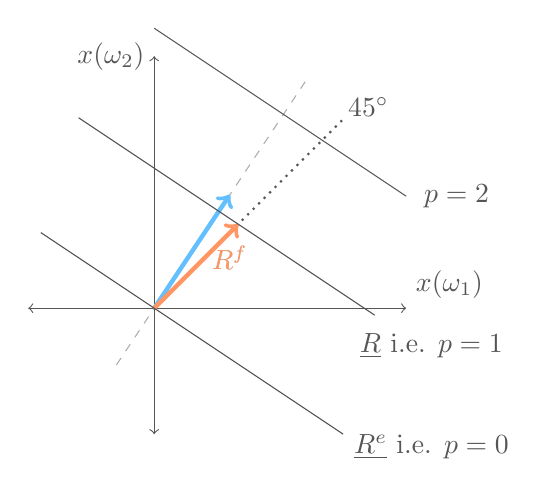
\begin{tikzpicture}[xscale=1.6, yscale=1.6] %, shorten >= 3pt
  % Axes
  \draw[d4black, <->] (0,-1) -- (0,0) -- (0,2)
                      node[left]{$x(\omega_2)$};
  \draw[d4black, <->] (-1,0) -- (0,0) -- (2,0)
                      node[above right]{$x(\omega_1)$};

  % Contingent claims price vector, pc = (0.6, 0.9)
  % Hence p = 0.6x1 + 0.9x2 => x2 = (10/9)p - (2/3) x1
  \draw[d4gray, dashed] (-0.3,-0.45) -- (1.2,1.8);
  \draw[d4blue, ultra thick, ->] (0.0,0.0) -- (0.6,0.9);
  \node[d4gray] at (0.5,1.05) {$\bsp\bsc$};
  \node[d4blue] at (0.5,1.05) {$\bsp\bsc$};

  % Risk free rate
  \draw[d4black, thick, dotted] (0.0,0.0) -- (1.5,1.5);
  \node[d4black] at (1.7,1.6) {$45^{\circ}$};
  \draw[d4orange, ultra thick, ->] (0.0,0.0) -- (0.6666666,0.6666666);
  \node[d4gray] at (0.6,0.4) {$R^f$};
  \node[d4orange] at (0.6,0.4) {$R^f$};

  % Space of excess returns, x2 = -(2/3) x1
  \draw[d4black, thin] (-0.9, 0.6) -- (1.5, -1.0);
  \node[d4black] at (2.2,-1.1) {$\underline{R^e}$ i.e. $p=0$};

  % Space of returns, x2 = (10/9) - (2/3) x1
  \draw[d4black, thin] (-0.6, 1.5111111) -- (1.75,-0.05555555);
  \node[d4black] at (2.2,-0.3) {$\underline{R}$ i.e. $p=1$};

  % Space of p=2, x2 = (10/9)*2 - (2/3) x1
  \draw[d4black, thin] (0.0, 2.2222222) -- (2,0.88888888);
  \node[d4black] at (2.4,0.888888888) {$p=2$};
\end{tikzpicture}
%\begin{align*}
  %pc &= (0.6, \; 0.9)\\
 %p &= 0.6x_1 +  0.9x_2 \\
  %x_2 &= \frac{10}{9}p - \frac{2}{3}x_1
%\end{align*}

We can also use vector geometry to understand $p=\E[mx]$, i.e.\ pricing
with SDF
\begin{align*}
  \bsm=(m(\omega_1),\ldots,m(\omega_S))\in\R^S
\end{align*}
instead of contingent claims prices $pc(\omega)$.
To do so, simply switch the underlying inner product and norm from
Euclidean to $L^2$:
\begin{align*}
  \langle x,y \rangle := \E[xy]
  \qquad
  \lVert x\rVert := \sqrt{\E[x^2]}
\end{align*}
%What's more, we even have a version of Expression~\ref{vectorprice}:
%\begin{align*}
  %\langle x,y \rangle
  %= \lVert y\rVert \times \lVert \proj(x|y)\rVert
%\end{align*}
\emph{However}, important note:
we will continue to draw vectors, visualize projections, and reason in
Euclidean space. We use this visual metapher \emph{even though} every
dot/inner product is really $\E[xy]$ underneath, involving RVs $x,y$
rather than vectors $\bsx,\bsy$.

For example, we update the picture to
\vspace{10pt}

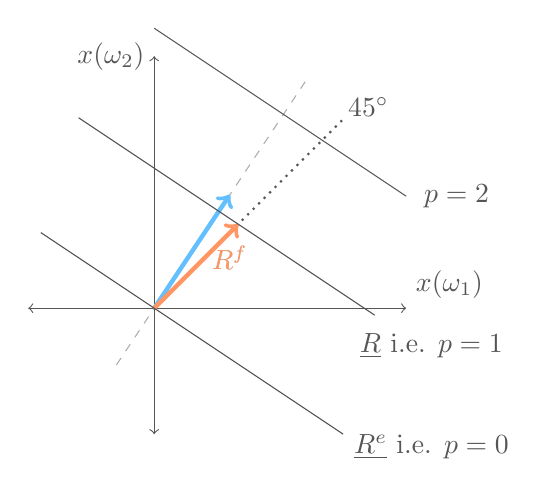
\begin{tikzpicture}[xscale=1.6, yscale=1.6] %, shorten >= 3pt
  % Axes
  \draw[d4black, <->] (0,-1) -- (0,0) -- (0,2)
                      node[left]{$x(\omega_2)$};
  \draw[d4black, <->] (-1,0) -- (0,0) -- (2,0)
                      node[above right]{$x(\omega_1)$};

  % Contingent claims price vector, pc = (0.6, 0.9)
  % Hence p = 0.6x1 + 0.9x2 => x2 = (10/9)p - (2/3) x1
  \draw[d4gray, dashed] (-0.3,-0.45) -- (1.2,1.8);
  \draw[d4blue, ultra thick, ->] (0.0,0.0) -- (0.6,0.9);
  \node[d4gray] at (0.5,1.05) {$\bsp\bsc$};
  \node[d4blue] at (0.5,1.05) {$\bsp\bsc$};

  % Risk free rate
  \draw[d4black, thick, dotted] (0.0,0.0) -- (1.5,1.5);
  \node[d4black] at (1.7,1.6) {$45^{\circ}$};
  \draw[d4orange, ultra thick, ->] (0.0,0.0) -- (0.6666666,0.6666666);
  \node[d4gray] at (0.6,0.4) {$R^f$};
  \node[d4orange] at (0.6,0.4) {$R^f$};

  % Space of excess returns, x2 = -(2/3) x1
  \draw[d4black, thin] (-0.9, 0.6) -- (1.5, -1.0);
  \node[d4black] at (2.2,-1.1) {$\underline{R^e}$ i.e. $p=0$};

  % Space of returns, x2 = (10/9) - (2/3) x1
  \draw[d4black, thin] (-0.6, 1.5111111) -- (1.75,-0.05555555);
  \node[d4black] at (2.2,-0.3) {$\underline{R}$ i.e. $p=1$};

  % Space of p=2, x2 = (10/9)*2 - (2/3) x1
  \draw[d4black, thin] (0.0, 2.2222222) -- (2,0.88888888);
  \node[d4black] at (2.4,0.888888888) {$p=2$};
\end{tikzpicture}

\clearpage
\subsubsection{Incomplete Markets}

Assume $\underline{X}\subsetneq \R^S$, i.e. tradeable assets don't
\emph{span} the state space. For ex, the figure below shows
$\dim(\underline{X})=2<S=3$. $\underline{X}$ is a plane extending out
from the triangle.

\vspace{10pt}
%\tdplotsetmaincoords{70}{15}
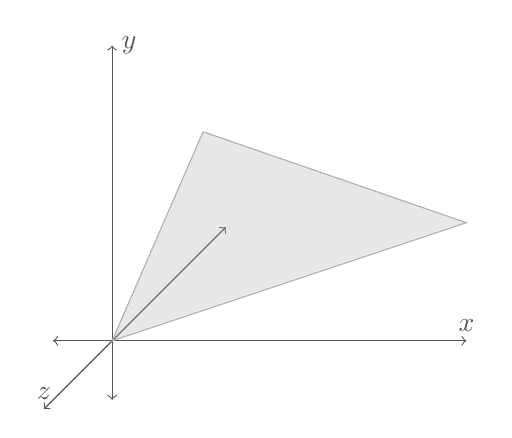
\begin{tikzpicture}[scale=1.5] %,tdplot_main_coords
    % Define axes
    \draw[d4black,<->] (-0.5,0,0) -- (3,0,0) node[above]{$x$};
    \draw[d4black,<->] (0,-0.5,0) -- (0,2.5,0) node[right]{$y$};
    \draw[d4black,<->] (0,0,-2.5) -- (0,0,1.5) node[anchor=south]{$z$};

    % Draw the plane
    \fill[
        draw=d4gray,%
        fill=d4gray,%
        fill opacity=0.3,%
    ] (0,1,-2)
      -- (3,1,0)
      -- (0,0,0)
      -- cycle;

    % Draw reference points
    %\node[d4black] at (0.7,0.7,1.8) {$b$};
\end{tikzpicture}
\\
\emph{Goal}: Suppose we don't have an economic model giving SDF $m$
pricing payoffs $x\in\underline{X}$ according to $p=\E[mx]$.
Can we go backwards and \emph{find} a SDF to price assets?

\begin{assump}
For all $x_1,x_2\in \underline{X}$ and $a,b\in\R$, we might assume
\begin{itemize}
  \item[A1.] \emph{Portfolio formation}:
    $ax_1+bx_2\in\underline{X}$.
  \item[A2.] \emph{Linearity/Law Of One Price} (LOOP):
    $p[ax_1+bx_2] = ap[x_1]+bp[x_2]$.
    \footnote{
      Note: people colloquially use ``no arb'' to refer to
      violations of A2/LOOP, \emph{not} A3 (which is stronger).
    }
  \item[A3.] \emph{No Arbitrage}:
    If $x(\omega)\geq x'(\omega)$ $\forall \omega\in\Omega$,
    strict for at least one $\omega$, $p[x]>p[x']$.

    With A1-2, equivalent to:
    If $x(\omega)\geq 0$ $\forall\omega$,
    strict for at least one, $p[x]>0$.
    (``No free assets that might pay'')
\end{itemize}
\end{assump}

\begin{thm}
We care about two directions
\begin{itemize}
  \item
    \emph{($\Rightarrow$)}
    Given SDF $m$ from an economic model pricing all assets/payoffs in
    $\R^S$ by $p=\E[mx]$, A2 (LOOP) holds.
  \item
    \emph{($\Leftarrow$)}
    Assuming A1 \& A2, $\exists\,!$ a discount factor
    $x^*\in\underline{X}$ pricing all assets in $\underline{X}$,
    i.e. s.t. $p=\E[x^*x]$ for all $x\in\underline{X}$
\end{itemize}
\end{thm}
\begin{proof}
($\Rightarrow$) $p[ax_1+bx_2] = \E[m(ax_1+bx_2)]$. Linearity of
$\E$ to conclude.

($\Leftarrow$) First, A1-2 imply \emph{parallel, linear} price
hyperplanes in $\underline{X}$.
Figure below depicts this for $\dim(\underline{X})=2$.
Dashed line $\perp$ to the price planes
pins down direction of $x^*$.
Then just fix length so $1=\E[x^*R]$ $\forall R\in\underline{R}$.

\vspace{10pt}

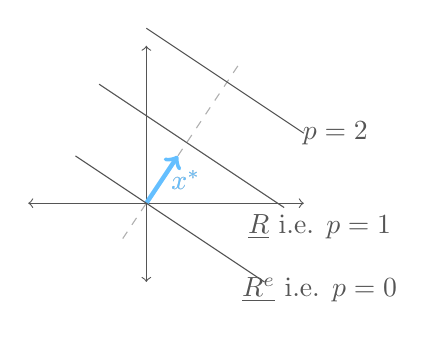
\begin{tikzpicture}[xscale=1, yscale=1] %, shorten >= 3pt
  % Axes
  \draw[d4black, <->] (0,-1) -- (0,0) -- (0,2);
  \draw[d4black, <->] (-1.5,0) -- (0,0) -- (2,0);

  % Contingent claims price vector, pc = (0.6, 0.9)
  % Hence p = 0.6x1 + 0.9x2 => x2 = (10/9)p - (2/3) x1
  \draw[d4gray, dashed] (-0.3,-0.45) -- (1.2,1.8);
  \draw[d4blue, ultra thick, ->] (0.0,0.0) -- (0.4,0.6);
  \node[d4gray] at (0.5,0.3) {$x^*$};
  \node[d4blue] at (0.5,0.3) {$x^*$};

  % Space of excess returns, x2 = -(2/3) x1
  \draw[d4black, thin] (-0.9, 0.6) -- (1.5, -1.0);
  \node[d4black] at (2.2,-1.1) {$\underline{R^e}$ i.e. $p=0$};

  % Space of returns, x2 = (10/9) - (2/3) x1
  \draw[d4black, thin] (-0.6, 1.5111111) -- (1.75,-0.05555555);
  \node[d4black] at (2.2,-0.3) {$\underline{R}$ i.e. $p=1$};

  % Space of p=2, x2 = (10/9)*2 - (2/3) x1
  \draw[d4black, thin] (0.0, 2.2222222) -- (2,0.88888888);
  \node[d4black] at (2.4,0.888888888) {$p=2$};
\end{tikzpicture}
\\
Algebra: If $\dim(\underline{X})=N\leq S$, can choose $N$ basis payoffs
in $\underline{X}$ that span. Stack these payoffs \& their prices
into vectors
$X(\omega):=(x_1(\omega)\ldots x_N(\omega))'$ and
$P:=(p_1\ldots p_N)'$

Since $x^*\in\underline{X}$ and assets in $X$ span $\underline{X}$, must
be $x^*=X'c$ for some weights $c$. Construct $c$ so $x^*$ prices basis
assets:
\begin{align*}
  P &= \E[x^*X] = \E[X(X'c)] = \E[XX']c
\end{align*}
We can solve for $c$ to get
\begin{align*}
  %\implies\;
  %c &= \E[XX']^{-1}P \\
  %\implies
  x^* &= P'\;\E[XX']^{-1}X
\end{align*}
Clearly, $x^*\in\underline{X}$, unique, prices assets in $X$ by
construction, and since they span $\underline{X}$, those assets can
replicate any other payoff in $\underline{X}$. So by A2, $x^*$ prices
everything else.
\end{proof}


\begin{cor}
Regarding unique $x^*\in \underline{X}$:
\begin{enumerate}[label=\emph{(\roman*)}]
  \item $\dim(\underline{X})=S$ implies $x^*$ unique in $\R^S$.
  \item $\underline{X}\subsetneq \R^S$ implies infinitely many
    SDFs that price all assets $x\in\underline{X}$ by
    formula $p=\E[\tilde{x}^*x]$ where
    \begin{align*}
      \tilde{x}^*
      = x^* + \varepsilon
      \;\;
      \text{where}\;
      \E[\varepsilon x] = 0,
      \; \forall x\in\underline{X}
    \end{align*}
  \item If $m$ is the unique, true SDF pricing all payoffs in $\R^S$,
    $x^*=\proj(m|\underline{X})$.
\end{enumerate}
\end{cor}

%Since $x^*\in\underline{X}$, it's clear that we might have
%$x^*(\omega)=0$ for some $\omega\in\Omega$.

\clearpage

Our next goal is to extend SDF $x^*\in\underline{X}$ (which prices
payoffs in $\underline{X}$) to ensure that we can \emph{also} price
payoffs in $\R^S\setminus\underline{X}$ \emph{without} implying
arbitrage opportunities.

While the last theorem guaranteed a unique $x^*\in\underline{X}$, it
did \emph{not} guarantee a \emph{strictly positive} $x^*$---and that's
\emph{key} for preventing arbitrage $\R^S\setminus\underline{X}$.
For example, suppose $\underline{X}\subsetneq\R^S$ is zero along
some axis. In other words, there exists a $\omega'\in\Omega$ such that
\begin{align*}
  x(\omega') = 0
  \qquad \forall x\in \underline{X}
\end{align*}
Then $x^*\in\underline{X}$ necessarily has $x^*(\omega')=0$.
But that could imply arbitrage opportunties (free portfolios that might
pay) if we try to price assets/payoffs \emph{outside} of
$\underline{X}$.

\begin{thm}
Again, two directions
\begin{itemize}
  \item \emph{($\Rightarrow$):}
    SDF $m$ from an economic model pricing all assets/payoffs
    in $\R^S$ by $p=\E[mx]$ plus A1 imply A2-3 hold.
  \item
    \emph{($\Leftarrow$):}
    Given A1-3, $\exists$ a
    \emph{strictly positive}\footnote{
      i.e. $m^*(\omega)>0$ for all $\omega\in\Omega$
    }
    SDF $m^*\in\R^S$ pricing all payoffs
    \begin{align*}
      p=\E[m^*x]
      \qquad
      \forall
      x\in \R^S\supseteq \underline{X}
    \end{align*}
    Note $m^*$ generally not unique or in $\underline{X}$ unless
    $\dim(\underline{X})=S$.
    Typically,
    \begin{align*}
      m^*=x^*+\varepsilon
      \;\text{where}\;
      \E[\varepsilon x]=0,\,
      \forall x\in\underline{X}
    \end{align*}
    All such SDFs agree about prices of
    $x\in\underline{X}$, generally disagree for
    $x\not\in\underline{X}$.
\end{itemize}
\end{thm}
\begin{proof}
($\Rightarrow$)
A2 holds by previous thm.
Since $m$ from economic model, it represents MU and is strictly
positive $m(\omega)>0$. Hence, for $x(\omega)\geq 0$ with $x(\omega')>0$
for at least one $\omega'$, clearly have $\E[mx]>0$, hence A3.
\\
\\
($\Leftarrow$)
A3/no-arb means any payoff in the nonnegative orthant of
$\R^S$ (excluding the origin) has positive price.
Again, there are parallel, linear price planes cutting through
$\underline{X}$.\footnote{%
  If $\dim(\underline{X})<S$, we have some freedom in the angle at which
  they cut through $\underline{X}$; otherwise, pinned down.
}
That includes the zero price plane, which intersects the nonnegative
orthant only at the origin. Thus $\exists$ a separating hyperplane
through the origin, separating the zero price hyperplane and
nonnegative orthant, with perpendicular vector pointing into the
positive orthant. This perpendicular vector pins down the direction of
$m^*$. To pin down length, simply normalize so it prices all returns
$1=\E[m^*R]$.
\end{proof}

\clearpage
\subsection{Representative Agent}

A representative agent is endowed with a marketable \emph{wealth portfolio}
that can be used to purchase consumption.
Into this wealth portfolio is capitalized \emph{everything} the agent
has that generates purchasing power: financial assets providing
dividends/returns, human capital generating labor income, etc.  This
wealth portfolio has current market value $W_t$ (in units of current
consumption $C_t$), i.e. one unit of the wealth portfolio can be traded
for one unit of consumption, and $W_t$ is max feasible
current consumption.

After consumption purchases, all remaining wealth $W_t-C_t$ is
reinvested to provide for future consumption, earning random
\emph{return on wealth} $R^W_{t+1}$ (which includes returns to financial
assets, returns to human capital aka labor income, etc.) that
generates additional purchasing power for the next period.
Hence, next period wealth $W_{t+1}$ satisfies intertemporal
budget constraint
\begin{align*}
  W_{t+1} = R_{t+1}^W(W_t-C_t)
\end{align*}
Defining $\tilde{W}_t:=W_t-C_t$, rearrange to get
\begin{align}
  R_{t+1}^W
  = \frac{W_{t+1}}{W_t-C_t}
  = \frac{\tilde{W}_{t+1}+C_{t+1}}{\tilde{W}_t}
  \label{retwealth0}
\end{align}
As the above discussion and Eq.~\ref{retwealth0} make clear, we can think
of the wealth portfolio simply as \emph{some asset} paying dividend
$C_{t+1}$ and with ex-dividend/ex-consumption price $\tilde{W}_{t}$ (in
units of $C_t$), cum-consumption price $W_t$, and \emph{return}
$R_{t+1}^W$.

\clearpage
\subsection{Exp. Return $\beta$ Rep}

\subsubsection{With Discount Factor, $m_t$}

Given discount factor $m$, Eqs~\ref{rf} \&~\ref{riskadjret} imply
\begin{align}
  \E[R^i]
  &=
  R^f +
  \frac{\Cov(m,R^i)}{\Var(m)}
  \left(
  -\frac{\Var(m)}{\E[m]}
  \right)
  \notag
  \\
  &=
  R^f +
  \underbrace{\beta_{i,m}}_{\substack{\text{Quantity}\\\text{of Risk}}}
  \times
  \underbrace{\lambda_m}_{\substack{\text{Price}\\\text{of Risk}}}
  \label{eq:betarep}
\end{align}
where $\beta_{i,m}$ is the population coefficient from a time series
regression of $R^i_t$ on $m_t$.

\subsubsection{With Reduced-Form Factors}

If we \emph{don't} have a discount factor $m$, we work backwards: we
model expected return $\E[R^i]$ for any asset $i$ as
\begin{align}
  %\text{(CS)}\;
  \E[R^i]
  = \gamma + \beta_{i,a}\lambda_a + \beta_{i,b} \lambda_b + \cdots
  %\qquad i = 1,\ldots,N
  \label{eq:expbetarep}
\end{align}
where the $\beta$'s are population coeffs from a time-series regression
of $R^i$ on some factors $f^a, f^b,\ldots$ that proxy for the SDF $m$
\begin{align}
  %\text{(TS)}\quad
  R_t^i = c_i + \beta_{i,a} f_t^a + \beta_{i,b} f_t^b + \cdots
  + \varepsilon^i_t
  %\qquad t = 1,\ldots,T
  \label{eq:getbetas}
\end{align}
We estimate the model in two regressions
\begin{enumerate}[label=(\roman*)]
  \item
    \emph{Time Series}:
    For each $i=1,\ldots,N$, estimate $\beta$'s (exposure to factors) by
    running Regression~\ref{eq:getbetas}
  \item
    \emph{Cross Section}:
    Given estimates $\hat{\beta}$ for each asset $i$ (now RHS
    variables), estimate risk/factor prices ($\lambda$'s)
    by reg
    \begin{align*}
      \frac{1}{T}\sumtT
      R^i_t
      = \gamma + \hat{\beta}_{i,a}\lambda_a + \hat{\beta}_{i,b}
      \lambda_b + \cdots
      + \alpha_i
    \end{align*}
\end{enumerate}
The $\alpha_i$'s from cross-sectional reg are errors/divergences
from the model's defining Equation~\ref{eq:expbetarep}. If the model is
exactly true (and no meas. error), the $\alpha_i$'s are exactly
zero.
\columnbreak

\emph{Factor Choice}: The factors are things that proxy for $m$ or,
equivalently, marginal utility (MU) growth---things like consumption
growth or the return on the market portfolio.
The factors $f_t^z$ are \emph{common} time-$t$ variables that depend
only on the underlying state of the economy. Factors \emph{cannot}
include firm/return/asset-$i$-specific characteristics like firm size or
form book-to-market.\footnote{%
  Though we could use average, economy-wide \emph{returns} to holding a
  portfolio of small or low book-to-market firms, since average
  returns to a specific portfolio offer information about the state of
  the economy broadly.
}
The factors $f^z_t$ are indexed by $t$, \emph{not} by $it$.

\emph{Zero-$\beta$ Rate, $\gamma$}:
In estimating the cross-sectional regression, we can impose restriction
$\gamma=R^f$ if the risk-free rate is observed in the market.
If not, we estimate $\gamma$ when running the cross-sectional.
We can ignore this issue entirely if we work strictly with excess
returns, in which case $\gamma$ is differenced out from
Eq~\ref{eq:expbetarep} and the cross-sectional regression to give model
\begin{align}
  \E[R^e]
  = \beta_{i,a}\lambda_a + \beta_{i,b} \lambda_b + \cdots
\end{align}

\emph{Returns as Factors}:
Suppose one of the factors is itself a return, wlog $f^a=R^a$.
Since Eq.~\ref{eq:expbetarep} holds for all returns, it must hold for
$R^a=f^a$ too. Then from Eq.~\ref{eq:getbetas}, $\beta_{a,a}=1$ and
$\beta_{a,z}=0$ for $z\neq a$.  Hence from Eq.~\ref{eq:expbetarep},
$\lambda_a=\E[R^a]-\gamma=\E[f^a]-\gamma$.

If all factors are excess returns, then the model can be written
\begin{align}
  %\text{(CS)}\;
  \E[R^{ei}]
  = \beta_{i,a}\E[f^a] + \beta_{i,b} \E[f^b] + \cdots
\end{align}
Can then estimate $\beta$'s by forming sample equivalents of $\E[R^e]$
and $\E[f^z]=\E[R^{ez}]$.


\clearpage
\subsection{Mean-Variance Frontier}

\subsubsection{With Discount Factor $m$}

Rewrite covariance in risk-adjustment Eq.~\ref{riskadjret}
\begin{align*}
  \E(R^i) - R^f
  &= -\frac{1}{\E(m)} \; \rho_{m,R^i} \; \sigma_{R^i} \; \sigma_m
\end{align*}
With corr $|\rho_{m,R^i}|\leq 1$,
letting $R^e=R^i-R^f$,
\begin{align*}
  \frac{\left\lvert\E(R^i) - R^f\right\rvert}{\sigma_{R^i-R^f}}
  =
  \frac{\left\lvert\E(R^e)\right\rvert}{\sigma_{R^e}}
  &\leq \frac{\sigma_m}{\E(m)}
\end{align*}
Thus expected excess returns for \emph{all} assets have \emph{bounded}
Sharpe Ratios and lie within a wedge-shaped
\emph{mean-variance frontier}.

\subsubsection{Incomplete Markets}

Given payoff space $\underline{X}\subseteq\R^S$, define subspaces of
returns \& excess returns (equivalently, the space of unit \& zero price
payoffs):
\begin{align*}
  \underline{R}
  &:=\{x\;|\; p[x]=1\}
  \quad
  \underline{R^e}
  :=\{x\;|\; p[x]=0\}
\end{align*}
Given unique SDF $x^*\in\underline{X}$ pricing assets $p=\E[x^*x]$,
define
\begin{align*}
  R^* &:=
  \frac{x^*}{p[x^*]}
  %= \frac{x^*}{\E[(x^*)^2]}
  \qquad
  R^{e*} :=
  \proj(1\;|\;\underline{R^e})
\end{align*}
Last line says $1 = R^{e*} + \varepsilon$ where
$\E[\varepsilon R^e]=0$ for all $R^e\in\underline{R^e}$.
Hence $R^{e*}$ represents \emph{mean} returns with an inner product the
way that $x^*$ represents prices with an inner product
\begin{align*}
  \E[R^e]
  =
  \E[1 \; R^e ]
  =
  \E[(R^{e*}+\varepsilon)R^e]
  %\\
  %\varepsilon\perp R^e\;
  %\implies\quad
  %\E[R^e]
  %&=
  =
  \E[R^{e*}R^e]
\end{align*}
In other words, as $p=\langle x^*, x \rangle$ for all
$x\in\underline{X}$, so too
$\E[R^e]=\langle R^{e*}, R^e \rangle$ for all $R^e\in\underline{R^e}$.

\begin{thm}
Can decompose any return
\begin{align*}
  R^i = R^* + w^i R^{e*} + n^i
\end{align*}
for some scalar $w^i\in\R$ and some excess return
$n^i\in\underline{R^e}$ that is mean zero $\E[n^i]=0$, with
all components mutually orthogonal:
\begin{align*}
  \E[R^*R^{e*}]
  =
  \E[R^*n^i]
  =
  \E[R^{e*}n^i]
  = 0
\end{align*}
\end{thm}
\begin{proof}
First, the constant \emph{price} hyperplanes running perpendicular to
$x^*$ also run perp to $R^*$, which is just $x^*$ stretched to hit
$\underline{R}$.

Next, constant \emph{mean} hyperplanes run perp to $R^{e*}$.
Note that any ${R^{e}}'\in\underline{R^e}$ such that
${R^{e}}'=R^e+\varepsilon$ and $\varepsilon\perp R^{e*}$
implies
\begin{align*}
  \E[R^{e*}{R^{e}}']
  =
  \E[R^{e*}(R^{e}+\varepsilon)]
  = \E[R^{e*}R^e]
\end{align*}
And since $\E[R^{e*}R^e]=\E[R^e]$
$\forall R^e,{R^e}'\in\underline{R^e}$, conclude that
$\E[{R^{e}}']=\E[R^{e}]$.

Algebra:
Given $R^*$, $R^{e*}$, define
\begin{align*}
  n^i = R^i - R^* -w^i R^{e*}
\end{align*}
Choosing $w^i$ so $n^i$ is indeed mean zero, we get
$w^i = (\E[R^i] - \E[R^*])/\E[R^{e*}]$.

With $R^*$, $R^{e*}$, and $n^i$ pinned down, just show orthogonality.
First, for any $R^e\in\underline{R^e}$
\begin{align*}
  \E[R^*R^e]=\E[x^*R^e]/p[x^*]=0
\end{align*}
$R^{e*}\in\underline{R^e}$ and $R^*,R^i\in\underline{R}$
imply $n^i,R^{e*}\in\underline{R^e}$ by construction and definition,
resp., so
\begin{align*}
  \E[R^*n_i]=\E[R^*R^{e*}]=0
\end{align*}
Lastly, $w^i$ was chosen so $\E[n^i]=0$, plus
$\E[R^{e*}R^e]=\E[R^e]$ for all $R^e\in\underline{R^e}$ (including
$n^i$). Hence, $0=\E[n^i] =\E[R^{e*}n^i]$.
\end{proof}

\clearpage
$R^*$ is also the minimum second moment return.


\clearpage
\section{Time-Series of Prices and Returns}

We discuss the following times-series facts for prices,
returns, dividends, \& $(P/D)$:
\begin{enumerate}
  \item \emph{Price Vol}: Prices vary \emph{a lot}. Why?
  \item \emph{Return \& Div. Growth Predictability}:
    Classical view wrong.
    Given $(P/D)$ ratio \emph{today}, can predict future \emph{returns}
    but \emph{not} future \emph{dividend growth}.
\end{enumerate}
As we will see, \emph{time-varying discount rates} explain both (1) \&
(2), which are really the same phenomenon becuase of PV identities

\subsection{Documenting Facts 1 \& 2}
\label{sec:predictability}

Fact 1: Stock prices move \emph{a lot} in the data relative to
dividends.  So big slow-moving swings in $(P/D)$ ratio are \emph{price}
swings.

Fact 2:
Test predictability of $k$-period returns or div. growth by time-series
regs on any arbitrary signal $X_t$ today:
\begin{align*}
  R_{t\ra t+k} &= a + bX_t + \varepsilon_t \\
  D_{t+k}/D_t &= c + dX_t + \varepsilon_t
\end{align*}

If $X_t=R_t$, $b\approx 0$ so
markets ``efficient'': current returns don't predict future returns.

If $X_t=(P/D)_t$, estimates contradict ``Classical
View''\footnote{%
  i.e. ``High $(P/D)$ implies dividend growth'' .
}
that $b=0$, $d=1$. Really
\begin{itemize}
  \item
    $d<0$, so high $(P/D)_t$ \emph{doesn't} forecast future div. growth.
    Wrong sign.
  \item
    $b\approx -1$, so
    high $(P/D)_t$ forecasts \emph{low} expected future returns.
    Also, $b$ and $R^2$ grow with horizon $k$,\footnote{%
      But mechanical since $P/D$ persistent.
      So nothing new beyond small-$k$ reg.
      Just highlights predictability
    }
    and exp. returns (fitted values $\hat{R}_{t\ra t+k}$) vary a
    lot, i.e.  $\sigma^2(\hat{R}_{t\ra t+k})$ large.
\end{itemize}
Hence $(P/D)$ \emph{today} forecasts future \emph{returns} and
\emph{not} future dividend growth.


\columnbreak
\subsection{Explaining Facts 1 \& 2}

\subsubsection{PV Identity, Fact 1 Intuition}

Start with ex-post realized return identity
\begin{align}
  R_{t+1}
  :=
  \frac{P_{t+1}+D_{t+1}}{P_t}
  \label{expostrealizedreturns}
\end{align}
Rearrange, take $\E_t$, solve forward,
\begin{align*}
  P_{t}
  = \E_t\left[\frac{P_{t+1}+D_{t+1}}{R_{t+1}}\right]
  =
  \E_t\sum_{s=1}^\infty
  \frac{D_{t+s}}{\prod_{k=1}^s R_{t+k}}
\end{align*}
This PV identity says price \emph{today} is exp. discounted future divs.
Together with Fact 1 (i.e. that prices vary), two implications:
\begin{itemize}
  \item We don't live in world with iid or constant returns and dividend
    growth.
  \item
    \emph{Either} exp future \emph{dividends} or \emph{returns}
    time-vary. Need data to pick which.
\end{itemize}
But because the above PV formula involves nonstationary $P_t$ \& $D_t$
and is nonlinear in (generally time-varying) returns and dividends, it's
tough to work with. However, we can obtain a log-linear approximation
that's much easier to work with. This is the topic of the next
subsection.

As a side note, the special case where the above PV formula \emph{is}
easy to work with follows if we assume constant returns and dividend
growth: $R_{t+s}=R$ and $D_{t+s}=G^sD_t$ with $G<R$. Then the above PV
formula simplifies to the \emph{Gordon Growth} formula
\begin{align*}
  P_{t}
  =
  \E_t\sum_{s=1}^\infty
  \frac{G^sD_{t}}{R^s}
  =
  \frac{1}{1-\left(\frac{G}{R}\right)}
  \approx
  \frac{1}{r-g}
\end{align*}
where $r=\ln R$ and $g=\ln G$, which implied approximation
$G/R\approx 1+g-r$.



\columnbreak
\subsubsection{Shiller-Campbell PV Ident.}

We now derive an alternative PV identity that's both log-\emph{linear}
and written in terms of generally stationary variables.
Start by rewriting Eq.~\ref{expostrealizedreturns}:
\begin{align*}
  R_{t+1}
  %= \frac{P_{t+1}+D_{t+1}}{P_t}
  =
  \frac{D_{t+1}}{D_t}
  \frac{D_{t}}{P_t}
  \left(
  1+
  \frac{P_{t+1}}{D_{t+1}}
  \right)
\end{align*}
Take logs, let lower case denote logs, and define log price-dividend
ratio $pd_t:=p_t-d_t$:
\begin{align}
  r_{t+1}
  =
  \Delta d_{t+1} - pd_t + \ln\big( 1+ e^{pd_{t+1}} \big)
  \label{shillerprelog}
\end{align}
Let $f(pd_{t+1}):=\ln(1+e^{pd_{t+1}})$, log-linearize
about unconditional average $pd:=\E[pd_t]$
\begin{align*}
  %f(pd_{t+1})
  \ln(1+e^{pd_{t+1}})
  &\approx
  f(pd) + f'(pd)(pd_{t+1}-pd)
  \\
  &=
  \ln(1+e^{pd})
  +
  \rho
  %\frac{e^{pd}}{1+e^{pd}}
  (pd_{t+1}-pd)
\end{align*}
where $\rho:=\frac{e^{pd}}{1+e^{pd}}$.
Substitute this approximation back into original
Expression~\ref{shillerprelog}, drop additive constants to arrive at
\begin{align*}
  r_{t+1}
  &\approx \Delta d_{t+1} - pd_t + \rho \; pd_{t+1}
\end{align*}
Rearrange to put $pd_t$ on the LHS:
\begin{align}
  pd_t
  =
  %\E_t\big[
    \Delta d_{t+1}- r_{t+1} + \rho \; pd_{t+1}
  %\big]
  \label{pdidentity}
\end{align}
Solve forward $k$ periods
\begin{align}
  pd_t = \rho^kpd_{t+k}
  +\sum_{s=1}^k \rho^{s-1}\big(\Delta d_{t+s}-r_{t+s}\big)
  \label{pdidentityk}
\end{align}
Send $k\ra \infty$ and impose ``no bubbles'' (so that the last term goes
to zero) to get
\begin{align}
  \boxed{%
  pd_t
  =
  \sum_{s=1}^\infty
  \rho^{s-1}\big(\Delta d_{t+s}-r_{t+s}\big)
  }
  \label{pdidentityinf}
\end{align}
This nice, linear PV identity in stationary variables is ideal for
taking to the data.

Lastly, note that, as they stand now now,
Expressions~\ref{pdidentity}-\ref{pdidentityinf} are ex post identities,
but we can always always take $\E_t$ of both sides to get an ex ante
statement.


\columnbreak
In fact, it is often useful to look at the \emph{surprise} or
\emph{innovation} in a variable, so define the expectation-difference
operator
\begin{align*}
  \Delta \E_{t+1}[z_s]
  := (\E_{t+1} - \E_{t})[z_s]
  = \E_{t+1}[z_s] - \E_{t}[z_s]
\end{align*}
We use this operator to look at the the difference between realization
and expectation:
$\Delta \E_{t+1}[z_{t+1}]=z_{t+1}-\E_{t}z_{t+1}$.


With this, rewrite Expr.~\ref{pdidentityinf} by applying $\Delta
\E_{t+1}$ to both sides, and rearrange to get
\begin{align}
  \Delta\E_{t+1}r_{t+1}
  &=
  \Delta \E_{t+1} \sum_{s=0}^\infty \rho^{s}\Delta d_{t+1+s}
  \notag
  \\
  &\quad
  -\Delta \E_{t+1} \sum_{s=1}^\infty \rho^{s}r_{t+1+s}
  \label{rsurprise}
\end{align}
%or, equivalently, the formula
%\begin{align}
  %\Delta\E_{t+1}r_{t+1}
  %&=
  %\Delta \E_{t+1}\Delta d_{t+1}
  %- \Delta \E_t \sum_{s=1}^\infty \rho^{s}r_{t+1+s}
  %\notag
  %\\
  %&
  %+ \Delta \E_{t+1} \sum_{s=1}^\infty \rho^{s}\Delta d_{t+1+s}
  %\label{rsurprise}
%\end{align}


\subsubsection{Campbell-Mankiw Identity}

%Recall that the representative agent's cum-consumption wealth
%$W_t=\tilde{W}_t+C_t$ satisfies the intertemporal budget constraint
%\begin{align}
  %R_{t+1}^W
  %= \frac{W_{t+1}}{W_t-C_t}
  %\label{retwealth}
%\end{align}
Thinking of wealth as an asset with cum-consumption/cum-dividend price
$W_t$ and dividends $C_t$, we can just as well derive a Campbell-Shiller
PV identity for this asset, as for any other asset:
\begin{align}
  \boxed{%
  c_t-w_t
  = \sum_{s=1}^\infty \rho^s (r^w_{t+s}-\Delta c_{t+s})
  }
  \label{wcidentityinf}
\end{align}
We can also apply $\Delta\E_{t+1}$ to both sides of the above and
rearrange to decompose the ``surprise'' in consumption at $c_{t+1}$ into
changes in expected future return on the wealth portfolio and changes in
expected future consumption growth:
\begin{align}
  \Delta \E_{t+1}\Delta c_{t+1}
  &=
  \Delta \E_{t+1}\sum_{s=1}^\infty \rho^s r^w_{t+s}
  \notag
  \\
  &- \Delta \E_{t+1}\sum_{s=2}^\infty \rho^s \Delta c_{t+s}
  \label{csurprise}
\end{align}
%Notice also $\Delta c_{t+1}-\E_t\Delta
%c_{t+1}=c_{t+1}-\E_tc_{t+1}$. And we can also pop off the first term of
%the first sum to reexpress the above as
%\begin{align}
  %\Delta c_{t+1}-\E_t\Delta c_{t+1}
  %&=
  %r^w_{t+1}-\E_tr_{t+1}^w
  %\notag
  %\\
  %&
  %+
  %\big(\E_{t+1}-\E_t\big)\sum_{s=2}^\infty \rho^s r^w_{t+s}
  %\notag
  %\\
  %&- \big(\E_{t+1}-\E_t\big)\sum_{s=2}^\infty \rho^s \Delta c_{t+s}
  %\label{wcidentitE2}
%\end{align}
%Again, the surprise in consumption due to realized surprise in returns,
%expected future returns, and exp future consumption growth.



\columnbreak
\subsubsection{Decomposing $Var(pd_t)$}
\label{sec:decompvar}

Apply operator $\Cov(pd_t,\cdot)$ to both sides of
Expression~\ref{pdidentityinf} to get
\begin{align}
  \Var(pd_t)
  &=
  \Cov\left(
    pd_t,\;
    \sum_{s=1}^\infty \rho^{s-1}\Delta d_{t+s}
  \right)
  %\label{decomppd}
  \notag
  \\
  &\;\;
  -
  \Cov\left(
    pd_t,\;
    \sum_{s=1}^\infty \rho^{s-1}r_{t+s}
  \right)
  \notag
\end{align}
If you divide both sides of this last expression by $\Var(pd_t)$,
you get $1=\beta_{1}-\beta_{2}$, i.e. difference of population
regression coefficients
\begin{align*}
  \sum_{s=1}^\infty \rho^{s-1}\Delta d_{t+s}
  &= \alpha_{1} + \beta_{1}\; pd_t
  + \varepsilon^{1}_t
  \\
  \sum_{s=1}^\infty \rho^{s-1}r_{t+s}
  &= \alpha_{2} + \beta_{2}\; pd_t + \varepsilon^2_t
\end{align*}
And this is really neat because
\begin{enumerate}
  \item
    The regression coefficients decompose $\Var(pd_t)$, with
    $\beta_{1}$ and $\beta_2$ representing the \emph{share} of
    $\Var(pd_t)$ explained by changes in expected future dividends and
    discount rates, respectively.

  \item
    These regressions are more or less \emph{the same} as those we ran
    in Section~\ref{sec:predictability} (they just used a finite-time,
    equally weighted approximation of the LHS here).
    And we already know $\beta_{1}\approx 0$, $\beta_2\approx -1$.
    Hence, volatility in $pd_t$ is \emph{entirely} driven by changes in
    exp. future discount rates.

  \item
    Hence, Fact 2 predictability \emph{intimately linked} with Fact 1
    volatility, as shown by this decomposition.
    It's the \emph{same} underlying phenomenon.
\end{enumerate}
So Shiller's ``excess volatility'' in prices (relative to
dividends) is just \emph{discount rates} moving much more than
dividends.

\subsubsection{Decomposing Surprise, $\Var(\Delta \E_t r_t)$}
\label{sec:decompsur}

Take Eq~\ref{rsurprise} at $t$ (rather than $t+1$), and pop off the
first term in the first sum to get equivalent decomposition
\begin{align*}
  \Delta\E_{t}r_{t}
  &=
  \Delta\E_t\Delta d_t
  + \Delta \E_{t} \sum_{s=1}^\infty \rho^{s}\Delta d_{t+s}
  \notag
  \\
  &\quad
  -\Delta \E_t \sum_{s=1}^\infty \rho^{s}r_{t+s}
\end{align*}
Thuse we can decompose the variance of the surprise in realized $r_t$
today into contributions from surprise in dividends today, changes in
exp.  of future dividend  growth, and changes in expectations of future
interest rates (plus a final cov term):
\begin{align}
  &\Var(\Delta\E_tr_t)
  =
  \Cov\left(
    \Delta \E_{t}r_{t},\;
    \Delta \E_{t}\Delta d_{t}
  \right)
  \label{decompsurprise}
  \\
  &\;\;\;
  +\Cov\left(
    \Delta \E_{t}r_{t},\;
    \Delta \E_{t}
    \sum_{s=1}^\infty
    \rho^{s}\Delta d_{t+s}
  \right)
  \notag
  \\
  &\;\;\;
  -\Cov\left(
    \Delta \E_{t}r_{t},\;
    \Delta \E_{t}
    \sum_{s=1}^\infty
    \rho^{s}r_{t+s}
  \right)
  \notag
  \\
  &\;\;\;
  +2\Cov\left(
    \Delta \E_{t}
    \sum_{s=1}^\infty
    \rho^{s}\Delta d_{t+s}
    ,\;
    \Delta \E_{t}
    \sum_{s=1}^\infty
    \rho^{s}r_{t+s}
  \right)
  \notag
\end{align}
Divide through by $\Var(\Delta \E_tr_t)$, and the first three terms are
coeffs from time-series regs
\begin{align*}
  \Delta \E_{t}\Delta d_{t}
  &=
    \tilde{\alpha}_{1}
    + \tilde{\beta}_{1} \; (\Delta \E_{t}r_{t})
    + \nu_t^{1} \\
  \Delta \E_{t}
  \sum_{s=1}^\infty
  \rho^{s}\Delta d_{t+s}
  &=
    \tilde{\alpha}_{2}
    + \tilde{\beta}_{2} \; (\Delta \E_{t}r_{t})
    + \nu_t^{2} \\
  \Delta \E_{t}
  \sum_{s=1}^\infty
  \rho^{s}r_{t+s}
  &=
    \tilde{\alpha}_{3}
    + \tilde{\beta}_{3} \; (\Delta \E_{t}r_{t})
    + \nu_t^{3}
\end{align*}
We find $\tilde{\beta}_1\approx 0.5$, $\tilde{\beta}_2\approx 0$, and
$\tilde{\beta}_3\approx 0.5$.


\columnbreak
\subsection{VAR Estimation}

To estimate regression coefficients associated with the variance
decompositions of Sections~\ref{sec:decompvar} and \ref{sec:decompsur},
we could (as suggested) estimate each time-series regression equation
separately, approximating infinite sums with finite sums.
Note that generally, one regression is redundant, since the reg
coefficients \emph{must} add up because of the PV restrictions we
derived from Expr~\ref{pdidentity}.

\emph{Alternatively}, we can specify a VAR for the joint evolution of
$(r_t,\Delta d_t,pd_t)$.
Then we can easily compute covariances with infinite sums of
conditional expectations like $\sum_{s=1}\rho^{s-1}\E_tr_{t+s}$ by using
the VAR to generate forecasts/expectations.\footnote{%
  Of course, specifying a stationary fixed-param VAR runs the risk
  of structural breaks, non-stationarity, and other extrapolation
  dangers. By using stationary $pd_t$ rather than nonstationary $p_t$,
  we've tried to avoid the most egregious problem. But there's still
  risks.
}
We just also need to impose PV Restriction~\ref{pdidentity} so that
long-horizon projections computed from this VAR respect that identity
and are thus valid.


\subsubsection{Model Specification, Est.}

Define $\bsx_t:=(r_t,\Delta d_t,pd_t)$ and let
\begin{align}
  \bsx_t &= \bsPhi \bsx_{t-1} + \bsvarepsilon_t
  \qquad\E[\bsvarepsilon_t\bsvarepsilon_t'] = \bsSigma
  \label{pdvar}
\end{align}
Given model parameters $\bsPhi$ and $\bsSigma$, can then also define and
compute $\bsGamma := \E[\bsx_t\bsx_t']$ as
\begin{align*}
  \bsGamma
  =
  \vc^{-1}\big(
  (\bsI-\bsPhi\otimes\bsPhi)^{-1}
  \vc(\bsSigma)
  \big)
\end{align*}
Letting $\bse_i$ denote the $i$th basis element, we can write
Restriction~\ref{pdidentity} in terms of state vector $\bsx_t$ and
parameters as
\begin{align}
  \bse_3'
  =
  \big(\bse_2' - \bse_1' + \rho\bse_3' \big) \bsPhi
  \label{pdvarrestrict}
\end{align}
We then estimate Model~\ref{pdvar} via GMM with moment condition
\begin{align*}
  \bsg_t(\bsPhi)
  = \bsvarepsilon_t \otimes \bsx_{t-1}
  = (\bsx_t-\bsPhi \bsx_{t-1})\otimes \bsx_{t-1}
\end{align*}
subject to linear parameter restriction~\ref{pdvarrestrict}.


\subsubsection{$\Var(pd_t)$ Decomposition}

Similar to the Sec.~\ref{sec:decompvar} decomp, apply $\Cov(pd_t,\cdot)$
to both sides of Eq.~\ref{pdidentityk} to get
\begin{align*}
  \Var(pd_t)
  &=
  \Cov(
      pd_t,
      %\underbrace_{=:\;pd_t(k)}
      )
  \\
  &\quad
  +\Cov\bigg(
    pd_t,\;
    %\underbrace_{=:\;\Delta d_t(k)}
  \bigg)
  \\
  &\quad-
  \Cov\bigg(
    pd_t,\;
    %\underbrace_{=:\;r_t(k)}
  \bigg)
\end{align*}
We can rewrite this in terms of VAR params:
\begin{align*}
  \bse_3'\bsGamma\bse_3
  &=
  %\Cov\left(
    %pd_t,\;
    %\Delta d_t(k)
  %\right)
  %&=
  %\Cov\left(
    %\bse_3'\bsx_t,\;
    %\sum_{s=1}^k \rho^{s-1}
    %\bse_2'\bsx_{t+s}
  %\right)
  %\\
  %&=
  %\Cov\left(
    %\bse_3'\bsx_t,\;
    %\sum_{s=1}^k \rho^{s-1}
    %\bse_2'\bsPhi^s\bsx_t
  %\right)
  %\\
  %&=
  %\Cov\left(
    %\bse_3'\bsx_t,\;
    %\rho^{-1}\bse_2'
    %\sum_{s=1}^k
    %(\rho\bsPhi)^s\bsx_t
  %\right)
  %\\
  %&=
  %\Cov\left(
    %\bse_3'\bsx_t,\;
    %\bse_2'
    %\bsPhi(\bsI-(\rho\bsPhi)^k)(\bsI-\bsPhi)^{-1}
    %\bsx_t
  %\right)
  %\\
  %&=
  %\bse_2'
  %\bsPhi(\bsI-(\rho\bsPhi)^k)(\bsI-\bsPhi)^{-1}
  %\Cov\left(
    %\bsx_t
    %,\;
    %\bsx_t
  %\right)
  %\bse_3
  %\\
  \bse_3'
  (\rho\bsPhi)^k\bsGamma
  \bse_3
  \\
  &\;\;\;
  + \bse_2'
  \bsPhi(\bsI-(\rho\bsPhi)^k)(\bsI-\rho\bsPhi)^{-1}
  \bsGamma
  \bse_3
  \\
  &\;\;\;
  - \bse_1'
  \bsPhi(\bsI-(\rho\bsPhi)^k)(\bsI-\rho\bsPhi)^{-1}
  \bsGamma
  \bse_3
\end{align*}

\subsubsection{$\Var(\Delta \E_t r_t)$ Decomposing}

We will do a slightly different, more convenient decomp.
So rewrite Expr.~\ref{rsurprise} as
\begin{align*}
  \Delta\E_tr_{t}
  =
  \Delta \E_t \sum_{s=0}^\infty \rho^{s}\Delta d_{t+s}
  - \Delta \E_t \sum_{s=1}^\infty \rho^{s}r_{t+s}
\end{align*}
In terms of VAR objects, can write this
\begin{align*}
  \bse_1'\bsvarepsilon_t
  &=
  \sum_{s=0}^\infty \bse_2'(\rho\bsPhi)^{s}\bsvarepsilon_t
  - \sum_{s=1}^\infty \bse_1'(\rho\bsPhi)^{s}\bsvarepsilon_t
  \\
  &=
  \bse_2'
  (\bsI-\rho\bsPhi)^{-1}
  \bsvarepsilon_t
  -\bse_1'\rho\bsPhi
  (\bsI-\rho\bsPhi)^{-1}
  \bsvarepsilon_t
\end{align*}
Compute covariance of this with
$\Delta\E_tr_t=\bse_1'\bsvarepsilon_t$ to get a variance decomposition
like Expression~\ref{decompsurprise} in terms of model parameters:
\begin{align*}
  \bse_1'\bsSigma\bse_1
  &=
  \bse_2'
  (\bsI-\rho\bsPhi)^{-1}
  \bsSigma
  {(\bsI-\rho\bsPhi)^{-1}}'
  \bse_2
  \\
  &
  +\rho^2\bse_1'\bsPhi
  (\bsI-\rho\bsPhi)^{-1}
  \bsSigma
  {(\bsI-\rho\bsPhi)^{-1}}'
  \bsPhi'\bse_1
  \\
  &
  -
  2\rho
  \bse_1'
  \bsPhi
  (\bsI-\rho\bsPhi)^{-1}
  \bsSigma
  {(\bsI-\rho\bsPhi)^{-1}}'
  \bse_2
\end{align*}
On RHS, first term is contribution from surprise in current divs and
changes in exp future divs.
Second from changes in exp future discount rates.
Third from covariance between these two sources.


\clearpage
\section{Consumption-Based Asset Pricing}

\subsection{Portfolio Choice FOCs}

Takeing returns $R^n_{t+1}$ as given,
the rep agent chooses portfolio weights $B_t^n$ to maximize recursive
Epstein-Zin utility with EIS $\sigma$ and risk-aversion parameter
$\gamma$, subject to an intertemporal budget constraint,
\begin{align*}
  U_t
  &=
  \left(
  (1-\beta)c_t^{1-\frac{1}{\sigma}}
  + \beta
  \E_t\left[U_{t+1}^{1-\gamma}\right]^{\frac{1-\frac{1}{\sigma}}{1-\gamma}}
  \right)^{\frac{1}{1-\frac{1}{\sigma}}}
  \\
  \text{s.t.}\quad&
  W_{t+1}
  =
  \sum_{n=0}^N B_t^n R_{t+1}^n
  =
  R^W_{t+1}(W_t-C_t)
\end{align*}
where $\kappa := \frac{1-\gamma}{1-1/\sigma}$.
This has FOCs:
\begin{align}
  1 &= \E_t[M_{t+1}R_{t+1}^n]
  \quad \forall n
  \label{ccapmfoc}
  \\
  \text{where}\quad
  M_{t+1}
  &=
  \left[
  \beta \left(
  \frac{C_{t+1}}{C_t}
  \right)^{-\frac{1}{\sigma}}
  (R^W_{t+1})^{1-\frac{1}{\kappa}}
  \right]^\kappa
  \notag
\end{align}
Supposing $\beta=e^{-\delta}$, the log SDF is
\begin{align}
  m_{t+1}
  &=
  -\kappa
  \delta
  -
  \frac{\kappa}{\sigma}
  \Delta c_{t+1}
  +
  \left(
  \kappa-1
  \right)
  r^w_{t+1}
  %\notag
  \label{logsdf}
\end{align}
We now derive two useful approximations given any joint dist for
$(M_{t+1},R_{t+1}^n)$.
First, a first order log-linear approx of Eq.~\ref{ccapmfoc} gives:
\begin{align}
  1
  &=
  \E[e^{m_{t+1}+r_{t+1}^n}]
  \approx e^{\E_tm_{t+1}+\E_tr^n_{t+1}}
  \notag
  %\\
  %\iff\quad
  %0&\approx \E_tm_{t+1}+\E_tr^n_{t+1}
\end{align}
Taking logs, setting $r_{t+1}^n=r_{t+1}^w$, and using
Expression~\ref{logsdf}, this implies:
\begin{align}
  \boxed{
  \frac{1}{\sigma}\E_t\Delta c_{t+1}
  =
  - \delta + \E_tr_{t+1}^w
  }
  \label{ezeuler}
\end{align}
Second, we can also use Eq.~\ref{ccapmfoc} to derive
\begin{align*}
  &\E[R_{t+1}^n-R_{t+1}^f]
  \\
  &\quad
  =
  \Cov_t\left(
  -\frac{M_{t+1}}{\E_t[M_{t+1}]},
  \;R_{t+1}^n-R_{t+1}^f
  \right)
  %\\
  %&\quad
  %\approx
  %\Cov_t\left(
  %-m_{t+1},
  %\;R_{t+1}^n-R_{t+1}^f
  %\right)
\end{align*}
Sub in approx $m_{t+1}\approx M_{t+1}/\E_t[M_{t+1}]$, use
Eq.~\ref{logsdf}, and simplify to get an expression for the
risk-premium:
\begin{align*}
  \E[R_{t+1}^n-R_{t+1}^f]
  &\approx
  \frac{\kappa}{\sigma}\Cov_t\left(
  \Delta c_{t+1},\;
  \;R_{t+1}^n-R_{t+1}^f
  \right)
  \\
  &
  +(1-\kappa)
  \Cov_t\left(
  r_{t+1}^w,
  \;R_{t+1}^n-R_{t+1}^f
  \right)
\end{align*}
Notice Epstein-Zin utility lies in between the consumption CAPM
($\kappa=1$, all weight on cov with consumption) and the usual
CAPM ($\kappa=0$, all weight on cov with the market/wealth portfolio).



\subsection{Assuming Lognormality}

Assuming joint lognormality of $(m_{t+1},r_{t+1}^n)$, we get even nicer
\emph{exact} formulas.  Specifically, FOC~\ref{ccapmfoc} becomes
\begin{align}
  0 &=
  \E_t\big[m_{t+1}+r_{t+1}^n\big]
  +
  \frac{1}{2}\Var_t\big(
  m_{t+1}+r_{t+1}^n\big)
  \notag
  %\label{foclognormal}
\end{align}
Use Eq.~\ref{logsdf} to evaluate this when $r^n_{t+1}=r^f_{t+1}$ and
$r^w_{t+1}$, then solve for $r^f_{t+1}$ to get
\begin{align*}
  r_{t+1}^f
  =
  \delta
  +\frac{1}{\sigma}\E_t\Delta c_{t+1}
  &-
  \frac{\kappa}{2\sigma^2}
  \Var_t(\Delta c_{t+1})
  \\
  &
  +
  \frac{\kappa-1}{2}
  \Var_t(r_{t+1}^w)
\end{align*}
Then again use the lognormal FOC with Eq~\ref{logsdf} to derive the
\emph{exact} risk premium for any return $r_{t+1}^n$:
\begin{align*}
  &\E_t[r_{t+1}^n - r^f_{t+1}]
  +\frac{1}{2}
  \Var_t\big(r_{t+1}^i\big)
  \\
  &
  \qquad\quad
  =
  \frac{\kappa}{\sigma}
  \Cov_t\left(\Delta c_{t+1},\; r_{t+1}^i\right)
  \\
  &
  \qquad\quad\quad
  +(1-\kappa)\Cov_t\left( r_{t+1}^w,\; r_{t+1}^i\right)
\end{align*}
Notice from these formulas: $r^f_{t+1}$ depends \emph{only} on IES
$\sigma$, \emph{not} risk aversion parameter $\gamma$, which does show
up in the expression for the risk premium. Therefore, we can choose
$\sigma$ to nail the behavior of $r^f_{t+1}$ and, at the same time, dial
up $\gamma$ to match the risk premium.



\subsection{Intertemporal CAPM}

Want consumption out of the model. To start, recall
Identity~\ref{csurprise}:
\begin{align*}
  \Delta \E_{t+1}\Delta c_{t+1}
  &=
  \Delta \E_{t+1}\sum_{s=1}^\infty \rho^s r^w_{t+s}
  \notag
  \\
  &- \Delta \E_{t+1}\sum_{s=2}^\infty \rho^s \Delta c_{t+s}
\end{align*}
Use approximate Euler Eq.~\ref{ezeuler} to substitute out
$\Delta c_{t+s}$ on the RHS, then regroup to get
\begin{align*}
  \Delta \E_{t+1}\Delta c_{t+1}
  &=
  \Delta \E_{t+1}r_{t+1}^w
  \\
  &\quad
  + (1-\sigma)\Delta\E_{t+1}\sum_{s=2}^\infty \rho^s r^w_{t+s}
  \notag
\end{align*}
Notice that surprises in current wealth return affect consumption
one-for-one, while the additional term captures changes in expected
future wealth returns.
Only if $\sigma=1$ do income and substitution effects ofset.

Sub this last formula in on the RHS for $\Delta c_{t+1}$ in the
approximate expression for the risk-premium\footnote{%
  This is valid because
  $\Cov_t(c_{t+1},\cdot)=\Cov_t(c_{t+1}-\E_tc_{t+1},\cdot)
  =\Cov_t(\Delta
  \E_{t+1}c_{t+1},\cdot)$
}
and simplify (recalling $\kappa=(1-\gamma)/(1-1/\sigma)$) and dropping
constant $R^f_{t+1}$ form the covariance:
\begin{align*}
  &\E_t[R_{t+1}^n-R_{t+1}^f]
  \approx
  \gamma
  \Cov_t\left(
  r^w_{t+1},
  R_{t+1}^n
  \right)
  \\
  &\;
  +
  (\gamma-1)
  \Cov_t\left(
  \Delta \E_{t+1}\sum_{s=2}^\infty \rho^s r^w_{t+s},
  R_{t+1}^n
  \right)
\end{align*}
This is the intertemporal CAPM. The first term is the usual CAPM
component. The second term captures covariance changing investment
opportuntities, i.e. changes in expected future wealth returns.

Lastly, Identity \ref{rsurprise} to sub in for $r^w_{t+1}$ in the first
covariance term and regroup
\begin{align*}
  &\E_t[R_{t+1}^n-R_{t+1}^f]
  \approx
  \\
  &\;
  \Cov_t\left(
  -\Delta\E_{t+1}\sum_{s=2}^\infty \rho^s r^w_{t+s},
  R_{t+1}^n
  \right)
  \\
  &\;
  +\gamma
  \Cov_t\left(
  \Delta \E_{t+1} \sum_{s=0}^\infty \rho^{s}\Delta d_{t+1+s}^w
  ,\;
  R_{t+1}^n
  \right)
\end{align*}
This decomposes expected excess returns into cash flow and discount rate
effects.

\clearpage
\section{Production}

Firms have operating profits $\Pi_t = Y_t - W_tL_t$. They pay out
dividends equal to profits less the cost of investments
\begin{align*}
  D_t = \Pi_t - \Phi_t
\end{align*}
where $\Phi_t$ is some adjustment cost based on initial capital $K_t$
and investment $I_t$.
The firm maximizes profits
\begin{align*}
  V_t = \max \E_t\sumsinfz M_{t,t+s} D_{t+s}
\end{align*}
The firm therefore solves
\begin{align*}
  V_t = \max D_t + \E_t M_{t+1} V_{t+1}
\end{align*}
subject to the rule for dividends and adjustment costs.





\clearpage
\section{Heterogeneous Agents}

\subsection{Constantinides and Duffie}

Let $Y_t$ be aggregate income, and assume that agents receive
a share $c_t(i)$ of idiosyncratic income, with time-varying
heteroskedasticity:
\begin{align*}
  C_t(i) &= c_t(i) Y_t \\
  \text{where}\quad
  \Delta \ln c_{t+1}(i)
  &= \eta_{t+1}(i) z_{t+1} - \frac{z^2_{t+1}}{2}
\end{align*}
where $\eta_{t+1}(i)\sim \calN(0,1)$ and $z_t$ is the amount of
idiosyncratic risk in the economy, which is independent of aggregate
$Y_t$ and returns $R_{t+1}$.
If agents have power utility, the first order condition
for agent $i$ satisfies
\begin{align*}
  1
  &=
  \E_t\left[
    \beta \left(
    \frac{C_{t+1}(i)}{C_t(i)}
    \right)^{-\gamma}
    R_{t+1}
  \right]
  \\
  &=
  \E_t\left[
    \beta
    \left(
    \frac{Y_{t+1}}{Y_t}
    \right)^{-\gamma}
    \left(
    \frac{c_{t+1}(i)}{c_t(i)}
    \right)^{-\gamma}
    R_{t+1}
  \right]
  \\
  &=
  \E_t\left[
    \beta
    \left(
    \frac{Y_{t+1}}{Y_t}
    \right)^{-\gamma}
    e^{-\gamma \Delta \ln c_{t+1}(i)}
    R_{t+1}
  \right]
\end{align*}
By assumed independence, we can iterate expectations
\begin{align*}
  1
  &=
  \E_t\left[
    \beta
    \left(
    \frac{Y_{t+1}}{Y_t}
    \right)^{-\gamma}
    \E_t[
    e^{-\gamma \Delta \ln c_{t+1}(i)}|z_{t+1}
    ]
    R_{t+1}
  \right]
\end{align*}
Compute that expectation using lognormality
\begin{align*}
  &\E_t[
  e^{-\gamma \Delta \ln c_{t+1}(i)}|z_{t+1}
  ]
  \\
  &=
  e^{%
    -\gamma
    \E_t[\Delta\ln c_{t+1}(i)|z_t]
    + \frac{\gamma^2}{2}\Var_t(\Delta \ln c_{t+1}(i)|z_t)
  }
  \\
  &=
  e^{%
    \frac{\gamma(\gamma+1)}{2}
    z_{t+1}^2
  }
\end{align*}
Therefore, we have that
\begin{align*}
  1
  &=
  \E_t\left[
    \beta
    \left(
    \frac{Y_{t+1}}{Y_t}
    \right)^{-\gamma}
    e^{%
      \frac{\gamma(\gamma+1)}{2}
      z_{t+1}^2
    }
    R_{t+1}
  \right]
\end{align*}



\clearpage
\section{Asset Demand}


\subsection{Investor Problem}

$I$ agents each allocate initial wealth $W_0(i)$ among $N$ assets at the
start of the period. After investment, assets pay a dividend (resolving
uncertainty) and everyone goes home.  Agents differ in beliefs about the
distribution of dividends, risk aversion $\alpha_i$, and initial wealth,
but all solve
\begin{align*}
  &\max_{\bsQ_i(\bsP)}
  \E_i\left[
    \frac{e^{-\alpha_i W_1(i)}}{\alpha_i}
  \right]
  \\
  %\text{s.t.}\quad
  &
  W_1(i) = W_0(i) + \big(\bsD-\bsP(\bsQ_i(\bsP))\big)'\bsQ_i(\bsP)
\end{align*}
$\bsQ_i(\bsP)$ is a demand schedule given price vector $\bsP$.  As
suggested by $\bsP(\bsQ_i(\bsP))$, we do \emph{not} assume price-taking.
Instead, each agent anticipates price impact \& includes that in
the problem.
Note: From now on, I supress the arguments of both $\bsQ_i,\bsP$ for
simplicity.

To proceed, we make the simplifying assumption that all agents $i$
believe
\begin{align}
  \bsD \sim \calN(\bsmu_i,\bsSigma)
  \label{divdist}
\end{align}
implying $W_1(i)$ normal with
\begin{align*}
  \E_iW_1(i)
  &= W_0(i) + (\bsmu_i-\bsP)'\bsQ_i
  \\
  \Var_i(W_1(i))
  &= \bsQ_i'\bsSigma\bsQ_i
\end{align*}
Normality of $W_1(i)$ also implies lognormality of expected utility,
implying the objective function can be rewritten
\begin{align*}
  \max_{\bsQ_i(\bsP)}
  \;&
  \frac{1}{\alpha_i}
  e^{-\alpha_i \E_iW_1(i) + \frac{\alpha_i^2}{2}\Var_i(W_1(i))}
  \\
  \iff\;
  \max_{\bsQ_i(\bsP)}
  \;&
  \frac{1}{\alpha_i}
  e^{
    -\alpha_i\big[W_0(i) +
    (\bsmu_i-\bsP)'\bsQ_i\big]
    + \frac{\alpha_i^2}{2}\bsQ_i'\bsSigma\bsQ_i
  }
\end{align*}
Differentiate w.r.t. $\bsQ_i$ and simplify to obtain FOC
\begin{align*}
  \bso &=
  (\bsmu_i-\bsP)
  -
  \frac{\partial \bsP'}{\partial \bsQ_i}
  \bsQ_i
  - \alpha_i \bsSigma\bsQ_i
\end{align*}
Solve for optimal $\bsQ_i$:
\begin{align}
  \bsQ_i
  &=
  \bigg(
  \frac{\partial \bsP'}{\partial \bsQ_i}
  + \alpha_i \bsSigma\bigg)^{-1}
  (\bsmu_i-\bsP)
  \label{Qdemand}
\end{align}
With competitive price taking, the first term in parentheses (price
impact) is zero. But with non-atomistic investors, this is positive and
induces strategic quantity shaving, i.e. agents pretending to be more
risk averse.

\subsection{Equilibrium}

In addition to the $I$ investors, assume an exogenous source of totally
inelastic/fixed nonstrategic demand $\bsS$.
This is like demand from index funds that must buy and sell
non-strategically to hold the market portfolio on behalf of investors.
Then market clearing is
\begin{align}
  \bsS
  = \sum_{j=1}^I \bsQ_j
  \;\iff\;
  \bsS
  = \bsQ_i + \sum_{j\neq i}^I \bsQ_j
  \label{mc}
\end{align}
One consequence of this, which investors know and anticipate in choosing
their strategies, is the following relationship between price impacts,
which we derive by differentiating market clearing with respect to
$\bsQ_i$, then rearranging:
\begin{align}
  \bso
  &=
  \bsI
  +
  \sum_{j\neq i}
  \frac{\partial \bsQ_j}{\partial \bsP'}
  \frac{\partial \bsP'}{\partial \bsQ_i}
  \notag
  \\
  \implies\quad
  \frac{\partial \bsP'}{\partial \bsQ_i}
  &=
  -
  \left(
  \sum_{j\neq i}
  \frac{\partial \bsQ_j}{\partial \bsP'}
  \right)^{-1}
  \label{priceimpact}
\end{align}
Equilibrium in this model is therefore defined as
a price vector $\bsP$ and a set of linear demand schedules
$\{\bsQ_i\}_{i=1}^I$ such that
\begin{itemize}
  \item Market Clears: Eq.~\ref{mc} satisfied at $\bsP$
  \item Agent optimization:
    Each agent $i$ taking $\bsS$ and the other $\{\bsQ_j\}_{j\neq i}$ as
    given chooses strategy $\bsQ_i$ satisfying FOC~\ref{Qdemand}
\end{itemize}


\subsection{Linear Equilibrium}

We now restrict to an equilibrium where each $\bsQ_i$ is \emph{linear}
in expected profits $\bsmu_i-\bsP$.  Then Eq.~\ref{Qdemand} reduces to
the functional form\footnote{%
  wlog in the set of linear demand schedules
}
\begin{align}
  \bsQ_i
  &=
  \frac{\bsSigma^{-1}(\bsmu_i-\bsP)}{c_i\alpha_i}
  \label{Qlinear}
  %\\
  %\implies\quad
  %\frac{\partial \bsQ_i}{\partial \bsP'}
  %&=
  %-\frac{\bsSigma^{-1}}{c_i\alpha_i}
  %\label{partialQ}
\end{align}
To be an eq'm, agent $i$---taking as given that all other agents
submit demand as in Eq.~\ref{Qlinear}---must \emph{also} have an optimal
demand schedule of that form.  To verify, note that if all other
$j\neq i$ submit Eq.~\ref{Qlinear}, its derivatives simplify
eq'm condition (\ref{priceimpact}) to
\begin{align}
  \frac{\partial \bsP'}{\partial \bsQ_i}
  &=
  \bsSigma\left(
  \sum_{j\neq i}
  \frac{1}{c_i\alpha_i}
  \right)^{-1}
  %\label{priceimpact}
\end{align}
Agent $i$, taking this as given, then subs that into his optimal demand
Eq.~\ref{Qdemand} to get
\begin{align*}
  \bsQ_i
  &=
  \bigg[
  \bigg(
  \sum_{j\neq i}
  \frac{1}{c_i\alpha_i}
  \bigg)^{-1}
  + \alpha_i
  \bigg]^{-1}
  \bsSigma^{-1}(\bsmu_i-\bsP)
  \\
  &=
  \frac{\bsSigma^{-1}(\bsmu_i-\bsP)}{%
  \alpha_i
  \left[
  1
  +
  \left(
  \sum_{j\neq i}
  \frac{\alpha_i}{c_i\alpha_i}
  \right)^{-1}
  \right]
  }
\end{align*}
This optimal demand is exactly as in Eq.~\ref{Qlinear}, with $c_i$ the
object in square brackets. Since $c_i>1$, agents act as if more risk
averse.


\subsubsection{Estimating Linear Demand}

We can estimate demand if we make more assumptions about beliefs for the
distribution of dividends. So assume each agent observes the same $K$
characteristics $\bsX$ for all $N$ assets and then forms beliefs
\begin{align*}
  \text{Agent $i$ assumes}\quad
  \bsD &\sim
  \calN\left(
  \bsmu_i,\bsSigma
  \right)
  \\
  \text{where}\quad
  \bsmu_i
  &= \bsX\bsPhi_i + \bsphi_i \\
  \bsSigma
  &= \bsGamma\bsGamma'+\gamma\bsI \\
  \bsGamma
  &= \bsX\bsPsi
\end{align*}
$\bsphi_i$ is idiosyncratic and unobserved by the econometrician, and
the covariance structure of returns is \emph{common} to all investors
and has the above factor structure.

Substituting in for $\bsSigma$, the linear demand schedule simplifies to
\footnote{%
  Apply Woodbury matrix identity
  $(\bsA +
  \bsU\bsC\bsV)^{-1}=\bsA^{-1}-\bsA^{-1}\bsU(\bsC^{-1}+\bsV\bsA^{-1}\bsU)^{-1}\bsV\bsA^{-1}$
  to $(\gamma\bsI+\bsGamma\bsI\bsGamma')$.
}
\begin{align*}
  \bsQ_i
  &=
  (\bsGamma\bsGamma'+\gamma\bsI)^{-1}\frac{\bsmu_i-\bsP}{c_i\alpha_i}
  \\
  &=
  \left(\bsI-\bsGamma(\bsI+\bsGamma'\bsGamma)^{-1}\bsGamma'\right)
  \frac{\bsmu_i-\bsP}{\gamma c_i\alpha_i}
  \\
  &=
  \frac{(\bsmu_i-\bsP)-\bsGamma(\bsI+\bsGamma'\bsGamma)^{-1}\bsGamma(\bsmu_i-\bsP)}{\gamma c_i\alpha_i}
\end{align*}
%Distribute then sub in for the first $\bsmu_i$ and $\bsGamma$
%\begin{align*}
  %\bsQ_i
  %\\
  %&=
  %\frac{(\bsX\bsPhi_i+\bsphi_i)-\bsP-\bsX\bsPsi(\bsI+\bsGamma'\bsGamma)^{-1}\bsGamma(\bsmu_i-\bsP)}{\gamma c_i\alpha_i}
%\end{align*}
Sub in for the first $\bsmu_i$ and $\bsGamma$, then group terms to
rewrite linear demand schedule as
\begin{align*}
  \bsQ_i
  &=
  \bsP\beta_i
  +
  \bsX\bsPi_i
  +
  \bsvarepsilon_i
\end{align*}
where the newly defined objects are
\begin{align*}
  \beta_i &=
  -\frac{1}{\gamma c_i\alpha_i}
  \\
  \bsPi_i
  &=
  \frac{\big[\bsPhi_i-\bsPsi(\bsI+\bsGamma'\bsGamma)^{-1}\bsGamma(\bsmu_i-\bsP)\big]}{\gamma c_i\alpha_i}
  \\
  \bsvarepsilon_i
  &=
  \frac{\bsphi_i}{\gamma c_i\alpha_i}
\end{align*}
So demand is heterogeneous across agents $i$, written as a function of
price \& price-elasticity $\bsbeta_i$, characteristics $\bsX$ \&
responsiveness $\bsPi_i$ (favoring high returns $\bsPhi_i$ \& low risk
$\bsPsi$), and noise.

Since this holds for every agent, we can substitute into market clearing
to derive price vector
\begin{align*}
  \bsS &= \sum_{i=1}^I
  \bsQ_i
  =
  \sum_{i=1}^I
  \big[
  \bsP\beta_i
  +
  \bsX\bsPi_i
  +
  \bsvarepsilon_i
  \big]
  \\
  \bsP
  &=
  \frac{
  \sum_{i=1}^I
  (
  \bsX\bsPi_i
  +
  \bsvarepsilon_i
  )
  -
  \bsS
  }{%
  -
  \sum_{i=1}^I\beta_i
  }
\end{align*}
where we solved market clearing for $\bsP$.


\clearpage
\section{Institutional Investors}




\end{multicols*}

\clearpage
Investor $i$ faces portfolio allocation problem of splitting initial
wealth $A_0(i)$ among a risk free asset returning $R^f$ and $N$ risky
assets returning (stochastic, unknown) $\bsR$, i.e. $i$ solves
\begin{align*}
  \max_{\bsw_i}
  &\;\E_i\left[
      \frac{A_1(i)^{1-\gamma_i}}{1-\gamma_i}
      \right]
  %=
  %\max_{\bsw_i}
  %\;\E_i\left[
      %\frac{e^{(1-\gamma_i)a_1(i)}}{1-\gamma_i}
      %\right]
      \\
  \text{s.t.}\quad
  & A_1(i) = A_0(i)\big(R^f + \bsw_i'(\bsR-R^f\mathbf{1})\big)
\end{align*}
Log-linear approximation of utility
\begin{align*}
  u_i(a)
  = \frac{a^{1-\gamma_i}}{1-\gamma_i}
  &\approx
  u(\hat{a})
  + u'(\hat{a})(a-\hat{a})
  + \frac{1}{2}u''(\hat{a})(a-\hat{a})^2
  \\
  &=
  u(\hat{a})
  + a^{-\gamma_i}(a-\hat{a})
  - \gamma_i a^{-\gamma_i-1}(a-\hat{a})^2
\end{align*}
Use this to rewrite the objective function, choosing expansion point
$\hat{a}=\E_i[A_1(i)]$
\begin{align*}
  \max_{\bsw_i}
  &\;\E_i\left[
      \frac{A_1(i)^{1-\gamma_i}}{1-\gamma_i}
      \right]
  \approx
  \max_{\bsw_i}
  \;\E_i\left[
      u(\hat{a})
      + A_1(i)^{-\gamma_i}(A_1(i)-\hat{a})
      - \gamma_i A_1(i)^{-\gamma_i-1}(A(1)-\hat{a})^2
      \right]
\end{align*}



Differentiate to get the FOC
\begin{align*}
  \bso
  &=
  \frac{\partial}{\partial \bsw_i}
  \E_i\left[
      \frac{\left(A_0(i)\big(R^f + \bsw_i'(\bsR-R^f\mathbf{1})\big)\right)^{1-\gamma_i}}{1-\gamma_i}
      \right]
  \\
  &=
  \E_i\left[
    \left(A_0(i)\big(R^f + \bsw_i'(\bsR-R^f\mathbf{1})\big)\right)^{-\gamma_i}
    A_0(i)
    (\bsR-R^f\mathbf{1})
    \right]
  \\
  \bso
  &=
  \E_i\left[
    \left(\frac{A_1(i)}{A_0(i)}\right)^{-\gamma_i}
    (\bsR-R^f\mathbf{1})
    \right]
\end{align*}
Let $x=\ln X$. Then we can rewrite
\begin{align*}
  \bso
  &=
  \E_i\left[
    \exp\big\{
    -\gamma_i \ln\big(R^f+\bsw_i'(\bsR-R^f\mathbf{1})\big)
    +
    (\bsR-R^f\mathbf{1})
    \right]
  \\
  &=
  \E_i\left[
    \exp\big\{
    -\gamma_i\big(
      a_0(i) + \ln(R^f+\bsw_i(\bsR-R^f\mathbf{1}))
    \big)
    + \ln (\bsR-R^f\mathbf{1})
    \big\}
    \right]
\end{align*}



rewrite this problem in terms of logs
Log linear approximation of $f(x) = e^{(1-\gamma_i)x}$---which satisfies
$f^{(n)}(x)=(1-\gamma_i)^n f(x)$---about $\E_ia_1(i)$:
\begin{align*}
  f(a) \approx
  f(\E_ia_1(i))
  + (1-\gamma_i)f(\E_ia_1(i)) (a_1(i)-\E_ia_1(i))
  + (1-\gamma_i)^2f(\E_ia_1(i)) (a_i-\E_ia_1(i))^2
\end{align*}
Then
\begin{align*}
  \frac{1}{1-\gamma_i}
  \E_i\left[
    e^{(1-\gamma_i) a_1(i)}
    \right]
  &\approx
  \E_i
  \bigg[
  \frac{1}{1-\gamma_i}
  f(\E_ia_1(i))
  + f(\E_ia_1(i)) (a_1(i)-\E_ia_1(i))
  \\
  &\qquad\quad
  + (1-\gamma_i)f(\E_ia_1(i)) (a_1(i)-\E_ia_1(i))^2
  \bigg]
\end{align*}
Let $\mu_i=\E_ia_1(i)$ and $\Sigma_i = \Var_i(a_1(i))=\E_i[(a_1(i)-\E_ia_1(i))^2]$.
Substitute this into the above expression, ignoring the first term,
which is constant and not influenced by
\begin{align*}
  \max_{\bsw_i}
  \E_i
  \bigg[
  (a_1(i)-\E_ia_1(i))
  + (1-\gamma_i)(a_1(i)-\E_ia_1(i))^2
  \bigg]
\end{align*}


\clearpage
We have that
\begin{align*}
  m_{t+1} &=
  -\kappa\delta - \frac{\kappa}{\sigma}\Delta c_{t+1}
  + (\kappa-1)r_{t+1}^w
  \\
  0 &=
  \E_t[m_{t+1}+r^f_{t+1}]
  + \frac{1}{2}
  \Var_t(m_{t+1})
  %\\
  %0 &=
  %\E_t[m_{t+1}+r^i_{t+1}]
  %+ \frac{1}{2}
  %\Var_t(m_{t+1}+r_{t+1}^i)
  \\
  0 &=
  \E_t[m_{t+1}+r^w_{t+1}]
  + \frac{1}{2}
  \Var_t(m_{t+1}+r_{t+1}^w)
\end{align*}
Start by substituting into the expression for $r_{t+1}^f$, and rearrange:
\begin{align*}
  -r_{t+1}^f &=
  -\kappa\delta -\frac{\kappa}{\sigma}\E_t[\Delta c_{t+1}]
  + (\kappa-1)\E_tr_{t+1}^w
  \\
  &\qquad
  + \frac{1}{2}
  \left[
    \left(
    \frac{\kappa}{\sigma}
    \right)^2
    \Var_t(\Delta c_{t+1})
    + (\kappa-1)^2 \Var_t(r_{t+1}^w)
    - \frac{\kappa(\kappa-1)}{\sigma}
    \Cov(\Delta c_{t+1},r_{t+1}^w)
  \right]
\end{align*}
Do the same for $r_{t+1}^w$:
\begin{align*}
  0
  &=
  -\kappa\delta
  -\frac{\kappa}{\sigma}\E_t\Delta c_{t+1}
  + \kappa \E_tr_{t+1}^w
  + \frac{1}{2}
  \left[
    \left(
    \frac{\kappa}{\sigma}
    \right)^2
    \Var_t(\Delta c_{t+1})
    + \kappa^2 \Var_t(r_{t+1}^w)
    - \frac{\kappa^2}{\sigma}
    \Cov(\Delta c_{t+1},r_{t+1}^w)
  \right]
  \\
  0
  &=
  -\delta
  -\frac{1}{\sigma}\E_t\Delta c_{t+1}
  + \E_tr_{t+1}^w
  + \frac{1}{2}
  \left[
    \frac{\kappa}{\sigma^2}
    \Var_t(\Delta c_{t+1})
    + \kappa \Var_t(r_{t+1}^w)
    - \frac{\kappa}{\sigma}
    \Cov(\Delta c_{t+1},r_{t+1}^w)
  \right]
  %\\
  %- \E_tr_{t+1}^w
  %&=
  %-\delta
  %-\frac{1}{\sigma}\E_t\Delta c_{t+1}
  %+ \frac{1}{2}
  %\left[
    %\frac{\kappa}{\sigma^2}
    %\Var_t(\Delta c_{t+1})
    %+ \kappa \Var_t(r_{t+1}^w)
    %- \frac{\kappa}{\sigma}
    %\Cov(\Delta c_{t+1},r_{t+1}^w)
  %\right]
  %\\
\end{align*}
Multiply through by $(1-\kappa)$ to get
\begin{align*}
  (\kappa-1) \E_tr_{t+1}^w
  &=
  \delta(\kappa-1)
  +\frac{\kappa-1}{\sigma}\E_t\Delta c_{t+1}
  - \frac{\kappa-1}{2}
  \left[
    \frac{\kappa}{\sigma^2}
    \Var_t(\Delta c_{t+1})
    + \kappa \Var_t(r_{t+1}^w)
    - \frac{\kappa}{\sigma}
    \Cov(\Delta c_{t+1},r_{t+1}^w)
  \right]
\end{align*}
Substitute this into the expression for $r_{t+1}^f$,
cancelling/regrouping terms in the process:
\begin{align*}
  r_{t+1}^f &=
  \delta
  +\frac{1}{\sigma}\E_t\Delta c_{t+1}
  -
  \frac{\kappa}{2\sigma^2}
  \Var_t(\Delta c_{t+1})
  +
  \frac{\kappa-1}{2}
  \Var_t(r_{t+1}^w)
\end{align*}
Also, we can get an expression for the risk premium, noting that
$r_{t+1}^f$ is known at $t$ (hence contributes nothing to the variance)
\begin{align*}
  0 &=
  \E_t\big[m_{t+1}+r_{t+1}^i\big]
  +
  \frac{1}{2}\Var_t\big(
  m_{t+1}+r_{t+1}^i\big)
  -
  \E_t\big[m_{t+1}+r_{t+1}^f\big]
  +
  \frac{1}{2}\Var_t\big(
  m_{t+1}+r_{t+1}^f\big)
  \\
  0 &=
  \E_t\big[r_{t+1}^i\big]
  - r_{t+1}
  +
  \frac{1}{2}
  \left(
  \Var_t\big(
  m_{t+1}+r_{t+1}^i\big)
  -
  \Var_t\big( m_{t+1}\big)
  \right)
\end{align*}
which gives
\begin{align*}
  \E_t\big[r_{t+1}^i\big]
  - r_{t+1}
  +\frac{1}{2}
  \Var_t\big(r_{t+1}^i\big)
  &=
  -\Cov_t(m_{t+1},r_{t+1}^i)
  \\
  &=
  -\Cov_t\left(
  -\frac{\kappa}{\sigma}\Delta c_{t+1}
  + (\kappa-1)r_{t+1}^w,\;
  r_{t+1}^i\right)
  \\
  &=
  \frac{\kappa}{\sigma}
  \Cov_t\left(\Delta c_{t+1},\; r_{t+1}^i\right)
  +(1-\kappa)\Cov_t\left( r_{t+1}^w,\; r_{t+1}^i\right)
\end{align*}










\newpage
\section{Introduction}

If all of Asset Pricing needed to be reduced to one simple,
general, yet wholly appropriate epithet, a decent starting
point would be ``Price equals expected discounted payoff.''
\\
\\
To segment the discussion further, John Cochrane (whose Asset pricing book
these notes are based on) suggests the following two classes of pricing
approaches:
\begin{enumerate}
    \item {\sl Absolute Pricing}: ``Pricing assets by exposure
	to fundamental sources of macroeconomic risk.'' This
	approach includes general equilibrium models.
    \item {\sl Relative Pricing}: This type of pricing considers
	only how an asset should be priced relative to
	other assets that can be bought and sold in the
	market. Black-Scholes and any arbitrage arguments
	would fall under this category.
\end{enumerate}
However, many asset pricing approaches are a blend of the two.
\\
\\
To be more specific, we can reduce asset pricing to two
equations:
\begin{equation}
    P_t = E[M_{t+1} X_{t+1} ]
\end{equation}
\begin{equation}
    M_{t+1} = f(\text{data, parameters})
\end{equation}
where $P_t$ is the asset price, $X_{t+1}$ is the asset's payoff,
and $M_{t+1}$ is the stochastic discount factor.
This approach joins together what used to be separate theories so
that pricing stocks, bonds, and options now represent special
cases of this more general framework summarized by the equations above.


\section{Asset Pricing Facts}

There are a number of empirical observations that have been made
over the years, and this section will detail their conclusions
and main insights.

\subsection{Equity Premium and Risk}

We'll beging by thinking about the \emph{Equity Premium}, which
is the returns to stocks above and beyond bonds (so if you borrow
in bonds and lend in stocks): $E[R^{\text{stocks}}-R^{\text{bonds}}]$.
Here are the facts:
\begin{enumerate}
    \item The equity premium is \emph{big}, about 7\%.
    \item There's a lot of risk in stocks: there's a greater
	standard deviation in returns (although we'll think about
	risk a bit differently). Stock returns are also correlated
	with macro variables.
    \item Compared with stocks returns, GDP and Consumption growth are much
	more stable, though they do vary a bit (with the standard deviation
	being much closer to bond returns' volatility than stock returns).
\end{enumerate}

\subsection{Time-Varying Risk Premium}

Now we want to consider what explains the Equity Premium. For that,
we regress returns on some signal we hope will explain future returns.
Here's a few regressions. The main result will be that
\emph{excess returns} are forecastable---that is, the time-varying
reward for risk can be forecast. We're not forecasting raw rate.
Now onto facts:
\begin{enumerate}
    \item {\sl Old View}: Regression of returns on lagged returns:
	    \[ R_{t+1} = a + b R_t + \varepsilon_{t+1} \]
	This regresion typically yields a value for $b$ around
	0, in which case future returns given returns today
	are more or less \emph{random}.  The main result:
	\begin{equation}
	    \label{oldview}
	    ER_{t+1} = E[a + 0\cdot R_t + \varepsilon_{t+1}] = a
	\end{equation}
	in which case \emph{expected returns} are large and constant.
    \item {\sl New View}: The old view, encapsulated in Equation \ref{oldview},
	drove theory for many years. But now, we have a different
	picture: there are variables that forecast stock returns.
	Now, we run the regression
	\begin{equation}
	    \label{newview}
	    R^e_{t\rightarrow t+k} = a + b \left(\frac{D_t}{P_t}\right)
		+ \varepsilon_{t+k}
	\end{equation}
	where $R^e$ is the excess return over bonds, $D_t$ is current
	dividends, and $P_t$ is current price. From this regression,
	we get a large, positive regression coefficient.
	So we actually \emph{can} predict returns over the business
	cycle via this dividend/price ratio (but it's still tough
	in the short run).

    \item {\sl New View Interpretation}: The dividend yield $(D_t/P_t)$, which
	is the inverse of prices, turns out to vary a lot over time.
	Moreover, if you buy when the dividend yield ratio is
	\emph{high} (so that prices are low), you will earn high
	returns in expectation.  Vice versa for a low dividend yield
	ratio (so high prices).

	Moreover, we can get the standard deviation in the expected returns over
	time, which is the fitted value $ER^e_{t\rightarrow t+k} = a + b
	E\left(D_t/P_t\right)$ from Equation \ref{newview}. It turns
	out that expected returns \emph{also vary}, and they vary
	\emph{substatially}, at about 6\%.

	Recall that it was puzzling
	that stocks should earn 7\% over bonds. Now we're saying that
	they earn 7\% over bonds \emph{and} vary with a standard
	deviation of about 6\% a year. Average \emph{changes} in
	$ER^e_{t\rightarrow t+k}$ are about as much as the average
	confounding \emph{level}.\footnote{Of course, \emph{actual}
	returns vary even more than expected returns---recall about
	17\%.}
    \item {\sl Why do prices vary?}: We know that the dividend/price
	ratio varies a lot, but it's mostly driven by prices. Why?
	Well, we used to think
	\begin{equation}
	    \label{oldidea}
	    \text{High Prices} \Rightarrow \text{High Future Growth}
		\Rightarrow \text{High E[Future Dividends]}
	\end{equation}
	But if we run the regression implied by Equation \ref{oldidea},
	\begin{equation}
	    \label{oldideareg}
	    \frac{D_{t+k}}{D_t} = a + b \left(\frac{D_t}{P_t}\right)
		+ \varepsilon_{t+k}
	\end{equation}
	we find out that the logic of \ref{oldidea} is \textbf{wrong}.
	The regression coefficient in Equation \ref{oldideareg} is
	negligible and there is no explanatory power (as
	reflected in the $R^2$).  So actaully
	\begin{equation}
	    \label{newidea}
	    \text{High Prices} \Rightarrow \text{Low Future E[Returns]}
	\end{equation}
	So it's not that dividends will adjust if prices are high
	and low---dividends are remarkably stable relative to prices!
	Instead, \emph{prices} will adjust.
	\\
	\\
	In short: high prices are correlated with a good economy,
	when people are willing to bear more risk.  So returns will
	be low. Vice versa for low prices.
\end{enumerate}


\subsection{The Cross Section of Stock Returns}

We talked about returns over time in the previous sections. Now
let's consider the facts about how returns vary \emph{across assets}
at a given time.
\begin{enumerate}
    \item {\sl Market Cap}: Small stocks earn more on average than
	large stocks.  They are also riskier.
    \item {\sl Growth vs. Value}: Value stocks (high book to value)
	tend to earn more.
    \item {\sl Capital Asset Pricing Model}: This model predicts
	returns based on the correlation between the asset and
	the market portfolio.
    \item {\sl Multifactor Model}: This model was put forward by
	Fama and French to capture the extra variation in returns
	that the Capital Asset Pricing Model failed to explain.
	This is the modern view. Specifically, Fama and French posit
	\begin{equation}
	    \label{ff3fm}
	    ER^{e,i} = \alpha_i + b_iE[R^m - R^f] + h_i E(\text{hml})
		+ s_i E(\text{smb})
	\end{equation}
	where $E($hml$)$ represents ``high minus low'' (for
	value minus growth stocks)
	and $E($smb$)$ for ``small minus big'' (for market cap).
    \item {\sl Stock Market Volatility:} We used to think volatility
	was pretty constant over time.  Now we know that the
	variance of returns changes over time.
\end{enumerate}

\clearpage
\section{Asset Pricing Theory Overview: $p=E(mx)$}

\subsection{Understanding the Components}

Now let's take each component of Equation~\ref{pemx} in turn
before we derive it:
\begin{enumerate}
  \item $x_{t+1}$: This is the \emph{payoff} at time $t+1$ in gross
    terms (values like 1.10), not net, log, or percentage (like 0.1,
    $\log(1.1)$, or 10\%).  Often, $x_{t+1}$ will be a random variable
    that depends upon the state of nature at time $t+1$.

  \item $p_t$: To get the payoff, $x_t$, you have to pay some price
    $p_t$ today. Note that it is possible for $p_t$ to equal 0, like in
    a bet (nothing today, +1 tomorrow if I win, -1 if I lose).  No money
    changes hands.

  \item $m_{t+1}$:
    %Recall Equation~\ref{util} above.  It left us free
    parameters, $\beta$ and $\gamma$, which allow us to tweak
    ``impatience,'' or time sensitivity of consumption ($\beta$), as
    well as risk-aversion via curvature in the utility function
    ($\gamma$).  This gives us everything we need to charactertize the
    stochastic discount factor, $m_{t+1}$, which is a generalization of
    non-risk-adjusted discount factors. Lots more on this later.
\end{enumerate}
Here's a table reproduced from Cochrane's book that shows how we can
accommodate pretty much any asset within the $p_t$ and $x_{t+1}$
representation:

\begin{table}[htpb!]
\begin{tabular}{cc|ll}
Price ($p_t$) & Payoff ($x_{t+1}$) & Asset & Description\\
\hline\hline
$p_t$ & $p_{t+1} + d_{t+1}$ & Stock & $d_{t+1}$ represents dividends\\
&&&\\
1 & $R_{t+1}$ & Return & Gross return, $R_{t+1} = \frac{x_{t+1}}{p_t}$\\
&&&\\
0 & $R^e_{t+1} = R^a_{t+1}-R^b_{t+1}$ & Excess Return & Buy \$1 of asset $a$, sell \$1 asset $b$ \\
&&&\\
$p_t$ & 1 & Zero-Coupon Bond & \$1 tomorrow selling at a discount\\
&&&\\
$1$ & $R^f$ & Risk-free rate \\
&&&\\
$\frac{p_t}{d_t}$
  & $\left(\frac{p_{t+1}}{d_{t+1}} + 1\right) \frac{d_{t+1}}{d_t}$
  & Price-Dividend ratio
  & Payoff is a function of tomorrow's  \\
&&&$p/d$ ratio and dividend growth\\
&&&\\
$C$ & $\max(S_T-K,0)$ & Call Option & $K$ strike price
\end{tabular}
\end{table}

A few things to emphasize
\begin{enumerate}
  \item Capital $R$ is a gross return while lowercase $r$ is a net
    return ($R-1$) or log return ($\ln R$).
  \item Excess returns are hella useful because they put the focus on
    \emph{differential risk} between assets. The \emph{level} of returns
    in a time-series sense is a very different topic than
    \emph{cross-sectional dispersion} of returns due to risk premia.
  \item It's nice to work with returns rather than prices because
    returns are usually stationary over time, while prices trend.
\end{enumerate}

\newpage
\subsection{Deriving $p=E(mx)$}

\subsubsection{Discrete-Time Two Period Case}



\subsubsection{Discrete Time Present Value Statement, Transverasality
Condition, and Rational Bubbles}

Stocks have price $p_t$ and payoff $p_{t+1} + d_{t+1}$, where $d_{t+1}$
%denotes the dividend payment. Using Pricing Equation~\ref{fullpemx}, we
have
\begin{align}
  p_t &= E_t\left[
  \beta\frac{u'(c_{t+1})}{u'(c_{t})} (p_{t+1}+d_{t+1}) \right]
  \label{stock}
\end{align}
But suppose we don't sell the stock next period. Suppose instead that we
consider the stock as a claim to an infinite stream of dividend payments
$\{d_{t+s}\}_{s=1}^\infty$. To find the price, just as in the two-period
case, we again set up and solve a discrete-time optimization problem:
\begin{align}
  \max_{\xi} \; & \;
  E_t \left[ \sum^\infty_{s=0} \beta^s u(c_{t+s}) \right]
  \label{infobjfcn}\\\notag\\
    c_t &= e_t - \xi p_t \notag \\
    c_{t+s} &= e_{t+s} + \xi d_{t+s} \notag \\
    \text{foc wrt $\xi$} \qquad 0 &= -p_t u'(c_t) +
  E_t \left[\sum^\infty_{s=1} \beta^s u'(c_{t+s}) d_{t+s}\right]
\end{align}
This yields us a formula for the price:
\begin{equation}
    p_t =
    E_t \left[\sum^\infty_{s=1} \beta^s \frac{u'(c_{t+s})}{u'(c_t)}
    d_{t+s}\right]
    =
    E_t \left[\sum^\infty_{s=1} m_{t,t+s} d_{t+s}\right]
    \label{pv}
\end{equation}
Now how do we square Equations~\ref{stock}~and~\ref{pv}? Both were
claimed to represent the price of a future stream of payments. Here's
how they can be reconciled:
\begin{align*}
  p_t
  &= E_t \left[
    \sum^\infty_{s=1} \beta^s \frac{u'(c_{t+s})}{u'(c_t)} d_{t+s}
  \right] \\
  p_t&= E_t \left[
  \beta \frac{u'(c_{t+1})}{u'(c_t)} d_{t+1}
  + \beta \frac{u'(c_{t+1})}{u'(c_t)}
  \sum^\infty_{s=2} \beta^{s-1} \frac{u'(c_{t+s})}{u'(c_{t+1})} d_{t+s}
  \right] \\
  p_t&= E_t \left[
  \beta \frac{u'(c_{t+1})}{u'(c_t)} (d_{t+1} +p_{t+1})
  \right]
\end{align*}
In other words, the infinite-period present value relationship
\emph{implies} the two-period result: (\ref{pv}) $\Rightarrow$
(\ref{stock}).

What about the other direction? Can we get the infinite period result
from the two-period case? Maybe. If we use Equation~\ref{stock} to
recursively substitute on the RHS for $p_{t+k}$ from $k=1,\ldots,K$, we
can get to
\begin{align}
  p_t &=
  \mathbb{E}_t\left[
    \beta^K \frac{u'(c_{t+K})}{u'(c_t)} p_{t+K}
  \right]
  +\mathbb{E}_t\left[
    \sum^K_{j=1}
    \beta^j \frac{u'(c_{t+j})}{u'(c_t)} d_{t+j}
  \right]
  \label{eq:rationalBubbles}
\end{align}
As $K\rightarrow\infty$, this may or may not converge to Present Value
Relationship~\ref{pv}. It will only converge if we know that the first
term of the above sum goes to 0. This is called a \emph{transversality
condition}.

What's more, if the transversality condition does not hold, it's
possible to have \emph{rational bubbles}.
Equation~\ref{eq:rationalBubbles} says that even if an asset pays no
dividends (so that the second term is zero), $p_t$ might still be
positive if people expect high future prices for whatever (possibly
dumb) reason.

\subsection{Continuous Time}


This leads to the continuous time main pricing equation (in a few
variants):
\begin{align}
  0 &= \Lambda_t D_t \; dt + \mathbb{E}_t[d(\Lambda_t p_t)]
  \label{pemxcont}\\
  \text{Ito's Lemma}\qquad
  0 &= \Lambda_t D_t \; dt
  + \mathbb{E}_t[p_t d\Lambda_t + \Lambda_t dp_t + d\Lambda_t\; dp_t]
  \notag\\
  \text{Dividing by $p_t\Lambda_t$}\qquad
  0 &= \frac{D_t}{p_t} \; dt
  + \mathbb{E}_t\left[\frac{d\Lambda_t}{\Lambda_t}
  + \frac{dp_t}{p_t} + \frac{d\Lambda_t}{\Lambda_t}\frac{dp_t}{p_t}
  \right]
  \notag
\end{align}
where the last line holds only if $\Lambda_t,p_t>0$ always.

Now for intuition. A rearrangement of the discrete-time equation as
\begin{align*}
  0=\mathbb{E}_t[m_{t+1}(p_t+d_t)]-p_t
\end{align*}
says ``If you account for dividend payments and discount by the
stochastic discount factor, the expected change in price should be
zero.'' Continuous time Equation~\ref{pemxcont} says exactly the same
thing.  We still get that after adjusting for dividends, marginal
utility-weighted prices should be a martingale.


\subsection{Non-Separability in the Utility Function}

The utility functions described above had only consumption as inputs.
But suppose we want to express the idea that ``High consumption only
matters if I have leisure time to enjoy it.'' In other words, leisure
should enter into the utility function as well, and we should consider
utility as some joint function of consumption \emph{and} leisure.

More generally, we might have the following wishlist:
\begin{enumerate}
  \item We might want to include all kinds of things as additional
    arguments into the utility function.
  \item We might suppose that the mix or balance of these other things
    with consumption matters, not just the level of consumption in
    isolation. This is called \emph{utility non-separability}.
\end{enumerate}
Continuing with the consumption-leisure utility function, we would
define the one-period and two-period utility functions
\begin{align*}
  U(c_t,c_{t+1},\ell_t,\ell_{t+1})
  =
  u(c_t,\ell_t) + \beta \mathbb{E}[u(c_{t+1},\ell_{t+1}]
\end{align*}
This doesn't change much. Before, in the consumer's portfolio problem
%(\ref{foc}), we had an endowment $e_t$ and $e_{t+1}$, and the price was
determined by the consumer's consumption and marginal utility.

Now, we simply replace endowment with labor income (that follows from
some leisure-labor choice), and the consumer chooses how much of the
asset to buy by evaluating marginal utility using the non-separable
utility function. The resulting price is
\begin{align}
    p_t &= E_t\left[
  \beta\frac{u_c(c_{t+1},\ell_{t+1})}{u_c(c_{t},\ell_t)} x_{t+1} \right]
  \label{nonsep}
\end{align}
where $u_c$ denotes $\frac{\partial u}{\partial c}$. We see it's
virtually the same, only now, the consumer evaluates a marginal utility
that explicitly includes the consumption-leisure mix.

Now for one final note: Suppose that we include leisure in the utility function, but that it enters additively:
\begin{align*}
  u(c_t,\ell_t) = f(c_t) + g(\ell_t)
\end{align*}
Then we have
\begin{align*}
  u_c(c_t,\ell_t) = f_c(c_t)
\end{align*}
In this case, the pricing equation that we get would be \emph{exactly
the same} as if we had a utility function that only considered
consumption and ignored leisure, durable consumption, and anything else
we might think enters the utility function.

This is important: Including extra inputs into the utility function only
matters if utility is non-separable---if there really is an interaction
effect between the inputs. If its the case that everything enters
additively, then there's no benefit from writing down more extensive
utility functions.


\newpage
\section{Classic Issues in Finance}

Now to apply the fundamental pricing formula $p~=~\mathbb{E}(mx)$ (and
its continuous time counterpart) to common concepts such as returns,
sharpe ratios, the mean-variance frontier, expected beta
representations, etc.

\subsection{Risk-Free Rate}

In continuous time, we can describe the risk-free bond in two ways:
\begin{enumerate}
  \item An asset whose price grows deterministically at $r_t^f$
    \begin{align}
      dR_t = \frac{dp_t}{p_t} = r^f_t dt
      \label{rfcont}
    \end{align}

  \item An asset with constant unit price that pays a constant dividend
    of $D_t=r^f_t$.
\end{enumerate}
One subtlety here: In both cases, I'm not saying $r^f_t$ is
deterministic. The path of $r^f_t$ can be a diffusion. Instead, what I'm
saying is that if you buy this risk-free asset at time $t$, you lock in
your rate of return at $r^f_t$ over life of the asset---there's no
diffusion term in that asset's returns. But there can still exist
randomness in the risk-free rate at which you can refinance or roll over
your money at another time (which corresponds to randomness in the
$r^f_t$ paths).

Plugging (\ref{rfcont}) into (\ref{pemxcont}), we get
\begin{align}
  r^f_t dt = -\mathbb{E}_t\left(\frac{d\Lambda_t}{\Lambda_t}\right)
\end{align}


\subsection{Expected Return-Beta Representation}

A few things to note:
\begin{enumerate}
  \item We never actually estimate Equation~\ref{eq:betarep} directly.
    We instead separately estimate its components: $\lambda_m$ and
    $\beta_{i,m}$, before combining them at the very end to get
    expected returns.
  \item There are many different $\beta$'s. This is just one beta. CAPM
    is another $\beta$ with a host of other special assumptions. This
    $\beta$ is estimated from a regression of $R^i$ on $m$ directly, not
    on returns of the market portfolio or some other proxy.
\end{enumerate}


\subsection{Mean-Variance Frontier}

There's a lot of different ways to write this section.

\subsubsection{Traditional Portfolio Approach}

Start with two assets whose returns $R^a$ and $R^b$ may be correlated,
i.e. $\text{Cov}(R^a,R^b) \neq 0$. Also assume that both are risky so
$\text{Var}(R^a), \text{Var}(R^b)>0$.

Let the investor put some fraction of his wealth $w_a \in [0,1]$ in
asset $a$, while the rest $w_b = 1-w_a$ is put in asset $b$.

Returns $R^p$ for this portfolio are
\begin{align*}
  R^p = w_a R^a + (1-w_a) R^b
\end{align*}
The variance of returns for this portfolio is
\begin{align*}
  \text{Var}(R^p) &= \text{Var}(w_a R^a + (1-w_a)R^b) \\
  &= w_a^2 \text{Var}(R^a) + (1-w_a)^2\text{Var}(R^b)
    + w_a(1-w_a)\text{Cov}(R^a,R^b)
\end{align*}
Then for any standard deviation, there is a choice of portfolio weights
$w_a$ that maximizes returns. If we trace out these returns for all
standard deviations, we get the \emph{mean-variance frontier}, which
forms the upper bound of returns across all standard deviations. If we
plot returns on the y-axis and standard deviation on the x-axis, it will
look like a hyperbola (or sideways parabola).  Now this also holds if we
generalize to an arbitrary number of risky assets.

So that's what happens when we work with strictly risky assets. What
happens when we introduce a risk-free asset? A lot, it turns out. The
mean-variance frontier goes from a hyperbola/sideways-parabola to a
straight line.  That straight line is tangent to the risky-asset
hyperbola and passes through $R^f$, the return of the risk-free asset,
on the y-axis (where variance is zero).

See below for further discussion of the mean-variance frontier and
various interpretations.


\subsection{About the Mean-Variance Frontier}

A few important results about the straight-line frontier that we derived
in both approaches.
\begin{enumerate}
  \item The mean-variance frontier is a straight line because a
    risk-free asset exists. As soon as you can buy and sell a risk-free
    asset, you can make both means and standard deviations scale
    linearly together, because you're effectively just levering up or
    down the risky return by buying and selling the risk-free asset.

    In particular, given any risky return $R$ (which could be generated
    by one risky asset or a bundle of risky assets) and a risk-free
    asset with return $R^f$, you can generate a portfolio expected
    return $\mathbb{E}(R^p)$ by splitting your wealth between $R$ and
    $R^f$
    \begin{align*}
      \mathbb{E}(R^p) = w \mathbb{E}(R) + (1-w) \mathbb{E}(R^f)
    \end{align*}
    for any choice of the weight $w$ (even negative or greater than one
    if you're willing to short the assets and/or borrow).

    Similarly, since $\text{Var}(R^f)=0$ by definition,
    \begin{align*}
      \text{Var}(R^p)
      &= w^2 \; \text{Var}(R) + (1-w)^2 \; \text{Var}(R^f)
      + w(1-w)\; \text{Cov}(R,R^f)\\
      &= w^2 \; \text{Var}(R) + 0 + 0 = w^2\;\text{Var}(R)\\
      \Rightarrow \quad
      \sigma(R^p) &= w \sigma(R)
    \end{align*}
    So a plot of $\sigma(R^p)$ against expected returns will be linear.

  \item All returns on the frontier are perfectly correlated with the
    discount factor and each other.

    Form the $p=\mathbb{E}(mx)$ perspective, we saw that the frontier is
    where $\rho_{m,R}=1$. Hence, any asset is perfectly correlated with
    $m$ and any other mv-frontier return (by transitivity).

    From the portfolio perspective, we saw that any asset on the
    frontier can be thought of as the tangency point levered up or down
    along the straight line through buying or selling the risk free
    asset.

    Hence, given any single frontier return $R^m$, we can span or
    synthesize \emph{any} frontier return $R^{mv}$
    \begin{align*}
      R^{mv} = R^f + a(R^m-R^f)
    \end{align*}
    for some $a$.

  \item Any mean-variance efficient return carries all relevant pricing
    information. This follows because a mean-variance frontier is
    perfectly correlated with $m$. Hence, there exist constants
    $a,b,d,e$ such that
    \begin{align*}
      m &= a + b R^{mv} \\
      R^{mv} &= d + e m
    \end{align*}
    Given the risk-free rate and any mean-variance frontier return, we
    can find the discount factor $m$ that prices all assets.

  \item Given a single frontier return $R^{mv}$, since it carries all
    pricing information, we can describe expected returns with the
    single-beta representation
    \begin{align*}
      \mathbb{E}(R^i) = R^f + \beta_{i,mv} [\mathbb{E}(R^{mv}-R^f)]
    \end{align*}

  \item The slope of the mean-variance frontier (from the ``Bounding
    $R^i$'' case when we used $R^f$ in constructing the excess return)
    is the maximal Sharpe Ratio
    \begin{align*}
      \frac{\mathbb{E}(R^i) - R^f}{\sigma_{R^i}}
    \end{align*}
    As the slope of the mv-frontier, it tells you how much more expected
    return you can get if you shoulder one more unit of risk (standard
    deviation). It is also maximal: You can't get a better Sharpe ratio
    than a return on the mean-variance frontier.

    Lastly, one nice feature of the Sharpe ratio is that it's immune to
    leverage, and we can see this property directly in the mean-variance
    frontier. As the slope of the straight mv-frontier line, the Sharpe
    ratio is here a constant. Since points on the mv-frontier line
    correspond to a single mean-variance return scaled with different
    amounts of leverage, the fact that the slope is constant over time
    reinforces the property that the Sharpe ratio is immune to leverage.

\end{enumerate}

\clearpage
\section{Contingent Claims and Risk-Neutral Pricing}

\subsection{Risk-Neutral Pricing}

\begin{rmk}
Risk-neutral pricing is very deep and interesting. It provides a
``discounted present value'' formulation of prices
$\frac{1}{R^f}E^*(x)$, just under a different set of probabilities than
the real-world probabilities.

But what does that mean? Well the real-world set of probabilities
$\pi(s)$ has to do with the relative frequencies of states: high
$\pi(s)$ when state $s$ occurs frequently. Risk-neutral probablities are
different: They are frequency of the state weighted by its
\emph{shittiness}. If a state happens with low probability, but is
especially shitty, give it more weight---high $\pi^*(s)$.

To see this more formally, use definition $m(s):= \frac{pc(s)}{\pi(s)}$
from the section on contingent claims, we can write
\begin{align}
  \pi^*(s) &= R^f pc(s) \label{eq:rnintuit1}\\
  &= R^f m(s) \pi(s) = \frac{m(s)}{\mathbb{E}(m)} \pi(s)
  \label{eq:rnintuit2}
\end{align}
To get the intuition behind these equations, think think about a payoff
that comes in a shitty state: It's valuable, people want to hold it, so
they'll bid up $pc(s)$ which will drive $\pi^*(s)$ up. That's
Equation~\ref{eq:rnintuit1}.

Next, remember that in the consumption-based model, $m$ represented
marginal utility. Equation~\ref{eq:rnintuit2} says you should scale true
probability $\pi(s)$ by marginal utility, so give more weight to
higher-than-average marginal utility (low consumption, shitty) states.

Alternatively, we can think of discount factor $m$ as a \emph{change of
measure} from real world probabilities $\pi(s)$ to risk-neutral
probabilities $\pi^*(s)$.
\end{rmk}

\subsection{Investors Again}

With all of this contingent claim and risk-neutral machinery, lets again
consider the investor's first-order conditions.

Again, the investor wants to maximize utility by choosing consumption
$c$ today and a state-contingent consumption plan $c(s)$ (some function)
for tomorrow:
\begin{align*}
  \max_{\{c,c(s)\}} &u(c) + \beta \; \mathbb{E}_t[u(c(s))]\\
  \Leftrightarrow \qquad
  \max_{\{c,c(s)\}} &u(c) + \beta \sum_s \pi(s) u(c(s))
\end{align*}
Now let's build the budget constraint.  Suppose that the investor has an
income of $y$ today and state-dependent income of $y(s)$ tomorrow.  Well
state-contingent income tomorrow is really a payoff scheme that could be
sold, and we know how to price any payoff via contingent claims:
\begin{align*}
  p(y) = \sum_s pc(s) y(s)
\end{align*}
This is the present-value of tomorrow's income---how much the investor
could sell tomorrow's income for today. Therefore, the income side of
the budge constraint is
\begin{align*}
  y + \sum_s pc(s)y(s)
\end{align*}
Now for the consumption side. The investor must choose consumption
today, $c$, and a state-contingent plan for consumption tomorrow,
$c(s)$, (some function). That state-contingent consumption plan costs
(or ``has present value'') $\sum_s pc(s) c(s)$ today, implying
our budget constraint
\begin{align*}
  c + \sum_s pc(s) c(s) = y + \sum_s pc(s) y(s)
\end{align*}
Therefore, the investor's problem is
\begin{align*}
  \max_{\{c,c(s)\}} u(c) + \beta \sum_s \pi(s) u(c(s))
  \qquad \text{s.t.} \quad
  c + \sum_s pc(s) c(s) = y + \sum_s pc(s) y(s)
\end{align*}
Construction the Lagrangian and taking derivatives with respect to $c$
and $c(s)$ leads to the first order conditions
\begin{align*}
  u'(c) &=\lambda \\
  \beta \pi(s) u'(c(s)) &=\lambda pc(s) \\
\end{align*}
From there, we can write $pc(s)$ in a way that recovers the
consumption-based model:
\begin{align*}
  pc(s) &= \pi(s) \beta \frac{u'(c(s))}{u'(c)}
  \qquad\Leftrightarrow
  \quad m(s) := \frac{pc(s)}{\pi(s)} = \beta \frac{u'(c(s))}{u'(c)}
\end{align*}
Note that this holds for the contingent claim to each state $s$, so we
can look at the ratio of discount factors in different states:
\begin{align*}
  \frac{m(s_1)}{m(s_2)}
  = \frac{pc(s_1)}{pc(s_2)}\frac{\pi(s_2)}{\pi(s_1)}
  &= \frac{u'(c(s_1))}{u'(c(s_2))}
\end{align*}
Therefore it's clear that the ratio of discount factors represents the
rate at which an investor can give up consumption in state 2 for
consumption in state 1 (and we have to weight by probabilities since the
states aren't predetermined). That price ratio is equal to the ratio of
marginal utilities---the rate at which the investor is \emph{willing} to
make this trade.

This is the proper way to think about how investors make decisions. It
used to be the case that the finance literature would try to work with
preferences for means and variances or ``utility for GM stock vs.\
utility for IBM stock'', but neither is very useful. In terms of the
investor's optimization probablem, we should think about the investor
trading off consumption in and exposure to certain \emph{states}
tomorrow, as well as consumption today vs.\ tomorrow.

Therefore, to get from financial to economic reasoning, we think about
investors having preferences for date and state contingent consumption
(both of which are captured in the discount factor), and letting the
usual indifference curve logic take over from there.

\section{Expected Return Beta Representations}

\subsection{The Motivation}

Often, we want to express expected returns for different assets as
being driven by some common factors $f^a$, $f^b$, \ldots That leads to
the following representation for expected returns:

Don't think about estimating this guy for now. Assume everything is
given, and let's just think about about the economics. Here are the
components of Equation~\ref{eq:expbetarep}, in words, that determine the
expected return for asset $i$:
\begin{enumerate}
  \item $\beta_{i,a}$: Asset-specific exposure for asset $i$ to
    factor $f^a$. We'll see later how to estimate that. Just assume
    we have this number for now.
  \item $\lambda_a$: The ``price of risk'' for factor $a$---how much
    exposure to factor $a$ (captured by $\beta_{i,a}$) translates into
    higher expected returns.
  \item $\gamma$: A constant that enters into expected returns
    \emph{independent} of the factors. Because of that independence,
    this is $R^f$ the risk-free rate which you get by turning off
    $\beta_{i,a}$ for all factors.
\end{enumerate}
This describes the cross-section of returns: why different assets have
different expected returns.

But where do the $\beta$ terms come from? And given a choice of factors
$f^a$, $f^b$,\ldots, does the model actually work? To answer both of
those questions, we need to estimate the model.

\subsection{Estimation}

First, we want to get the exposure of asset $i$ to the different
factors, we want the $\beta$ terms. To get them, we run a time series
regression (a separate one for each $i$) with actual returns to measure
the asset's historical exposure to the asset.

Once we get estimates of the $\beta$ terms for each asset, we can plug
them into the expected return model, Equation~\ref{eq:expbetarep}.

But how do we know if that model is a good one or garbage? We can
estimate a regression for that equation, letting the $\beta$
coefficients that we just estimated enter in as \emph{fixed RHS
variables}, while the $\lambda$ terms are the free parameters we
estimate.\footnote{Yeah, the notation is not super suggestive in this
step.}
\begin{align}
  \text{Cross-Sectional Regression}\qquad
  \sum^T_{t=1} R^i_t = \gamma + \hat{\beta}_{i,a} \lambda_a
  + \hat{\beta}_{i,b} \lambda_b + \cdots
  + \alpha_i
\end{align}
Let's again break down this equation in words
\begin{enumerate}
  \item $\sum^T_{t=1} R^i_t$: On the LHS, we use a sample measure
    for $\mathbb{E}[R^i]$ in Equation~\ref{eq:expbetarep}.
  \item $\hat{\beta}$ terms: I use $\hat{\beta}$ to emphasize that, for
    each factor, we are using our regression estimate of $\beta$ from
    the first stage as a fixed RHS variable.
  \item $\lambda$ terms: Free parameters that we estimate
  \item $\gamma$: We can estimate this to get a ``zero beta rate''
    or, if we have a risk free rate, just impose a value and only
    estimate the $\lambda$ terms.
  \item $\alpha_i$: Captures pricing errors; aka, Jensen's alpha. Should
    be economically small and statistically insignificant if you have a
    good model.
\end{enumerate}

\subsection{Excess Returns as Factors}

First, instead of Representation~\ref{eq:expbetarep}, we might instead
write down a version to price arbitrary \emph{excess} returns:
\begin{align}
  \mathbb{E}[R^{ei}]
  = \beta_{i,a}\lambda_a + \beta_{i,b} \lambda_b + \cdots
  \qquad i = 1,\ldots,N
  \label{eq:expbetarep_excess}
\end{align}
The differencing of Equation~\ref{eq:expbetarep} eliminated the constant
$\gamma$.

Now Equation~\ref{eq:expbetarep_excess} is general and holds regardless
of our choice of factors. \emph{However}, this representation is
especially convenenient in the special case when we choose factors that are
\emph{themselves} excess returns, as in the CAPM.  This happens when we
have a model that says the factors driving
Equation~\ref{eq:expbetarep_excess} are a few \emph{special} excess
returns that carry pricing information and enter on the RHS.

But since these special excess returns are still just excess returns,
Equation~\ref{eq:expbetarep_excess} will have to hold for them too when
we put them on the LHS. And when we go to run the time-series
regression for $f^a = R^{ea}$, we get
\begin{align*}
  R_t^{ea} = R^{ei}_t
  &= a_i + \beta_{i,a} R_t^{ea} + \beta_{i,b} f_t^b + \cdots
  + \varepsilon^i_t
  \qquad t = 1,\ldots,T\\
  \Rightarrow\quad
  1 &= \beta_{i,a} \\
  0 &= \beta_{i,b} = \beta_{i,c} =\cdots
\end{align*}
So then, we estimate the cross-sectional regression for
Equation~\ref{eq:expbetarep_excess}, we're running
\begin{align*}
  \sum^T_{t=1} R^{ei}_t &= 1 \cdot \lambda_a \\
  \Rightarrow\qquad
  \lambda_a &= \mathbb{E}(R^{ei}) = \mathbb{E}(R^{ea})
   = \mathbb{E}(f^{a})
\end{align*}
Hence, we can rewrite Equation~\ref{eq:expbetarep_excess} even more
compactly as
\begin{align*}
  \mathbb{E}(R^{ei})
  &=
  \beta_{i,a}\mathbb{E}(f^a) +
  \beta_{i,b}\mathbb{E}(f^b) +
  \cdots
  \qquad i = 1,\ldots,N \\
  &=
  \beta_{i,a}\mathbb{E}(R^{ea}) +
  \beta_{i,b}\mathbb{E}(R^{eb}) +
  \cdots
\end{align*}
This is really convenenient, because it let's us do everything in one
shot, rather than first running the time series regression, and then
running the cross-sectional regression.


\section{The Fundamental Theorem of Asset Pricing}

\subsection{Introduction}

Derivatives require special pricing techniques aside from the traditional
discounted cash flow (DCF) approach, as DCF requires an estimate of the
appropriate risk-adjusted rate of return.  However, the risk of a 
derivative varies over time, which makes it difficult to estimate the
derivative's risk-adjusted return.

As a result, derivatives pricing turns to the no-arbitrage approach (NA),
which eliminates the need to build risk into the model.  

\subsection{Trading Strategy and Derivative Pricing Definitions}

A \textbf{trading strategy} is a dynamically-rebalanced portfolio.
\\
\\
A trading strategy is \textbf{self-financing} if it generates no 
intermediate cash inflows and requires no intermediate outflows between
the time the portfolio is initiated and the time it is liquidated.  This
implies that
   \begin{itemize}
      \item[i.]{All dividends are reinvestd.}
      \item[ii.]{Value of the assets sold at a rebalance time must 
	 equal the value of the assets bought.}
   \end{itemize}
A trading strategy is \textbf{strictly positive} if the value of the 
traded portfolio can never become zero or negative.
\\
\\ 
Let $N$ be the value of a \emph{strictly positive}, \emph{self-financing}
trading strategy.  Then $N$ is a \textbf{numeraire process} or, simply,
a \textbf{numeraire}. Here are a few examples:
\begin{itemize}
   \item[-]{Price of Dividend paying asset: 
	 NO, as there are intermediate 
	 cash outflows, violating self-financing condition.}
   \item[-]{The price of a forward contract: NO, as it can go negative,
      violating the strictly positive condition.}
   \item[-]{Price of a Foreign Currency: 
      NO, as it is equivalent to a dividend
      paying asset because you think of it as an investment in an
      interest-bearing account.}
   \item[-]{Price of a non-defaultable zero-coupon bond: YES.}
   \item[-]{Value of a money market account earning the risk free rate,
      where there are no interim deposits or withdrawals: YES.}
\end{itemize}

\subsection{Martingales and Change of Measure}

A \textbf{martingale} is a stochastic process
$X$ with the property 
   \[ E_t[X(T) - X(t)] = 0 \; \Leftrightarrow \; E_t[X(T)] = X(t), \qquad
      T > t. \]
A \textbf{probability measure} is a specification
of the probabilities of all the possible states of the words, mapping
states to real numbers.
\\
\\
Suppose that $\xi$ is a nonnegative random variable on $(\Omega,
\mathcal{F}, P)$ with $E_P[\xi] = 1$. (The subscript $P$ highlights that
the last expectation is with respect to measure $P$.) 
Then define a new measure
   \[ Q: \mathcal{F} \rightarrow [0,1] \]
\begin{equation}
   \label{rnt}
   Q(A) = E\left[1_A \xi\right]=\int_A\xi(\omega) dP(\omega), \qquad
      A\in \mathcal{F} 
\end{equation}
Clearly, $Q$ is a probability measure on $(\Omega, \mathcal{F})$ and
it is absolutely continuous with respect to $P$---i.e. we have
   \[Q(A) > 0 \Rightarrow P(A) > 0.\] 
Note that it is common to write the random variable $\xi$ as
   \[ \xi = \frac{dQ}{dP},\]
and we often refer to $\xi$ as the \emph{Radon-Nikodym derivative}
or the \emph{likelihood ratio} of $Q$ with respect to $P$.

\paragraph{Radon-Nikodym Theorem} If $P$ and $Q$ are two probability
measures on $(\Omega, \mathcal{F})$, then there \emph{will exist}
such a random variable $\xi$ so that Expression \ref{rnt} holds.


\newpage
\subsection{Fundamental Theorem of Asset Pricing (No Dividends)}

\subsubsection{Statement of Theorem}

Suppose we have $n$ non-dividend-paying assets with
price processes $S_1, S_2, \ldots, S_n$.  Let $N$ be some numeraire
process.  Then, barring market imperfection, there are no arbitrage
opportunities among these assets if and only if there exists a strictly
positive probability measure $Q_N$ (so it's dependent upon the numeraire,
$N$) under which each of the processes $S_i / N$ is a martingale.
\begin{itemize}
   \item[-]{Note that $S_i/N$ is the price of asset $i$ in units of the
      numeraire $N$.  Therefore, we call $S_i/N$ the \textbf{normalized
      price process}.}
   \item[-]{The probability measure $Q_N$ will, in general depend on
	 the numeraire.  Therefore, we call $Q_N$ the 
	 \textbf{martingale measure} or \textbf{pricing measure} 
	 associated with the numeraire $N$.} 
   \item[-]{We can paraphrase FTAP by saying that, if the is no arbitrage
	 or market imperfections, then given \emph{any} numeraire 
	 process $N$, there must exist a corresponding martingale
	 measure $Q_N$ under which the normalized price of any 
	 non-dividend paying asset is a martingale:
	    \[ \frac{S_i(t)}{N(t)} = E_t^{Q_N}\left[ \frac{S_i(T)}{N(T)}
	       \right], \qquad T > t. \]
	 From this, we see that changing $N$ will generally change 
	 $Q_N$ as well.
      }
\end{itemize}

\subsubsection{Consequences for Derivative Pricing}

Let $V$ denote the price of a derivative with payoff $V(T)$ at time $T$.
Then we can apply FTAP to get
   \[ V(t) = N(t) E_t^{Q_N} \left[ \frac{S_i(T)}{N(T)}
	       \right], \qquad T > t. \]
Note, the price we get for a deriative is \emph{invariant} to the choice
of the numeraire.

\subsubsection{Special Numeraires and Martingale Measures}

\paragraph{T-forward measure} Let $P(t,T)$ be the price of a
non-defaultable zero-coupon bond with unit face value.  Then
   \[ N(t) = P(t,T) \]
is our numeraire.  The associated martingale measure, denoted 
$Q_T$, is called the \emph{T-forward martingale measure}. This yields
a derivative price of 
   \[ V(t) = E_t^{Q_B} \left[ e^{-\int_t^T r(s) ds} V(T)\right] \]

\paragraph{Risk Neutral Measure} Let's consider the value of a money
market account with unit initial value as our numeraire.  Then
   \[ N(t) = B(t) = e^{\int_0^t r(s) ds} \]
where $r$ is the instantaneous risk-free rate.  The associated 
martingale measure, denoted by $Q_B$, is called the 
\emph{risk-neutral martingale measure}. This yields a derivative price
of 
   \[ V(t) = P(t,T) \; E_t^{Q_T}\left[V(T)\right] \; = \;
      e^{-r(t,T) (T-t)} E_t^{Q_T}\left[V(T)\right] \]
   \[ r(t,T) = -\ln{P(t,T)}/(T-t) \]
If interest rates are stochastic (and they probably are), then this
measure isn't as convenient a tthe $T$-forward measure.

\subsection{FTAP for Dividend-Paying Assets}

Consider an asset with price process $S$ and let $D(t)$ denote the
cumulative dividend paid by the asset from time 0 up to time $t$.
We can consider the undiscounted cash flows from holding an asset
from $t$ to $T$:
   \[ S(T) - S(t) + D(T) - D(t) = GP(T) - GP(t) \]
where $GP(t) = S(t) + D(t)$ is the asset's gain process.
\\
\\
Given a numeraire $N$, the asset's \emph{normalized gain process},
denoted NGP, measures the gains from holding the assets in units of $N$:
\[ NGP(t) = \frac{S(t)}{N(t)} + \int^t_0 \frac{dD(s)}{N(s)}\]
where $dD(s)$ is the dividend paid by the asset at time $s$.

\paragraph{Theorem} Now, let's restate the fundamental theorem of asset
pricing allowing for dividend paying assets.  So again, consider
assets with price processes $S_1, \ldots, S_n$ and cumulative dividend
processes $D_1,\ldots,D_n$, letting $N$ be any numeraire process.
Then there are no arbitrage opportunities across these assets if and
only if there exists a strictly positive probability measure $Q_N$ 
under which each
   \[ \frac{S_i(t)}{N(t)} + \int^t_0 \frac{dD_i(s)}{N(s)} \]
is a martingale. This implies
\[ \frac{S_i(t)}{N(t)}  = E_t^{Q_N}\left[ \frac{S_i(T)}{N(T)} +
   \int^T_t \frac{dD_i(s)}{N(s)}\right] \]
And so the normalized price of any asset is equalt to the conditional
expectation under the martingale measure of the assets normalized payoffs
(including future dividends).



\newpage


\section{The Black-Scholes Model}

\subsection{Deriving the Governing Process Under $Q_B$}

Let's put to use everything we've developed so far and derive the 
Black-Scholes Model.
\\
\\
First, we start by specifying the assumptions of the model:
\begin{enumerate}
   \item{The price of the underlying asset, the stock, follows
      an Ito process with volatility proportional to the price
      level:
      \begin{equation}
	 \label{sde}
	 dS(t) = S(t)\mu(t) \; dt + S(t) \sigma \; dW(t).
      \end{equation}
      This is the movement under the real-world probibility measure $P$.
      }
   \item{It pays dividends continuously at a constant rate $\delta$,
      implying that the cumulative dividend at time $t$ is
	 \[ D(t) = \int^t_0 S(s) \delta \; ds .\]
      }
   \item{The instantaneous risk-free rate is \emph{constant} and 
      equal to $r$.}
   \item{There are no arbitrage opportunties or market imperfections.}
\end{enumerate}
Now, we can apply FTAP to say that the value of a Path-Independent
Option (PID) with payoff $V(T) = \varphi(S(T))$ at time $T$ can be 
expressed as
   \[ V(t) = e^{-r(T-t)}E_t^{Q_B}\left[\varphi(S(T))\right].\]
To compute the expression on the RHS, we will need to determine
the distribution of $S(T)$ under the risk-neutral measure $Q_B$, or
we will need to simulate $S(T)$ under $Q_B$.  In that case, 
we will employ Girsanov's Theorem to our SDE from Equation \ref{sde}
to rewrite the evolution of the process now under the risk neutral
measure
\begin{equation}
   \label{girs}
   dS(t) = S(t)\hat{\mu}(t) \; dt + S(t) \sigma \; d\hat{W}(t) 
\end{equation}
where $\hat{W}$ is Brownian motion under $Q_B$. We know everything
written here \emph{except} $\hat{\mu}$, whose computation will
now be our main concern.
\\
\\
So in order to determine $\hat{\mu}$, we will need to compute
the dynamics of the normalized stock gain process:
\begin{equation}
   \label{ngp}
   NGP(t) = \frac{S(t)}{B(t)} + \int^t_0 \frac{dD(s)}{B(s)} =
   \frac{S(t)}{B(t)} + \int^t_0 \frac{S(s)\delta \; ds }{B(s)}.
\end{equation}
Now it follows from Equation \ref{ngp} that
\begin{equation}
   \label{ngp2}
   dNGP(t) = d\left(\frac{S(t)}{B(t)}\right) + \frac{S(t)}{B(t)}
      \delta \; dt. 
\end{equation}
Next, since we assume $r$ to be constant, by the way we defined 
$B(t)$, it follows that 
   \[ B(t) = e^{\int^t_0 r(s) ds} \;\; \Rightarrow 
      \;\; dB(t) = B(t)r \;dt\]
Now if we apply Multi-dimensional Ito's Lemma for the ratio of the
two processes (a special case we discussed above), we get
\begin{equation}
   \label{ratio}
   d\left(\frac{S(t)}{B(t)}\right) = \frac{S(t)}{B(t)} 
      \left(\hat{\mu}(t) - r\right) \; dt + \frac{S(t)}{B(t)}\sigma(t)
      \; d\hat{W}(t).
\end{equation}
Substituting Equation \ref{ratio} into Equation \ref{ngp2}, we finally
get that
\begin{equation}
   \label{ngp3}
   dNGP(t) = \frac{S(t)}{B(t)}\left(\hat{\mu}(t) + \delta - r\right)
   \; dt + \frac{S(t)}{B(t)} \sigma(t) \; d\hat{W}(t).
\end{equation}
Now since FTAP tells us that the normalized gain process must be 
a martingale, we know that the the drift term in Equation \ref{ngp3}
will need to be 0, forcing
   \[ \hat{\mu}(t)= r - \delta.\]
So substituting this result back into Equation \ref{girs}, which
we got through Girsanov's theorem, we obtain
   \[ dS(t) = S(t)(r - \delta) \; dt + S(t)\sigma \; d\hat{W}(t)\]
which, you'll note, forces the stock price to follow a geometric
Brownian Motion under $Q_B$. GBM leads to the following expression
for $S(T)$:
   \[ S(T) = S(t) e^{\left(r - \delta -\frac{1}{2}\sigma^2\right)
      (T-t) + \sigma(\hat{W}(T) - \hat{W}(t))} \]
As a consequence, $\ln S(T)$ is normally distributed with mean
   \[ \ln S(t) + \left(r - \delta - \frac{1}{2}\sigma^2\right) (T-t) \]
and standard deviation $\sigma\sqrt{T-t}$, \emph{under the measure 
$Q_B$}.  From there, we can
easily simulate samples from the distribution of $S(T)$ for 
Monte Carlo simulation, which will be covered in later sections.


\newpage

\subsection{Arriving at a Closed-Form Solution}

With a little bit of statistics, we can work out explicit formulas
for digital and vanilla options under the Black-Scholes model and 
assumptions, so let's build up to that.
\\
\\
Consider $X$, where $\ln X$ is normally distributed with mean $\mu_X$
and standard deviation $\sigma_X$.  Then if $1_{\{X\geq K\}}$ is the
indicator function for $X \geq K$, then we have that
\begin{equation}
   \label{ind}
   E\left[1_{\{X\geq K\}}\right] = P(X\geq K) = \Phi \left(
      \frac{\mu_X - \ln K }{\sigma_X}\right) 
\end{equation}
\begin{equation}
   \label{bitch}
    E\left[X \cdot 1_{\{X\geq K\}}\right] = 
      e^{\mu_X + \frac{1}{2}\sigma_X^2} \; \Phi\left(\frac{\mu_x + 
      \sigma_X^2 - \ln K}{\sigma_X} \right) 
\end{equation}
Coming back to the Black-Scholes model, instead of $X$, we'll take
$S(T)$, where we recall that $\ln S(T)$ is normally distributed under 
$Q_B$ with mean
$\ln S(t) + ( r - \delta - (1/2)\sigma^2) (T-t)$
and standard deviation $\sigma \sqrt{T-t}$. From there, we apply
Result \ref{ind} to say that
   \[ E_t^{Q_B}\left[ 1_{\{S(T)\geq K\}}\right] = 
      \Phi\left( \frac{\ln S(t) + \left(r-\delta - \frac{1}{2} \sigma^2
      \right)(T-t) - \ln K }{\sigma \sqrt{T-t}}\right) \]
We can use this result to price a \emph{cash-or-nothing} (CON) call
which pays $\varphi(S(T)) = 1_{\{S(T)\geq K\}}$ at $T$:
\begin{align}
   \label{con}
   c^{\text{CON}}(t) &= e^{-r(T-t)} 
      E_t^{Q_B}\left[ 1_{\{S(T)\geq K\}}\right]
   \notag\\
   &=  e^{-r(T-t)} 
      \Phi\left( \frac{\ln S(t) + \left(r-\delta - \frac{1}{2} \sigma^2
      \right)(T-t) - \ln K }{\sigma \sqrt{T-t}}\right) 
\end{align}
Now let's adapt Result \ref{bitch} to the Black Scholes model and use
it to price another type of derivative---the so-called 
\emph{all-or-nothing} (AON) call, which has payoff $\varphi(S(T)) = 
S(T) 1_{\{S(T) \geq K\}}$ at time $T$. The price of this option at
$T$ is 
\begin{align}
   \label{aon}
      c^{\text{AON}}(t) &= e^{-r(T-t)} 
      E_t^{Q_B}\left[ 1_{\{S(T)\geq K\}}\right]
      \notag\\
      &= e^{-r(T-t)}  \; S(t) \; e^{(r-\delta)(T-t)} \;
      \Phi\left(\frac{\ln S(t) + \left(r-\delta + \frac{1}{2}\sigma^2
      \right)(T-t) - \ln K}{\sigma \sqrt{T-t}}\right)
      \notag\\
      &= S(t) e^{-\delta (T-t)} \Phi\left(\frac{\ln S(t) + 
	 \left(r-\delta + \frac{1}{2}\sigma^2
	 \right)(T-t) - \ln K}{\sigma \sqrt{T-t}}\right)
\end{align}
From there, we price a \emph{vanilla call} by expressing it as a
portfolio of cash-or-nothing and all-or-nothing calls:
   \[ c(t) = c^{\text{AON}}(t) - K  c^{\text{CON}}(t) \]
We then get the value by using Formulas \ref{con} and \ref{aon}.

\newpage


\subsection{General Logic}

So let's just recap the general steps and intuition that we employed
at arriving at the final solution of a PID, being a bit more general
than the specific Black-Scholes case:
\begin{enumerate}
   \item{First, we posit some governing process for the stock price
      under the real-world probability measure, $P$.}
   \item{Next, use Girsanov's Theorem to assert the existence of a
      governing process under the probability measure $Q$.  As per 
      Girsanov's Theorem, this new process
      will have the same variance as the
      original process, but \emph{not} the same drift (note that
      the drift under $P$ is largely irrelevant in how we price
      derivatives.)}
   \item{Then, figure out how to express the normalized gain process
      for the underlying. According to FTAP, 
      this must be a Martingale under $Q$, implying a drift of 0.}
   \item{Using the fact that the drift of $dNGP$ must be 0, solve
      out for $\hat{\mu}$, and plug that value into the governing SDE
      under $Q$.}
   \item{Finally, solve out the SDE under $Q$, and simulate many 
      sample paths from the solution, computing the value of 
      the derivative at time $T$ under each. Take the average of all of 
      these values to get the approximate expectation under $Q$.}
\end{enumerate}

\subsection{Relaxing Some Assumptions}

Recall that the Black-Scholes model assumes that $r$, $\delta$, and
$\sigma$ are all \emph{constants}. However, we can easily adapt in the
case that each one is a \emph{non-random} function of 
time.\footnote{So no stochastic factors can influence any of those 
parameters}. Specifically, we replace $\theta (T-t)$\footnote{$\theta$
is any one of the three parameters.} with $\bar{\theta}(T-t)$:
   \[ \bar{r} = \frac{1}{T-t} \int^T_t r(s) ds, \qquad
      \bar{\delta} = \frac{1}{T-t} \int^T_t \delta(s) ds, \qquad
      \bar{\sigma^2} = \frac{1}{T-t} \int^T_t \sigma(s)^2 ds \]




\newpage

\section{Monte Carlo Pricing of PIDs}

Let's consider a path-independent derivative (PID) that provides the
payoff $\varphi(S(T))$ at expiration date $T$. FTAP tells us that
\begin{equation}
   \label{vee}
   V(0) = e^{-r T} E^{Q_B}\left[\varphi(S(T))\right],
\end{equation}
where $E^{Q_B}$ is the expectation under the risk-neutral probability.
\\
\\
Next, if we believe the assumptions of the Black-Scholes model, then
\begin{equation}
   \label{st}
   S(T)=S(0)\; e^{\left(r - \delta - \frac{1}{2}\sigma^2\right) T +
      \sigma \hat{W}(T)} 
\end{equation}
If we wish to compute the price $V(0)$ numerically (as opposed to 
analytically), then we use Monte Carlo simulation:
\begin{enumerate}
   \item{Draw a random value from a 
	 $N(0, (\sqrt{T})^2)$ 
      distribution.}
   \item{Plug that value into Expression \ref{st} to get a random
      draw from the distribution of $S(T)$ under $Q_B$.}
   \item{Compute the payoff, $\varphi(S(T))$.}
   \item{Repeat those steps to get many draws of $\varphi(S(T))$ under 
	 $Q_B$, then average them to get an unbiased estimate of 
	 $E^{Q_B}\left[\varphi(S(T))\right]$.}
   \item{Multiply that average by the discount factor $e^{-rT}$ to
      get an estimate of the PID price.}
\end{enumerate}
Now that we've figured out a way to compute a numeric approximation, 
it's naturual to ask how accurate this is.  To do so, we use the
Central Limit Theorem to assert
\[ EX - \bar{X} \sim N\left(0,\; \frac{\sigma_X}{\sqrt{N}}\right) \] 
as the number of draws gets very large, and where $EX$ is the true
mean, and $\bar{X}$ is the sample mean from the Monte Carlo simulation.
Getting even more specific,
   \[ \hat{V}_0 \sim N\left(V_0, \; e^{-r T} 
      \frac{\sigma_\varphi}{\sqrt{N}}\right) \]
where $\sigma_\varphi$ is the standard deviation of the payoff 
$\varphi(S(T))$, $V_0$ is the true price, and $\hat{V}_0$ is the Monte
Carlo estimate.
   
\newpage

\section{Monte Carlo Pricing of PDDs}

Next, consider a generic \emph{discretely-sampled} European 
path-dependent derivative with the payoff dependent upon the price of 
the underlying at a set of dates $\{t_1, \ldots, t_n\}$ where 
$t_i \in [t, T]$, i.e.
   \[ V(T) = \varphi(S(t_1), \ldots, S(t_n)).\]
Recalling FTAP and the path of stock prices under the Black-Scholes 
assumption, 
   \[ V(t) = e^{-r(T-t)} E_t^{Q_B} \left[\varphi(S(t_1), \ldots, S(t_n))
      \right] \]
   \[ S(t_i) = S(t_{i-1}) e^{\left(r-\delta - \frac{1}{2}\sigma^2\right)
      (t_i - t_{i-1}) + \sigma \left(\hat{W}(t_i) - \hat{W}(t_{i-1})
      \right)} \]
It's easy to see that reapplying the $S(t_i)$ formula again and again
allows us to simulate sample paths under $Q_B$.

\paragraph{Note} While path independent derivatives likely allow
analytical solutions, computing solutions to PDDs analytically would
be computationally slow because of the dependence upon the value of the
underlying at several maturity dates.  Therefore, Monte Carlo
simulation is a much better alternative.

\newpage

\section{Forwards and Futures Prices}

Since forward and futures prices are \emph{not} assets prices, 
we cannot immediately apply FTAP and its resulting properties to them.
Instead, let's examine more closely how they are priced in a sufficiently
general setitng with few restrictions.

\subsection{Forward Prices}

We start by examining \emph{forward prices}, which are effectively
fixed delivery prices agreed upon at initiation of a forward contract. 
They differ from the \emph{value} of
a forward contract, which is the resale price or value of an 
already-initiated contract. While the forward price is 
somewhere in the ballpark of the current spot price, $S(t)$, the 
value of a forward contract will begin at 0 and fluctuate with changes
in the value of $S$ over time.

\subsubsection{No Dividend Case}

We will start with forward prices, denoed by $G(t,T)$.  We start with
the fact that the payoff at the delivery date $T$ of a forward contract
with delivery price $K$ will be
\begin{equation}
   \label{veetee}
    V(T) = S(T) - K.
\end{equation}
Next, it follows from FTAP that the \emph{value} of the forward 
contract---note, I'm not yet talking about the forward \emph{price} or
\emph{rate}---at
any time $t<T$ will be, under the $T$-forward measure,
\begin{equation}
   \label{fwd}
   V(t)  = P(t,T) \left( E_t^{Q_T}[S(T)] - K  \right) = P(t,T)
      E_t^{Q_T}[V(T)]
\end{equation}
This follows because the payoff $V(T)$ in Equation \ref{veetee} 
is a payoff at time $T$ that we can price exactly like a PID.
\\
\\
Next, since we want $V(t) = 0$, when we initiate a forward contract, 
this forces
   \[ G(t,T) = E_t^{Q_T}[S(T)] = K \]
where $G(t,T)$ is the delivery price set at time $t$ such for delivery
at time $T$. But, by the fact that $G(T,T) = S(T)$ for forward contracts
we have that
   \[ G(t,T) = E_t^{Q_T}[S(T)] = E_t^{Q_T}[G(T,T)] \]
   \[ \Rightarrow \quad E_t^{Q_T}[G(T,T)-G(t,T)] = 0 \]
In other words, the forward price for delivery at time $T$ is a 
\emph{martingale} under the $T$-forward measure $Q_T$. We can use
this result along with a few others,\footnote{Namely, that the
   discounted process for $S(t)$ must be a martingale and that
   $S(T) = G(T,T)$.} 
   to get the current forward price
   \[ G(t,T) = E_t^{Q_T}[G(T,T)] = E_t^{Q_T}[S(T)] 
      = E_t^{Q_T}\left[\frac{S(T)}{P(T,T)} \right] 
      = \frac{S(t)}{P(t,T)} \]
which agrees with the simple formula for forward pricing.
\\
\\
From Equation \ref{fwd} we also get that the value of a 
\emph{already-initiated} forward contract at time $t$ with 
delivery price $K$ equals
   \[ P(t,T)(G(t,T) - K).\]

\subsubsection{Incorporating Dividends}

Now let's consider an asset paying dividends \emph{continuously}
and at \emph{non-random} rate, $\delta$.
\\
\\
Let $V(t) = S(t) e^{\int^t_0 \delta(s) \; ds}$ be the value of a
portfolio that begins with one share of the underlying and
reinvests all dividends.  Also, let $G_V(t,T)$ denote the forward
price at time $t$ for the delivery of this just-defined portfolio
$V$ at time $T$. Since $V$ itself pays no dividends (they are all
reinvested), we set the forward price on this portfolio using the 
results from the last section:
\[ G_V(t,T) = \frac{V(t)}{P(t,T)} = 
   \frac{S(t) e^{\int^t_0 \delta(s)\; ds} }{P(t,T)} \]
Since $V(T) = S(T) e^{\int^T_0 \delta(s)\; ds}$, it's clear that the 
forward price for delivery of $S$ only at time $T$ must equal
\begin{equation}
   \label{gcocarry}
    G(t,T) = \frac{G_V(t,T)}{ e^{\int^T_0 \delta(s)\; ds}} =
      \frac{S(t)e^{\int^t_0 \delta(s)\; ds}}{P(t,T) 
      e^{\int^T_0 \delta(s)\; ds}}
      = \frac{S(t)e^{-\int^T_t \delta(s)\; ds}}{P(t,T)}
\end{equation}
And under the Black-Scholes assumptions of constant interest rates and
dividends, we get that
   \[ G(t,T) = S(t) e^{(r-\delta)(T-t)} \]
which we know as the cost \emph{cost-of-carry} formula.  Note that
we call Equation \ref{gcocarry} the \emph{generalized cost-of-carry}
formula.

\newpage

\section{Black Model}

We cause the martingale property of forward prices to obtain an 
option-pricing model that is far more general in its assumptions than
the Black-Scholes model. We call this new model the \emph{Black 
Model}. It links forward prices, $G$, to spot prices, $S$, by using
the fact that $G(t,T)$ will converge to $S(T)$ as $t\rightarrow T$.

\subsection{Assumptions}

First, we assume that the \emph{forward price} of the underlying
asset follows an Ito process 
\begin{equation}
   \label{blacksde}
    dG(t,T) = G(t,T) \mu(t) \; dt + G(t,T) \sigma \; dW(t).
\end{equation}
We also assume that there are no arbitrage opportunities or market
imperfections. 

\paragraph{Note} We make no restrictive assumptions about dividends
or interest rates.  That gives us much more general results. We do,
however, retain the constant proportional volatility specification.
BUT, the volatility term, $\sigma$, is the volatility of the 
\emph{forward price}, not the spot price volatility.


\subsection{Pricing PID's Under the Black Model}

Let's price the arbitrary PID's under the Black Model using 
Monte Carlo simulation, where the PID's have payoff
$V(T) = \varphi(S(T))$ at time $T$:\footnote{We use the $T$-forward 
measure, $Q_T$, as it is much easier to compute given stochastic
interest rates. This is in keeping with the more general framework
of the Black Model.}
\begin{equation}
   \label{blackvee}
   V(t) = P(t,T) E_t^{Q_T}[\varphi(S(T))] = 
   P(t,T) E_t^{Q_T}[\varphi(G(T,T))]
\end{equation}
In order to compute this expectation, we'll need to identify the 
stochastic process followed by the forward price under $Q_T$.
\\
\\
So apply Girsanov's Theorem to Equation \ref{blacksde}, we get a new
SDE under $Q_T$:
\begin{equation}
   \label{girsanovblack}
   dG(t,T) = G(t,T) \hat{\mu}(t) \; dt + G(t,T) \sigma \; d\hat{W}(t).
\end{equation}
And since we showed in the section about forwards that $G$ must be
a martingale under $Q_T$, it follows that in Equation 
\ref{girsanovblack} that $\hat{\mu}$ must equal 0. As a result, $G$ 
follows Geometric Brownian Motion without drift. More generally, 
we get
\begin{equation}
   \label{blackgbm}
   S(T) = G(t,T) e^{-\frac{1}{2} \sigma^2 (T-t) 
      + \sigma (\hat{W}(T) - \hat{W}(t)) }
\end{equation}
which we can easily simulate and plug into Equation \ref{blackvee}.

\subsection{Results and Computational Notes}

Given the form of $S(T)$ described in Equation \ref{blackgbm}, we 
have a few immediate results:
\begin{enumerate}
   \item{Conditional on the information at time $t$, 
      \[ \ln S(T) \sim N\left( \ln G(t,T) - \frac{1}{2} \sigma^2 (T-t), 
	 \;\; (\sigma \sqrt{T-t})^2 \right) \]
      under the measure $Q_T$. 
   }
   \item{We can compute the price of a generic PID from Equation 
      \ref{blackvee} after we simulate values of $S(T)$ using 
      Equation \ref{blackgbm}. 
   }
   \item{We can price options analytically under the Black Model
      by using the closed-form solution Black-Scholes model and
      making the following substitutions:
      \[ G(t,T) \rightarrow S(t), \qquad r(t,T) \rightarrow r,
	 \qquad r(t,T) \rightarrow \delta, \qquad \sigma_{spot}
	 \rightarrow \sigma_{fwd}\]
      }
\end{enumerate}
So we can price options with the following explicit formulas, where
   \[ y = \frac{ \ln\left(\frac{G(t,T)}{K}\right) - \frac{1}{2}
      \sigma^2 (T-t)}{\sigma \sqrt{T-t}} \]
and where $\sigma$ is the volatility of the forward price:
\begin{itemize}
   \item[-]{\emph{Cash-or-Nothing}: 
      \[c^{\text{CON}}  = P(t,T) \Phi(y)\]
      }
   \item[-]{\emph{All-or-Nothing}:
      \[c^{\text{AON}}  = P(t,T) G(t,T) \; \Phi(y + \sigma\sqrt{T-t})\]
      }
   \item[-]{\emph{Vanilla Call}:
      \[c(t)  = P(t,T) \left[ G(t,T) \; \Phi(y + \sigma\sqrt{T-t})
	 - K \Phi(y) \right] 
	 \]
      }
   \item[-]{\emph{Vanilla Put}:
      \[c(t)  = P(t,T) \left[ K \Phi(-y) - 
	 G(t,T) \; \Phi(-y - \sigma\sqrt{T-t}) \right] 
	 \]
      }  
\end{itemize}
The above formulas are called the \emph{Black Formulas}. They retain
the Black-Scholes Formulas as a special case under the additional
assumptions that the instantaneous interest rate is constant and that
the stock pays dividends continuously at a constant rate $\delta$.
But the Black Formulas are far more general and allow for stochastic
interest rates and stochastic or discrete dividends.\footnote{We can
   extend this framework to price PDD's as well, which is covered
in Notes 3.}

\newpage
\subsection{Pricing PIDs in the Black Model}

Pricing path-independent options is a bit less straightforward than
pricing PIDs in the Black model. This arises because the 
Black model simulates \emph{forward rates}, $G(t,T)$. Now, we know
that we can simulate forward rates easily by using
   \[ G(t_i, T) = G(t_{i-1}, T) e^{-\frac{1}{2}\sigma^2 (t_i - t_{i-1})
      +\sigma (\hat{w}(t_j) - \hat{w}(t_{j-1}))} \]
and iterating over the sampling times, $\{ t = t_0, t_1, \ldots,
t_n=T\}$.
\\
\\
The complication arises, however, if the derivative's payoff is a 
function of the \emph{stock price}, not the forward rate. Then,
you have two options.

\paragraph{Option 1} Simulate multiple forward prices with delivery
dates corresponding to each sampling date, which 
requires lots of calibrations for volatilities and correlation
coefficients, but requires no assumptions about interest
rates and dividends.

\paragraph{Option 2} Things simplify a bit, however, if you assume
continuous dividends along with deterministic evolution of 
the dividend and instantaneous interest rate. In that case, we can
invert the cost of carry formula to recover the stock price:
   \[ G(t,T) = S(t) e^{\int^T_t (r(s) - \delta(s))\; ds} \qquad
      \Leftrightarrow \qquad
      S(t)= G(t,T) e^{\int^T_t ( \delta(s)- r(s) )\; ds} \]
Note that assuming non-random interest rates means assuming
future interest rates equal current forward rates.



\newpage

\section{Put-Call Parity}

Now let's consider \emph{Put-Call Parity} in it's most general case,
namely where we don't restrict ourselves to constant interest or
dividend rates.
\\
\\
To start, we know that long a call and short a put---with identical
strike, $K$, and maturity, $T$---will put you
in a situation where you own the asset and owe the strike at time
$T$. Mathematically, at expiry time $T$, we will have a payoff of
\begin{equation}
   \label{startpcp}
   c(T)-p(T) = S(T) - K
\end{equation}
But, the RHS of Equation \ref{startpcp} is simply the payoff of a
forward contract, $G$.  So if we consider that same portfolio today 
at time $t$,
we know that the portfolio must be worth the same as the
the corresponding forward on the underlying. So we get
\begin{equation}
   \label{pcp}
   c(t) - p(t) = P(t,T) \left(G(t,T) - K\right).
\end{equation}
This is the most general form of Put-Call Parity, and it only 
requires the assumption of perfect markets.


\newpage

\section{Volatility Surfaces}

In the Black formulas, everything you need to value a simple or vanilla
option is likely to be observable---save the estimated volatility
parameter, $\sigma$.  The current forward price ($G$), the discount
factor ($P$), the strike ($K$), and the time to maturity ($T-t$) are
all there for you to use.  

As a result, there is a one-to-one
mapping between the only disputable parameter, $\sigma$, and the
option price. Consequently, by simply inferring the volatility from the
market prices of options, we can get at an options \emph{implied 
volatility} (IV), which we'll now discuss.
\\
\\
If we let $c^M$ and $p^M$ denote the market value of the call and
put, and if we let $c^B(\sigma)$ and $p^B(\sigma)$ denote the
call and put prices obtained from the Black formula, then the
\emph{implied volatility} of the call
price and the put price, respectively, is that 
$\sigma$ that solves
   \[ c^B(\sigma) = c^M, \qquad p^B(\sigma) = p^M  \]
First, we show that the IV for the put equals the IV for the
call:
   \[ c^B(\sigma) - p^B(\sigma) = P(t,T)(G(t,T) - K) \]
   \[ c^M(\sigma) - p^M(\sigma) = P(t,T)(G(t,T) - K) \]
where the first line follows from put-call parity, 
and the second line follows
if we assume no arbitrage.  So equating and rearranging, we get that
   \[ c^B(\sigma) - c^M = p^B(\sigma) - p^M,\]
which proves that IV of the call must equal that of the put to preclude 
arbitrage. 
\\
\\
Because of the one-to-one correspondence between IV and option 
prices, it's common for OTC dealers to quote the IV rather than the
price.  The IV can then be plugged into the Black Formula to get
the prices.\footnote{Note: That doesn't mean dealers are using the 
Black Model to price the options. In fact, they're probably using 
somethining more sophisticated. But this is a simple way to quote
options, and the convention is used nonetheless.}

\paragraph{Results} We see that while the market quotes Black-implied
volatilities, it does not \emph{price} according to the Black model.
This leads to non-constant volatilities across different strikes
and over time, with the most notable features being
\begin{itemize}
   \item[-] {\sl Volatility Smile}: Short term options give rise to
      a convex pattern across strikes.
   \item[-] {\sl Volatility Skew}: The smile gradually flattens
      out for longer term options, although low strike IVs are
      higher in general.
\end{itemize}

\newpage
\section{Local Volatility Models}

Local volatility models are one class of models which attempts to 
generate prices in line with
the market, which is equivalent to a model
whose prices have Black-implied volatilities that match the observed
volatility smile and skew.  To do so, this model relaxes that 
assumption that the volatility of the spot (or forward) price
is a constant that's proportional to the price level of the asset.
\\
\\
Ideally, we'd also like to incorporate some stylistic facts into
our model about regarding the behavior of volatility. For example,
we know that there is a strong negative correlation between
changes in the VIX and changes in the S\&P.  In practice, this means
generalizing the BS and Black models to allow the volatility
of the underlying asset to vary and be negatively correlated with price.



%%%% APPPENDIX %%%%%%%%%%%

\newpage
\appendix

\clearpage
\section{Useful Taylor Approximation}

Letting lower-case letters denote logs $x_t:=\ln X_t$, we derive
the following approximation
\begin{align*}
  \ln\left(D_{t+1}+P_{t+1}\right)
  \approx&\;
  k + \rho p_{t+1} + (1-\rho)d_{t+1}
  \\
  \\
  \text{where}\quad
  (p-d):=&\;\E[p_t-d_t] \qquad\text{the unconditional average} \\
  \rho :=&\; \frac{e^{p-d}}{1+e^{p-d}} \\
  k
  :=&\; \ln(1+e^{p-d}) - \rho(p-d)
  \\
  =&\; -\ln(\rho) + (1-\rho)(p-d)
\end{align*}
To derive this approximation, start by writing out the following
expression, then take logs:
\begin{align}
  \frac{D_{t+1}+P_{t+1}}{P_t}
  &=
  \frac{D_{t+1}}{P_t}
  \left(
  1+
  \frac{P_{t+1}}{D_{t+1}}
  \right)
  \notag
  \\
  \implies\quad
  \ln\left(D_{t+1}+P_{t+1}\right)
  - p_t
  &=
  d_{t+1}-p_t
  +
  \ln
  \left(
  1+e^{p_{t+1}-d_{t+1}}
  \right)
  \label{usefultaylor}
\end{align}
Now log-linearize $f(p_{t+1}-d_{t+1}):=\ln(1+e^{p_{t+1}-d_{t+1}})$
about point , the unconditional average
\begin{align*}
  f(p_{t+1}-d_{t+1})
  &\approx
  f(p-d) + f'(p-d)\big[(p_{t+1}-d_{t+1})-(p-d)\big]
  \\
  &=
  \ln(1+e^{p-d})
  +
  \frac{e^{p-d}}{1+e^{p-d}}
  \big[(p_{t+1}-d_{t+1})-(p-d)\big]
\end{align*}
We will let $\rho$ denote the constant fraction in front of the square
brackets.
Now replace the last term on the RHS of Expression~\ref{usefultaylor}
with this approximation, giving
\begin{align*}
  \ln\left(D_{t+1}+P_{t+1}\right)
  - p_t
  &\approx
  d_{t+1}-p_t
  +
  \big[
  \ln(1+e^{p-d})
  +
  \rho
  \big[(p_{t+1}-d_{t+1})-(p-d)\big]
  \big]
\end{align*}
Cancelling and regrouping, we get the desired expression above.


%\section{Campbell-Mankiw Approximation}

%We want to log-linearize
%\begin{align}
  %\tilde{w}c_t
  %=
  %\sum_{s=1}^\infty
  %\rho^{s-1}\big(\Delta c_{t+s}-r^w_{t+s}\big)
  %%\label{wcidentityinf}
%\end{align}
%where
%$\rho := \frac{e^{\tilde{w}c}}{1+e^{\tilde{w}c}}$.
%We can also log linearize $\tilde{w}_t=\ln(\tilde{W}_t)$ to get
%\begin{align*}
  %\tilde{w}_t
  %=
%\end{align*}
%\begin{align*}
  %\tilde{w}_t
  %&= \ln(\tilde{W}_t)
  %= \ln(W_t-C_t)
  %\\
  %&= \ln\big(C_t(1-C_t/W_t)\big)
  %\\
  %&= c_t + \ln\big(1-e^{-wc_t)}\big)
  %\\
  %&\approx
  %c_t
  %+
  %\ln\big(1-e^{-wc}\big)
  %+
  %\frac{}{1-e^{-wc_t}}
  %\ln\big(1-e^{-wc_t}\big)
%\end{align*}


\clearpage
\section{Antithetic Variates: A Variance Reduction Technique}

The technique of \emph{antithetic variates} reduces the sample
size needed to achieve a given precision (in the form of standard error)
in Monte Carlo simulations. Let's go through the steps:
\begin{enumerate}
   \item{Suppose that we want to estimate $EY$ using MC simulation. 
      Instead of simulating a single sample of size $N$, we simulate
      $N/2$ pairs, $(Y_1, Y_2)_i$, where each pair is i.i.d. for
      all pairs $i=1,\ldots,N/2$.}
   \item{We can get an unbiased estimator of $EY$ by first
      computing the average value $\bar{Y}_i = 
      \frac{1}{2}(Y_{i1}+ Y_{i2})$
      then averaging across the $\bar{Y}_i$.} 
   \item{If we simulate the $N/2$ pairs independently, then 
      \begin{align*}
	 Var(\bar{Y}_i) &= Var\left(\frac{1}{2}(Y_{i1}+ Y_{i2})\right) =
	 \frac{1}{4}\left[Var(Y_{i1})+Var(Y_{i2})+2 Cov(Y_{i1}, Y_{i2})
	 \right]
	 \\
	 &=  \frac{(1+\rho)}{2} Var(Y), \quad \text{$\rho$ is the 
	    correlation between $Y_{i1}$, $Y_{i2}$}
      \end{align*}
      So then if we want the total variance of $Y$ over our entire 
      simulation, then we get 
	 \[ Var(\bar{Y}) = \frac{(1+\rho) Var(Y)}{ 2 (N/2)}
	    = \frac{(1+\rho) Var(Y)}{N} \]
      }
   \item{Clearly, by making the correlation negative between the 
      terms $Y_1$ and $Y_2$ in each given pair, we can lower the variance
      of our estimator for $EY$ as a whole.  (Note that the pairs
      themselves are still independent from pair to pair.)}
\end{enumerate}
Note that some of the negative correlation will wash out and we
won't get perfect -1 correlation when we jump from random draws to
prices, as typically the prices are some convoluted \emph{function}
of the random draws.
\\
\\
Also, the gain---while significant---for path \emph{dependent} 
derivatives is not quite as large due to the dependence of the payoffs
upon the entire path.

\newpage
\section{Extras from the Textbook}


This entire section aims to be a little more rigorous and specific
about the approaches to asset pricing.  Especially in the second
section, I hope to be a little more specific about what's going in
the background of the Fundamental Theorem of Asset Pricing.

\subsection{Replication Approach}

One way to price a derivative involves a replicating portfolios.
Suppose you know that one must exist (because, say, the market is 
complete), and you know the value of the derivative, $V(S(t),t)$, is a
relatively nicely function from the standpoint of Ito's Lemma.
\\
\\
First, you use the condition that the portfolio must be
self-financing:
\begin{equation}
   \label{selffi}
   \theta(t)^TS(t) - \theta(0)^TS(0) = \int^t_0 \theta(u)^T \; dS(u),
\end{equation}
which essentially says that a portfolio process, 
$\theta \in \mathbb{R}^d$, should be structured such that the total
incremental gains from trading over the time $(0,T)$ (the right-hand
side) should be equal to the total gains (the left-hand side). Note
that $S(t)$ without the subscript is also a vector for the value of the
$d$ assets.
\\
\\
Next, we suppose that the value of the derivative over time, $V(S(t),t)$,
is relatively well-behaved in the sense that we can apply Ito's Lemma
to it. So let's do that to get
\begin{align}
   \label{itopde}
   V(S(t),t) &= V(S(0),0) + 
   \sum^d_{i=1} \int^t_0 \frac{\partial V(S(u),u)}{\partial S_i} dS_i(u)
   \notag\\
   &+ \int_0^t \left[ \frac{\partial V(S(u),u)}{\partial u} 
   + \frac{1}{2} \sum^d_{i,j =1} S_i(u)S_j(u) \Sigma_{ij}(S(u),u)
   \frac{\partial^2 V(S(u),u)}{\partial S_i \partial S_j} \right] du
\end{align}
where $d$ is the number of assets and $\sigma_{ij}$ is the covariance
between instantaneous returns on assets $i$ and $j$.
\\
\\
So now let's adapt our self-financing consraint to the derivative.
We'll assume that the market is complete so a replicating a portfolio
does exist, allowing us to swap out some elements in Equation 
\ref{selffi}, rearrange, and get
\begin{equation}
   \label{newsf} 
   V(S(t),t) = V(S(0),0) + \sum_{i=1}^d \int_0^t \theta_i(u) \; dS_i(u)
\end{equation}
So now that we have two equations in terms of $V(S(t),t)$, we'll 
eventually want to equate them.  But let's just take note now that
in order for them to be equal, we'll need everything on the second
line of Equation \ref{itopde} to equal 0:
\begin{equation}
   \label{heat}
   \Rightarrow \frac{\partial V(S(u),u)}{\partial u} 
   + \frac{1}{2} \sum^d_{i,j =1} S_i(u)S_j(u) \Sigma_{ij}(S(u),u)
   \frac{\partial^2 V(S(u),u)}{\partial S_i \partial S_j} = 0 
\end{equation}
Next, we'll also need 
\begin{equation}
   \label{theta}
   \theta_i(u) = \frac{\partial V(S(u),u)}{\partial S_i},
      \qquad i = 1,\ldots, d
\end{equation}
But given the fact that $\theta(t)^T S(t)$ is the value of the 
replicating portfolio at time $t$
(and, as a consequence, the derivative as well), we can write
\begin{equation}
   \label{delta}
   V(S,t) = \sum^d_{i=1} \frac{\partial V(S,t)}{\partial S_i} S_i 
\end{equation}
Finally, note that we also have the boundary condition 
\begin{equation}
   \label{bound}
   V(S(T),T) = f(S(T)) 
\end{equation}
where $f$ is the payoff function for the derivative.
\\
\\
\textbf{Note}, 
that the drifts, $\mu_i(t)$ of the assets, $S_i(t)$, do not
appear anywhere in our foundational Equations \ref{delta} and 
\ref{bound}. They are already implicit in the stock prices, $S_i(t)$, but
they don't show up explicitly because our argument had \emph{nothing}
to say about risk preferences. We merely described a self-financing
portfolio that replicates the derivative, and $V(S(0),0)$ is simply
the cost to initiate that strategy---regardless of the investor's risk
preferences. 

\paragraph{Solving the PDE} Let's just clarify how everything relates
when trying to implement this approach:
\begin{enumerate}
   \item{Equation \ref{heat} is the PDE that we have to solve
      out, subject to the boundary condition.}
   \item{Equation \ref{bound} is that boundary condition.}
   \item{Equation \ref{delta} actually gives us the value of the
      derivative security.}
\end{enumerate}

\subsection{Risk-Neutral and Expectation-Type Pricing}

It may be that the price dynamics are very complex or that the 
derivative is path-dependent.  In such cases, a PDE may not be feasible
or even apply.  In such cases, Monte Carlo methods provide a valuable
and manageable alternative.
\\
\\
Suppose we have a risk free asset governed by
   \[ \frac{dN(t)}{N(t)} = r \; dt\qquad \Rightarrow\qquad
      N(t) = N(0)e^{rt} \]
Next, suppose that the market is arbitrage free, so it admits a 
stochastic discount factor, $Z(t)$.  Then since $N(t)$ is 
attainable, the process $N(t)/Z(t)$ will be a martingale. Note
that $N(t)$ clearly corresponds to the numeraire, $N$, that we 
defined earlier in FTAP. Moreover, the stochastic discount factor
$Z(t)$ was sort of swept under the table in the above definition
of FTAP, where I said ``there will be a measure.'' Here $Z(t)$ 
is integral to the converting between measures and translating
expectations under $P$ to expectations under $Q$ or $Q_N$.
\\
\\
Now, if we fix $N(0)$ at 1, and if we normalize the stochastic
discount factor so that $Z(0)=1$, then we see that $N(0)/Z(0)=1$.
Since we already said this is a Martingale, it has expectation
\[ E_P[N(0)/Z(0)]=1, \qquad \text{where $P$ is the real-world
   probability measure.} \]
Then this fact allows us to perform a change of measure to, say, $Q$.
Specifically, this gives us 
   \[ \left(\frac{dQ}{dP}\right)_t = \frac{N(t)}{Z(t)} \]
   \[\Rightarrow \;\; 
      Q(A) = E_P\left[1_A \cdot \left(\frac{dQ}{dP}\right)_t \right]
      = E_0 \left[1_A\frac{N(t)}{Z(t)} \right] \]
So now if we want to take an expectation under the new measure, as 
opposed to the real world one, we compute
   \[ E_Q[Y] = E_P\left[Y\frac{N(t)}{Z(t)}\right] \]
where $Q$ is called the \emph{risk-neutral measure}---a particular 
choice of \emph{equivalent martingale measure}. So now let's go 
back to the fact that with a arbitrage-free marget, there's
a stochastic discount factor---i.e. a positive process $Z(t)$ such
that every attainable price process is a martingale, which states
mathematically and implies
   \[ \frac{V(t)}{Z(t)} = E_P\left[\frac{V(T)}{Z(T)}\right] 
      \Rightarrow \;\; V(t) = E_P\left[V(T)\frac{Z(t)}{Z(T)}\right] \]
   \[ \Rightarrow \;\; V(0) = E_P\left[\frac{V(T)}{Z(T)}\right].\]
If we want to rewrite in terms of the new probability measure, $Q$,
we can say that
   \[V(t) = \beta(t) E_Q\left[\frac{V(T)}{N(T)}\right] \] 
and this should look precisely analogous to the statement of FTAP 
above, just allow $N$ to be a little more general then I treated
it in this section. So now it's clear that we're discounting
the terminal value under under the \emph{risk-free rate}, rather
than under that funky stochastic discount factor (which is likely
to be a bitch to work with and think about). 
\\
\\
Next, since we know that the normalized asset price processes, 
$S_i(t)/N(t)$ will be martingales under $Q$, 
we will have to specify the dynamics that make it so.
This will mean that we will need to find governing processes such that
the drift term is 0.



%\cite{LabelInSourcesFile}
%\citep{LabelInSourcesFile} Cites in parens
%\nocite{LabelInSourceFile} includes in refs w/o specific citation
%\bibliographystyle{apalike}
%\bibliography{sources.bib} where sources.bib is file




\end{document}


%%%% INCLUDING FIGURES %%%%%%%%%%%%%%%%%%%%%%%%%%%%

   % H indicates here
   %\begin{figure}[h!]
   %   \centering
   %   \includegraphics[scale=1]{file.pdf}
   %\end{figure}

%   \begin{figure}[h!]
%      \centering
%      \mbox{
%	 \subfigure{
%	    \includegraphics[scale=1]{file1.pdf}
%	 }\quad
%	 \subfigure{
%	    \includegraphics[scale=1]{file2.pdf}
%	 }
%      }
%   \end{figure}


%%%%% Including Code %%%%%%%%%%%%%%%%%%%%%5
% \verbatiminput{file.ext}    % Includes verbatim text from the file
% \texttt{text}	  % includes text in courier, or code-like, font
